% -*- latex -*-

This chapter documents the implementation and API of the Dax toolkit. This
documentation is primarily in reference to users of the Dax toolkit but
also gives some details on the internal implementation.

The Dax toolkit is written in C++ and makes extensive use of templates. The
toolkit is implemented as a header library, meaning that all the code is
implemented in header files (with extension \textfilename{.h}) and
completely included in any code that uses it. This is typically necessary
of template libraries, which need to be compiled with template parameters
that are not known until they are used. This also provides the convenience
of allowing the compiler to inline user code for better performance.

When documenting the Dax API, the following conventions are used.
\begin{itemize}
\item Filenames are printed in a \textfilename{sans serif font}.
\item C++ code is printed in a \textcode{monospace font}.
\item Macros and namespaces from the Dax toolkit are printed
  in \textnamespace{red}.
\item Identifiers from the Dax toolkit are printed in
  \textidentifier{blue}.
\item Signatures, described in Section~\ref{sec:GenericScheduling}, and the
  tags used in them are printed in \textsignature{green}.
\end{itemize}

\section{Package Structure}
\label{sec:PackageStructure}

\index{packages|seealso{namespace}}
\index{packages|(}

The Dax toolkit is organized in a hierarchy of nested packages. The Dax
toolkit places definitions in \keyterm{namespaces} \index{namespace} that
correspond to the package (with the exception that one package may
specialized a template defined in a different namespace). Hence, the
description and

The base package is named \dax{}. All classes within the Dax toolkit are
placed either directly in the \dax{} package or in a package beneath
it. This helps prevent name collisions between the Dax toolkit and any
other library.

As described in Section~\ref{sec:StructureOfDaxFramework}, the Dax API is
divided into two distinct environments: \index{environments} the control
environment \index{control~environment} and the execution
environment. \index{execution~environment} The API for these two
environments are located in the \daxcont{} and \daxexec{} packages,
respectively. Items located in the base \dax{} namespace are available in
both environments.

Although it is conventional to spell out names in identifiers (see the
coding conventions in Section~\ref{sec:CodingConventions}), there is an
exception to abbreviate control and execution to \textnamespace{cont}
and \textnamespace{exec}, respectively. This is because it is also part of
the coding convention to declare the entire namespace when using an
identifier that is part of the corresponding package. The shorter names
make the identifiers easier to read, faster to type, and more feasible to
pack lines in 80 column displays. These abbreviations are also used instead
of more common abbreviations (e.g. ctrl for control) because, as part of
actual English words, they are easier to type.

Worklets provided by the Dax toolkit, described in
Section~\ref{sec:ProvidedWorklets}, are contained in the \daxworklet{}
package. Although the operation of a worklet happens exclusively in the
execution environment, worklets are typically initialized in the control
environment. Thus, the \daxworklet{} package is not encapsulated in either
\daxcont{} or \daxexec{}.

The Dax toolkit provides a base set of library functions that are ported to
the various systems and compilers on which it is used. These functions are
located in the \daxmath{} package. The features in \daxmath{} are available
in both the control and execution environments, but they are typically used
in the execution environment.

The Dax toolkit contains code that uses specialized compiler features, such
as those with CUDA and OpenMP, or libraries, such as Intel Threading
Building Blocks, that will not be available on all machines. Code for these
features are encapsulated in their own packages: \daxcuda{}, \daxopenmp{},
and \daxtbb{}. Within each one of these packages, there will
be \textnamespace{cont} and \textnamespace{exec} namespaces as necessary to
denote features that are accessible in only one environment or the other.

The Dax toolkit contains OpenGL interoperability \index{OpenGL}
\index{interoperability} that allows data generated with Dax to be
efficiently transferred to OpenGL objects. This feature is encapsulated in
the \daxopengl{} package.

Figure~\ref{fig:Packages} provides a diagram of the Dax package hierarchy.

\begin{figure}
  \centering
  %% \begin{itemizetight}
  %% \item \textnamespace{dax}
  %%   \begin{itemizetight}
  %%   \item \textnamespace{cont}
  %%   \item \textnamespace{exec}
  %%   \item \textnamespace{worklet}
  %%   \item \textnamespace{math}
  %%   \item \textnamespace{cuda}
  %%     \begin{itemizetight}
  %%     \item \textnamespace{cont}
  %%     \end{itemizetight}
  %%   \item \textnamespace{openmp}
  %%     \begin{itemizetight}
  %%     \item \textnamespace{cont}
  %%     \end{itemizetight}
  %%   \item \textnamespace{tbb}
  %%     \begin{itemizetight}
  %%     \item \textnamespace{cont}
  %%     \end{itemizetight}
  %%   \item \textnamespace{opengl}
  %%   \end{itemizetight}
  %% \end{itemizetight}
  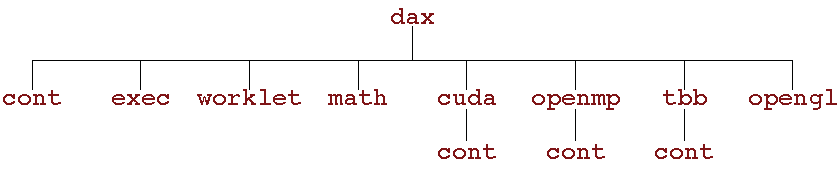
\includegraphics{images/PackageHierarchy}
  \caption{Dax package hierarchy.}
  \label{fig:Packages}
\end{figure}

By convention all classes will be defined in a file with the same name as
the class name (with a \textfilename{.h} extension) located in a directory
corresponding to the package name. For example, the \daxcont{ArrayHandle}
class is found in the \daxheader{dax/cont}{ArrayHandle.h} header. There
are, however, exceptions to this rule. Some smaller classes and types are
grouped together for convenience. These exceptions will be noted as
necessary.

Within each namespace there may also
be \textnamespace{internal}\indexnamespaceone{internal}
and \textnamespace{detail}\indexnamespaceone{detail}
sub-namespaces. The \textnamespace{internal} namespaces contain features
that are used internally and may change without
notice. The \textnamespace{detail} namespaces contain features that are
used by a particular class but must be declared outside of that
class. Users should generally ignore classes in these namespaces.

\index{packages|)}


\section{Basic Provisions}
\label{sec:BasicProvisions}

This section describes the core facilities provided by the Dax
toolkit. These include macros, types, and classes that define the
environment in which code is run, the core types of data stored, and
template introspection.

\subsection{Function and Method Exports}
\label{sec:FunctionAndMethodExports}

Any function or method defined by the Dax toolkit must come with an export
modifier that determines in which environments the function may be
run. These export modifiers are C macros that Dax uses to instruct the
compiler for which architectures to compile each method. Most user code
outside of the Dax toolkit need not use these macros with the important
exception of any classes passed to the Dax toolkit. This occurs when
defining new worklets, array containers, and device adapters.

Dax provides three export macros, \daxcontexport, \daxexecexport, and
\daxexeccontexport, which are used to declare functions and methods that
can run in the control environment, export environment, and both
environments, respectively. These macros get defined by including just
about any Dax header file, but including \daxheader{dax}{Types.h} will
ensure they are defined. 

The export macro is place after the template declaration, if there is one,
and before the return type for the function. Here is a simple example of a
function that will square a value. Since most types you would use this
function on have operators in both the control and execution environments,
the function is exported to both places.

\begin{daxexample}{Usage of export macro.}
template<class ValueType>
DAX_EXEC_CONT_EXPORT
ValueType Square(const ValueType &inValue)
{
 return inValue * inValue;
}
\end{daxexample}

The primary function of the export macros is to interject compiler-specific
keywords that specify what architecture to compile code for. For example,
when compiling with CUDA\index{CUDA}, the control exports have
\textcode{\_\_host\_\_} in them and execution exports have
\textcode{\_\_device\_\_} in them.

There is one additional export macro that is not used for functions but
rather used when declaring a constant data object that is used in the
execution environment. This macro is named
\daxmacro{DAX\_EXEC\_CONSTANT\_EXPORT}\index{export!constant}\index{constant~export}
and is used to declare a constant lookup table used when executing a
worklet. Its primary reason for existing is to add a
\textcode{\_\_constant\_\_} keyword when compiling with CUDA. This export
currently has no effect on any other compiler.

\subsection{Core Data Types}
\label{sec:CoreDataTypes}

Except in rare circumstances where precision is not a concern, the Dax
toolkit does not directly use the core C types like \textcode{int},
\textcode{float}, and \textcode{double}. Instead, Dax provides its own core
types, which are declared in \daxheader{dax}{Types.h}.

\subsubsection{Single Number Types}

All floating point values should be declared as type \dax{Scalar}, and all
integer values, generally used for indexing, should be declared as type
\dax{Id}. The chief advantage of using these declared types rather than the
core C types is that the precision can easily be changed. By default, both
types are 32 bits wide. The CMake configuration options
\cmakevar{DAX\_USE\_DOUBLE\_PRECISION} and \cmakevar{DAX\_USE\_64BIT\_IDS}
can be used to change the \dax{Scalar} type and \dax{Id} type,
respectively, to be 64 bits wide. The configuration can be overridden by
defining the C macro \daxmacro{DAX\_USE\_DOUBLE\_PRECISION} or
\daxmacro{DAX\_NO\_DOUBLE\_PRECISION} to force \dax{Scalar} to be either 64
or 32 bits and defining the C macro \daxmacro{DAX\_USE\_64BIT\_IDS} or
\daxmacro{DAX\_NO\_64BIT\_IDS} to force \dax{Id} to be either 64 or 32
bits. These macros must be defined before any Dax header files are included
to take effect. For convenience, you can include either
\daxheader{dax/internal}{ConfigureFor32.h} or
\daxheader{dax/internal}{ConfigureFor64.h} to force both \dax{Scalar} and
\dax{Id} to be 32 or 64 bits. The reason Dax uses macros to determine these
type widths rather than templates is to reduce the number of template
parameters required in the already template-heavy Dax classes and
functions.

\subsubsection{Vector Types}

Visualization algorithms also often require operations on short
vectors. Arrays indexed in up to three dimensions are common. Data is often
defined in 2-space and 3-space, and transformations are typically done in
homogeneous coordinates of length 4. To simplify these types of operations,
Dax provides several vector data types.

The types \dax{Id2} and \dax{Id3} are couple and triple values of type
\dax{Id}. The types \dax{Vector2}, \dax{Vector3}, and \dax{Vector4} are
couple, triple, and quadruple values of type \dax{Scalar}. The elements of
these vectors are accessed with the bracket operator, so they syntactically
appear like short arrays. They additionally have a constant named
\textidentifier{NUM\_COMPONENTS}\index{NUM\_COMPONENTS} to specify how many
components are in the tuple.

The default constructor of these vector types leaves the values
uninitialized. All vectors have a constructor with one arguments that is
used to initialize all components. All these vectors also have a
constructor that allows you to set the individual components. Likewise,
there are a set of \dax{make\_Id*} and \dax{make\_Vector*} functions that
build initialized vector types.

\begin{daxexample}{Creating vector types.}
dax::Vector3 A(1);                      // A is {1, 1, 1}
A[1] = 2;                               // A is now {1, 2, 1}
dax::Vector3 B(1, 2, 3);                // B is {1, 2, 3}
dax::Vector3 C = make_Vector3(3, 4, 5); // C is {3, 4, 5}
\end{daxexample}

The vector types all support component-wise arithmetic using the operators
for plus (\textcode{+}), minus (\textcode{-}), multiply (\textcode{*}), and
divide (\textcode{/}). They also support scalar to vector multiplication
with the multiply operator. The comparison operators equal (\textcode{==})
is true if every pair of corresponding components are true and not equal
(\textcode{!=}) is true otherwise.  A special \dax{dot} function is
overloaded to provide a dot product for every type of vector.

\begin{daxexample}{Vector operations.}
dax::Vector3 A(1, 2, 3);
dax::Vector3 B(4, 5, 6.5);
dax::Vector3 C = A + B;                     // C is {5, 7, 9.5}
dax::Vector3 D = 2 * C;                     // D is {10, 14, 19}
dax::Scalar s = dax::dot(A, B);             // s is 33.5
bool b1 = (A == B);                         // b1 is false
bool b2 = (A == dax::make_Vector3(1, 2, 3); // b2 is true
\end{daxexample}

\subsubsection{Tuple}

The Dax toolkit provides the templated class \dax{Tuple}\tparams{T,Size},
which is essentially a fixed length array of a given type. \dax{Tuple}
objects behave just like the vector types previously described but with any
type and length that you specify.

\begin{daxexample}{The tuple class.}
dax::Tuple<dax::Scalar, 5> A(2);  // A is {2, 2, 2, 2, 2}
for (int index = 1; index < NUM_COMPONENTS; index++)
  {
  A[index] = A[index-1] * 1.5;
  }
// A is now {2, 3, 4.5, 6.75, 10.125}
\end{daxexample}

The same operators that work on the vector types work on \dax{Tuple} with
the caveat that the operator must work on the component type of the
tuple. For example, the multiply operator will work fine on objects of type
\dax{Tuple}\tparams{char,3}, but the multiply operator will not work on objects
of type \dax{Tuple}\tparams{std::string,3} because you cannot multiply
objects of type \textcode{std::string}.

A \dax{Tuple} of the appropriate type can be used interchangeably with a
matching vector type. In fact, a vector type is really just a typedef over
a \dax{Tuple}. This is convenient for a number of things including writing
generic functions that work over all types.

\begin{daxexample}{Interchangeability of tuples and vector types.}
template<typename T, int Size>
DAX_EXEC_CONT_EXPORT
T SumComponents(const dax::Tuple<T,Size> &tuple)
{
  T result = tuple[0];
  for (int index = 1; index < Size; index++)
    {
    result += tuple[index];
    }
  return result;
}

void Foo()
{
  dax::Id a = SumComponents(dax::make_Id3(1, 2, 3));                    // a is 6
  dax::Scalar b = SumComponents(dax::make_Vector4(1.5, 2.5, 3.5, 4.5)); // b is 12
}
\end{daxexample}

In addition to generalizing vector operations and making arbitrarily long
vectors, \dax{Tuple} is useful for creating any sequence of homogeneous
objects. Here is a simple example of using \dax{Tuple} to hold the state of
a polygon.

\begin{daxexample}{Usage of a tuple.}
dax::Tuple<dax::Vector2,3> equilateralTriange(dax::make_Vector2(0.0, 0.0),
                                              dax::make_Vector2(1.0, 0.0),
                                              dax::make_Vector2(0.5, 0.866));
\end{daxexample}

\subsubsection{Extents}

\dax{Extent3} is a simple structure that holds the extent information for
structured data (data defined on a regular grid). It contains to \dax{Id3}
fields named \textcode{Min} and \textcode{Max} that define the minimum and
maximum. \dax{Extent3} and several associated helper functions are defined
in the \daxheader{dax}{Extent.h} header.

\begin{daxexample}{Creating and using an \textidentifier{Extent3}.}
#include <dax/Extent.h>
#include <dax/Types.h>

void ExtentExample()
{
  // Make an extent that defines a grid that has 5x5x3 points and "centered"
  // at index (0,0,0).
  dax::Extent3 extent(dax::make_Id3(-2,-2,-1), dax::make_Id3(2,2,1));

  dax::Id3 minIndices = extent.Min; // Is (-2,-2,-1)
  dax::Id3 maxIndices = extent.Max; // Is (2,2,1)

  dax::Id3 pointDimensions = extentDimensions(extent); // Returns (5,5,3)
  dax::Id3 cellDimensions = extentCellDimensions(extent); // Returns (4,4,2)

  dax::Id3 pointIndexA = flatIndexToIndex3(31, extent); // Returns (-1,-1,0)
  dax::Id3 cellIndexA = flatIndexToIndex3Cell(31, extent); // Returns (1,1,0)

  dax::Id pointIndexB = index3ToFlatIndex(dax::make_Id3(2,-1,0), extent); // Returns 34
  dax::Id pointIndexB = index3ToFlatIndexCell(dax::make_Id(2,-1,0), extent); // Returns 24
}
\end{daxexample}

\subsubsection{Pair}

The Dax toolkit defines a \dax{Pair}\tparams{T1,T2} templated object that
behaves just like \textcode{std:\colonhyp{}pair} from the standard template
library. The difference is that \dax{Pair} will work in both the execution
and control environment, whereas the STL \textcode{std::pair} does not
always work in the execution environment.

The Dax version of \dax{Pair} supports the same types, fields, and
operations as the STL version. Dax also provides a \dax{make\_Pair}
function for convenience.

\subsection{Traits}
\label{sec:Traits}

\index{traits|(}

When using templated types, it is often necessary to get information about
the type or specialize code based on general properties of the type. The
Dax toolkit uses traits classes to publish and retrieve information about
types. A traits class is simply a templated structure that provides
typedefs for tag\index{tag} structures, empty types used for
identification. The traits classes might also contain constant numbers and
helpful static functions. See Mayers\scite{Mayers2009} for a description of
traits classes and their uses.

\subsubsection{Type Traits}

The \dax{TypeTraits}\tparams{T} templated class provides basic information
about a core type. These type traits are available for all the basic C++
types as well as the core Dax types described in
Section~\ref{sec:CoreDataTypes}. \dax{TypeTraits} contains the following
elements.

\begin{description}
\item[\textidentifier{NumericTag}] \index{NumericTag} This type is set to
  either \dax{TypeTraitsRealTag} or \dax{TypeTraitsIntegerTag} to signal
  that the type represents either floating point numbers or integers.
\item[\textidentifier{DimensionalityTag}] \index{DimensionalityTag} This
  type is set to either \dax{TypeTraitsScalarTag} or
  \dax{TypeTraitsVectorTag} to signal that the type represents either a
  single scalar value or a tuple of values.
\end{description}

The definition of \dax{TypeTraits} for \dax{Scalar} could like something
like this.
\begin{daxexample}{Definition of \protect \dax{TypeTraits}\tparams{\protect \dax{Scalar}}.}
namespace dax {

template<>
struct TypeTraits<dax::Scalar>
{
  typedef TypeTraitsRealTag NumericTag;
  typedef TypeTraitsScalarTag DimensionalityTag;
};

}
\end{daxexample}

Here is a simple example of using \dax{TypeTraits} to implement a generic
function that behaves like the modulus operator (\textcode{\%}) for all
types including floating points and vectors.

\begin{daxexample}[ex:TypeTraits]{Using \textidentifier{TypeTraits} for a generic modulus.}
#include <dax/TypeTraits.h>

template<typename T>
T Modulus(const T &numerator, const T &denominator);

namespace detail {

template<typename T>
T ModulusImpl(const T &numerator,
              const T &denominator,
              dax::TypeTraitsIntegerTag,
              dax::TypeTraitsScalarTag)
{
  return numerator % denominator;
}

template<typename T>
T ModulusImpl(const T &numerator,
              const T &denominator,
              dax::TypeTraitsRealTag,
              dax::TypeTraitsScalarTag)
{
  T quotient = numerator / denominator;
  return (quotient - dax::math::Floor(quotient))*denominator;
}

template<typename T, typename NumericTag>
T ModulusImpl(const T &numerator,
              const T &denominator,
              NumericTag,
              dax::TypeTraitsVectorTag)
{
  T result;
  for (int componentIndex = 0; componentIndex < T::NUM_COMPONENTS; componentIndex++)
    {
    result[componentIndex] = Modulus(numerator[componentIndex],denominator[componentIndex]);
    }
}

} // namespace detail

template<typename T>
T Modulus(const T &numerator, const T &denominator)
{
  return detail::ModulusImpl(numerator,
                             denominator,
                             typename dax::TypeTraits<T>::NumericTag(),
                             typename dax::TypeTraits<T>::DimensionalityTag());
}
\end{daxexample}

\subsubsection{Vector Traits}

The \dax{VectorTraits}\tparams{T} templated class provides information and
accessors to vector and tuple types. It contains the following elements.

\begin{description}
\item[\textidentifier{ComponentType}] \index{ComponentType} This type is
  set to the type for each component in the vector. For example, a
  \dax{Vector3} has \textidentifier{ComponentType} defined as \dax{Scalar}.
\item[\textidentifier{NUM\_COMPONENTS}] \index{NUM\_COMPONENTS} An integer
  specifying how many components are contained in the vector.
\item[\textidentifier{HasMultipleComponents}] \index{HasMultipleComponents}
  This type is set to either \dax{VectorTraitsTagSingleComponent} if the
  vector length is size 1 or \dax{VectorTraitsTagMultipleComponents}
  otherwise. This tag can be useful for creating specialized functions when
  a vector is really just a scalar.
\item[\textcode{GetComponent}] \index{GetComponent} A static method that
  takes a vector and returns a particular component.
\item[\textcode{SetComponent}] \index{SetComponent} A static method that
  takes a vector and sets are particular component to a given value.
\item[\textcode{ToTuple}] \index{ToTuple} A static method that converts a
  vector of the given type to a \dax{Tuple}.
\end{description}

The definition of \dax{VectorTraits} for \dax{Id3} could like something
like this.
\begin{daxexample}{Definition of \protect \dax{VectorTraits}\tparams{\protect \dax{Id3}}.}
template<>
struct VectorTraits<dax::Id3>
{
  typedef dax::Id ComponentType;
  static const int NUM_COMPONENTS = 3;
  typedef VectorTraitsTagMultipleComponents HasMultipleComponents;

  DAX_EXEC_CONT_EXPORT
  static dax::Id &GetComponent(dax::Id3 &vector, int component) {
    return vector[component];
  }

  DAX_EXEC_CONT_EXPORT
  static void SetComponent(dax::Id3 &vector, int component, dax::Id value) {
    vector[component] = value;
  }

  DAX_EXEC_CONT_EXPORT
  static dax::Tuple<dax::Id,3> ToTuple(const dax::Id3 &vector) {
    return vector;
  }
};
\end{daxexample}

The real power of vector traits is that they simplify creating generic
operations on any type that can look like a vector. This includes
operations on scalar values as if they were vectors of size one. The
following code uses vector traits to simplify the implementation of less
functors\index{less} that define an ordering that can be used for sorting
and other operations.

\begin{daxexample}{Using \textidentifier{VectorTraits} for less functors.}
#include <dax/VectorTraits.h>

// This functor provides a total ordering of vectors. Every compared vector
// will be either less, greater, or equal.
template<typename T>
struct LessTotalOrder
{
  bool operator()(const T &left, const T &right)
  {
    for (int index = 0; index < dax::VectorTraits<T>::NUM_COMPONENTS; index++)
      {
      const T &leftValue = dax::VectorTraits<T>::GetComponent(left, index);
      const T &rightValue = dax::VectorTraits<T>::GetComponent(right, index);
      if (leftValue < rightValue) { return true; }
      if (rightValue < leftValue) { return false; }
      }
    // If we are here, the vectors are equal.
    return false;
  }
};

// This functor provides a partial ordering of vectors. It returns true if and
// only if all components satisfy the less operation. It is possible for
// vectors to be neither less, greater, nor equal, but the transitive closure
// is still valid.
template<typename T>
struct LessTotalOrder
{
  bool operator()(const T &left, const T &right)
  {
    for (int index = 0; index < dax::VectorTraits<T>::NUM_COMPONENTS; index++)
      {
      const T &leftValue = dax::VectorTraits<T>::GetComponent(left, index);
      const T &rightValue = dax::VectorTraits<T>::GetComponent(right, index);
      if (!(leftValue < rightValue)) { return false; }
      }
    // If we are here, all components satisfy less than relation.
    return true;
  }
};
\end{daxexample}

\index{traits|)}

%TODO: Document vector operations


\section{Provided Worklets}
\label{sec:ProvidedWorklets}

The Dax toolkit provides several common visualization algorithms
encapsulated in worklets\index{worklet} that can be executed in parallel on
your data. This section describes each of the worklets provided. All
worklets provided by Dax are in the \daxworklet{} namespace and defined in
header files in the \textfilename{dax/worklet} directory.

Much of the support structures for defining data and executing jobs, which
you will see in examples, is defined in the Dax control
environment\index{control~environment}. These features are documented in
Section~\ref{sec:ControlEnvironment}. The Dax toolkit also provides
facilities to make it easy to define your own worklet. Descriptions of
these features are in Section~\ref{sec:ExecutionEnvironment}.

\subsection{Cell Average}
\label{sec:worklet:CellAverage}

The \daxworklet{CellAverage} worklet takes a topology and a field and
averages the value of the field in each point. For each cell, it find the
field value on each point of the cell and takes the average of
those. \daxworklet{CellAverage} is a cheap but inaccurate way to integrate
the value of a field in each cell. A similar worklet named point data to
cell data does a similar operation except that it interpolates the field
value to the parametric center of the cell
(Section~\ref{sec:worklet:PointDataToCellData}), which may be different
than a simple average.

\begin{daxexample}{Cell average worklet.}
#include <dax/worklet/CellAverage.h>

#include <dax/cont/ArrayHandle.h>
#include <dax/cont/Scheduler.h>

template<typename GridType>
DAX_CONT_EXPORT
void RunCellAverage(const GridType &grid,
                    const dax::cont::ArrayHandle<dax::Scalar> &inPointData,
                    dax::cont::ArrayHandle<dax::Scalar> &outCellData)
{
  dax::cont::Scheduler<> scheduler;
  scheduler.Invoke(dax::worklet::CellAverage(), grid, inPointData, outCellData);
}
\end{daxexample}

\subsection{Cell Data to Point Data}

The cell data to point data worklet finds all cells incident on each point
and then averages the field values of all incident cells to the point.

\fix{TODO: Running this worklet needs to be simplified. The scheduler needs
  to be cleaned up to remove the helper classes. Also, there should
  probably be a specialized worklet type for doing cell to point
  operations.}

Running the cell data to point data worklet is a two step process. In the
first step, \daxworklet{CellDataToPointDataGenerateKeys} extracts point
indices for each cell and attaches field values to them. In the second
step, \daxworklet{CellDataToPointDataReduceKeys} collects field values on a
point and averages them.

\begin{daxexample}{Cell data to point data worklet.}
#include <dax/worklet/CellDataToPointData.h>

#include <dax/cont/ArrayHandle.h>
#include <dax/cont/ArrayHandleConstant.h>
#include <dax/cont/GenerateKeysValues.h>
#include <dax/cont/ReduceKeysValues.h>
#include <dax/cont/Scheduler.h>

#include <dax/CellTraits.h>

template<typename GridType, typename FieldType>
DAX_CONT_EXPORT
void RunCellDataToPointData(const GridType &grid,
                            const dax::cont::ArrayHandle<FieldType> &inPointData,
                            dax::cont::ArrayHandle<FieldType> &outCellData)
{
  dax::cont::ArrayHandleConstant<dax::Id> keyGenCounts =
      dax::cont::make_ArrayHandleConstant<dax::Id>(
            dax::CellTraits<CellTag>::NUM_VERTICES, grid.GetNumberOfCells());  

  dax::cont::Scheduler<> scheduler;

  dax::cont::GenerateKeysValues<
      dax::worklet::CellDataToPointDataGenerateKeys,
      dax::cont::ArrayHandleConstant<dax::Id> > generateKeys(keyGenCounts);

  dax::cont::ArrayHandle<dax::Id> keyArray;
  dax::cont::ArrayHandle<FieldType> valueArray;

  scheduler.Invoke(generateKeys, grid, inPointData, keyArray, valueArray);

  dax::cont::ReduceKeysValues<
    dax::worklet::CellDataToPointDataReduceKeys,
    dax::cont::ArrayHandle<dax::Id> > reduceKeys(keyArray);

  scheduler.Invoke(reduceKeys, valueArray, outCellData);
}
\end{daxexample}

\subsection{Cell Gradient}

The \daxworklet{CellGradient} worklet computes the gradient of a point
field at the parametric center of each cell.

\begin{daxexample}{Cell gradient worklet.}
#include <dax/worklet/CellGradient.h>

#include <dax/cont/ArrayHandle.h>
#include <dax/cont/Scheduler.h>

template<typename GridType>
DAX_CONT_EXPORT
void RunCellGradient(const GridType &grid,
                     const dax::cont::ArrayHandle<dax::Scalar> &inPointField,
                     dax::cont::ArrayHandle<dax::Vector3> &outCellGradient)
{
  dax::cont::Scheduler<> scheduler;
  scheduler.Invoke(dax::worklet::CellGradient(),
                   grid,
                   grid.GetPointCoordinates(),
                   inPointField,
                   outCellGradient);
}
\end{daxexample}

\subsection{Cosine}

The \daxworklet{Cosine} worklet computes the cosine of a field. The field
can be either a point field or a cell field (or really, just any array).

\begin{daxexample}{Cosine worklet.}
#include <dax/worklet/Cosine.h>

#include <dax/cont/ArrayHandle.h>
#include <dax/cont/Scheduler.h>

template<typename FieldType>
DAX_CONT_EXPORT
void RunCosine(const dax::cont::ArrayHandle<FieldType> &inField,
               dax::cont::ArrayHandle<FieldType> &outField)
{
  dax::cont::Scheduler<> scheduler;
  scheduler.Invoke(dax::worklet::Cosine(), inField, outField);
}
\end{daxexample}

\subsection{Elevation}

The \daxworklet{Elevation} worklet find the elevation of points in
$\mathrm{R}^3$ in relation to a base plane. The orientation of the
elevation is determined by a low point location and a high point
location. Values lower than the low point and higher than the high point
are clamped to the minimum and maximum values. The range of valid values
can also be specified.

The elevation worklet is design to be run on the point coordinates of a
grid, but in fact could be run on any field or array.

The following example demonstrates finding the elevation of points in a
data set oriented along the x axis. Points between $x=-1$ and $x=1$ are
considered. The scale and bias is set to give the distance from the origin
along the x-axis in the positive direction.

\begin{daxexample}[ex:Elevation]{Elevation worklet.}
#include <dax/worklet/Elevation.h>

#include <dax/cont/ArrayHandle.h>
#include <dax/cont/Scheduler.h>

template<typename GridType>
DAX_CONT_EXPORT
void Elevation(const GridType &grid,
               dax::cont::ArrayHandle<dax::Scalar> &outPointElevation)
{
  dax::worklet::Elevation elevation(dax::make_Vector3(-1.0, 0.0, 0.0),
                                    dax::make_Vector3(1.0, 0.0, 0.0),
                                    dax::make_Vector2(-1.0, 1.0));

  dax::cont::Scheduler<> scheduler;
  scheduler.Invoke(elevation, grid.GetPointCoordinates(), outPointElevation);
}
\end{daxexample}

\subsection{Magnitude}

The \daxworklet{Magnitude} worklet computes the magnitude of a field of
vectors. The field can be either a point field or a cell field (or really,
just any array).

\begin{daxexample}{Magnitude worklet.}
#include <dax/worklet/Magnitude.h>

#include <dax/cont/ArrayHandle.h>
#include <dax/cont/Scheduler.h>

DAX_CONT_EXPORT
void RunMagnitude(const dax::cont::ArrayHandle<dax::Vector3> &inField,
                  dax::cont::ArrayHandle<dax::Scalar> &outField)
{
  dax::cont::Scheduler<> scheduler;
  scheduler.Invoke(dax::worklet::Magnitude(), inField, outField);
}
\end{daxexample}

\subsection{Marching Cubes}

The Marching Cubes worklet takes a volume and extracts the contour surface
where a field value is equal to a given value.

\fix{TODO: Running this worklet needs to be simplified. The scheduler needs
  to be cleaned up to remove the helper classes.}

Running the Marching Cubes worklet is a two step process. In the first
step, \daxworklet{MarchingCubesClassify} identifies how many polygons are
going to be generated for every input cell. In the second step,
\daxworklet{MarchingCubesGenerate} creates the triangles that make up the
surface.

\begin{daxexample}{Marching Cubes worklet.}
#include <dax/worklet/MarchingCubes.h>

#include <dax/cont/ArrayHandle.h>
#include <dax/cont/GenerateInterpolatedCells.h>
#include <dax/cont/Scheduler.h>
#include <dax/cont/UnstructuredGrid.h>

template<typename GridType>
DAX_CONT_EXPORT
void RunMarchingCubes(const GridType &inGrid,
                      const dax::cont::ArrayHandle<FieldType> &inPointData,
                      dax::Scalar isovalue,
                      dax::cont::UnstructuredGrid<dax::CellTagTriangle> &outGrid)
{
  dax::cont::Scheduler<> scheduler;

  dax::cont::ArrayHandle<dax::Id> classification;
  scheduler.Invoke(dax::worklet::MarchingCubesClassify(isovalue),
                   inGrid,
                   inPointData,
                   classification);

  dax::cont::GenerateInterpolatedCells<
    dax::worklet::MarchingCubesGenerate, dax::cont::ArrayHandle<dax::Id> >
        generate(dax::worklet::MarchingCubesGenerate(isovalue), classification);
  scheduler.Invoke(generate, inGrid, outGrid, inPointData);
}
\end{daxexample}

\subsection{Point Data to Cell Data}
\label{sec:worklet:PointDataToCellData}

The \daxworklet{PointDataToCellData} worklet takes a topology and a field
and averages the value of the field in each point. For each cell, it
interpolates a point field to the center of the cell. A similar worklet
named cell average does a similar operation except that simply averages the
field values (Section~\ref{sec:worklet:CellAverage}), which may be
different than the interpolation.

The following example uses \daxworklet{PointDataToCellData} to find the
coordinates of each cell center.

\begin{daxexample}{Point data to cell data worklet.}
#include <dax/worklet/PointDataToCellData.h>

#include <dax/cont/ArrayHandle.h>
#include <dax/cont/Scheduler.h>

template<typename GridType>
DAX_CONT_EXPORT
void RunPointDataToCellData(const GridType &grid,
                            dax::cont::ArrayHandle<dax::Scalar> &outCellCenters)
{
  dax::cont::Scheduler<> scheduler;
  scheduler.Invoke(dax::worklet::PointDataToCellData(),
                   grid,
                   grid.GetPointCoordinates(),
                   Centers);
}
\end{daxexample}

\subsection{Sine}

The \daxworklet{Sine} worklet computes the sine of a field. The field
can be either a point field or a cell field (or really, just any array).

\begin{daxexample}{Sine worklet.}
#include <dax/worklet/Sine.h>

#include <dax/cont/ArrayHandle.h>
#include <dax/cont/Scheduler.h>

template<typename FieldType>
DAX_CONT_EXPORT
void RunSine(const dax::cont::ArrayHandle<FieldType> &inField,
             dax::cont::ArrayHandle<FieldType> &outField)
{
  dax::cont::Scheduler<> scheduler;
  scheduler.Invoke(dax::worklet::Sine(), inField, outField);
}
\end{daxexample}

\subsection{Slice}

The slice worklet takes a volume and intersects it with a plane.

\fix{TODO: Running this worklet needs to be simplified. The scheduler needs
  to be cleaned up to remove the helper classes.}

Running the slice worklet is a two step process. In the first step,
\daxworklet{SliceClassify} identifies how many polygons are going to be
generated for every input cell. In the second step,
\daxworklet{SliceGenerate} creates the triangles that make up the surface
that is the intersection of the volume and the plane.

\begin{daxexample}{Slice worklet.}
#include <dax/worklet/Slice.h>

#include <dax/cont/ArrayHandle.h>
#include <dax/cont/GenerateInterpolatedCells.h>
#include <dax/cont/Scheduler.h>
#include <dax/cont/UnstructuredGrid.h>

template<typename GridType>
DAX_CONT_EXPORT
void RunSlice(const GridType &inGrid,
              const dax::cont::ArrayHandle<FieldType> &inPointData,
              dax::Scalar isovalue,
              dax::cont::UnstructuredGrid<dax::CellTagTriangle> &outGrid)
{
  dax::cont::Scheduler<> scheduler;

  dax::cont::ArrayHandle<dax::Id> classification;
  scheduler.Invoke(dax::worklet::SliceClassify(isovalue),
                   inGrid,
                   inPointData,
                   classification);

  dax::cont::GenerateInterpolatedCells<
    dax::worklet::SliceGenerate, dax::cont::ArrayHandle<dax::Id> >
        generate(dax::worklet::SliceGenerate(isovalue), classification);
  scheduler.Invoke(generate, inGrid, outGrid, inPointData);
}
\end{daxexample}

\subsection{Square}

The \daxworklet{Square} worklet computes the square of all the values in a
field. (It finds a component-wise square in the case of vector types.) The
field can be either a point field or a cell field (or really, just any
array).

\begin{daxexample}{Square worklet.}
#include <dax/worklet/Square.h>

#include <dax/cont/ArrayHandle.h>
#include <dax/cont/Scheduler.h>

template<typename FieldType>
DAX_CONT_EXPORT
void RunSquare(const dax::cont::ArrayHandle<FieldType> &inField,
               dax::cont::ArrayHandle<FieldType> &outField)
{
  dax::cont::Scheduler<> scheduler;
  scheduler.Invoke(dax::worklet::Square(), inField, outField);
}
\end{daxexample}

\subsection{Tetrahedralize}

The \daxworklet{Tetrahedralize} takes a data set and divides each cell into
a group of simplices (tetrahedra) that comprise the volume.

\fix{TODO: Running this worklet needs to be simplified. The scheduler needs
  to be cleaned up to remove the helper classes. There is also some
  hinkiness involved with specifying the count (classification) array.}

\begin{daxexample}{Tetrahedralize worklet.}
#include <dax/worklet/Tetrahedralize.h>

#include <dax/cont/ArrayHandleConstant.h>
#include <dax/cont/GenerateTopology.h>
#include <dax/cont/Scheduler.h>
#include <dax/cont/UnstructuredGrid.h>

template<typename GridType>
DAX_CONT_EXPORT
void RunTetrahedralize(const GridType &inGrid,
                       dax::cont::UnstructuredGrid<dax::CellTagTetrahedron> &outGrid)
{
  typedef dax::cont::ArrayHandleConstant<dax::Id> ClassificationType;
  ClassificationType classification(5, inGrid.GetNumberOfCells());

  dax::cont::GenerateTopology<dax::worklet::Tetrahedralize,ClassificationType>
      generate(classification);
  generate.SetRemoveDuplicatePoints(false);

  dax::cont::Scheduler<> scheduler;
  scheduler.Invoke(generate, inGrid, outGrid);
}
\end{daxexample}

\subsection{Threshold}

The threshold worklet takes a grid and extracts all cells with field values
within a range specified by a minimum and maximum value.

\fix{TODO: Running this worklet needs to be simplified. The scheduler needs
  to be cleaned up to remove the helper classes.}

Running the threshold worklet is a two step process. In the first step,
\daxworklet{ThresholdClassify} identifies how many cells are going to be
generated for every input cell (0 or 1). In the second step,
\daxworklet{ThresholdTopology} creates a new grid with the passed cells.

\begin{daxexample}{Threshold worklet.}
#include <dax/worklet/Threshold.h>

#include <dax/cont/ArrayHandle.h>
#include <dax/cont/GenerateTopology.h>
#include <dax/cont/Scheduler.h>
#include <dax/cont/UnstructuredGrid.h>

template<typename CellType, typename FieldType>
DAX_CONT_EXPORT
void RunThreshold(const dax::cont::UnstructuredGrid<CellType> &inGrid,
                  const dax::cont::ArrayHandle<FieldType> &inPointField,
                  FieldType thresholdMin,
                  FieldType thresholdMax,
                  dax::cont::UnstructuredGrid<CellType> &outGrid,
                  dax::cont::ArrayHandle<FieldType> &outPointField)
{
  dax::cont::Scheduler<> scheduler;
  
  typedef dax::cont::ArrayHandle<dax::Id> ClassificationType;
  ClassificationType classification;

  scheduler.Invoke(dax::worklet::ThresholdClassify<FieldType>(thresholdMin, thresholdMax),
                   inGrid,
                   inPointField,
                   classification);

  dax::cont::GenerateTopology<dax::worklet::ThresholdTopology,ClassificationType>
      generate(classification);

  scheduler.Invoke(generate, inGrid, outGrid);

  generate.CompactPointField(inPointField, outPointField);
}
\end{daxexample}


\section{Control Environment}
\label{sec:ControlEnvironment}

\index{control~environment|(}

The control environment is where code interfaces with applications and
I/O devices. The associated API is designed for users that want to use the
Dax toolkit to analyze their data using provided or supplied worklets. Code
for the control environment is designed to run on a single thread (or one
single thread per process in an MPI job).

Most users of the Dax toolkit will have some interaction with the Dax
toolkit, for you cannot define data structures or execute any algorithms
without it.

\subsection{Device Adapter Tag}
\label{sec:DeviceAdapterTag}

\index{device~adapter|(}

The Dax toolkit uses a feature called a device adapter to define what type
of device will be used to run algorithms. The device adapter encapsulates
the device-specific code required to port to various devices. More
information on the function of the device adapter are given in
Section~\ref{sec:DeviceIndependence}.

The device adapter is identified by a \keyterm{device adapter tag}.
\index{device~adapter~tag} This tag, which is simply an empty struct type,
is used as the template parameter for several classes in the Dax control
environment and causes these classes to direct their work to a particular
device.

There are two ways to select a device adapter. The first is to make a
global selection of a default device adapter. The second is to specify a
specific device adapter as a template parameter.

\subsubsection{Default Device Adapter}

A default device adapter tag is specified in
\daxheader{dax/cont}{DeviceAdapter.h} (although it can also by specified in
many other Dax headers via header dependencies). If no other information is
given, Dax attempts to choose a default device adapter that is a best fit
for the system it is compiled on. Dax currently select the default device
adapter with the following sequence of conditions.

\begin{itemize}
\item \index{CUDA} If the source code is being compiled by CUDA, the CUDA
  device is used.
\item \index{OpenMP} If the CUDA compiler is not being used and the current
  compiler supports OpenMP, then the OpenMP device is used.
\item \index{Intel Threading Building Blocks} \index{TBB} If the compiler
  supports neither CUDA nor OpenMP and the Dax Toolkit was configured to
  use Intel Threading Building Blocks, then that device is used.
\item \index{serial} If no parallel device adapters are found, then the Dax
  Toolkit falls back to a serial device.
\end{itemize}

You can also set the default device adapter specifically by setting the
\daxmacro{DAX\_DEVICE\_ADAPTER} macro. This macro must be set \emph{before}
including any Dax header files. You can set \daxmacro{DAX\_DEVICE\_ADAPTER}
to any one of the following.

\begin{description}
\item[\daxmacro{DAX\_DEVICE\_ADAPTER\_SERIAL}] Performs all computation on
  the same single thread as the control environment. This device is useful
  for debugging. This device is always available.
\item[\daxmacro{DAX\_DEVICE\_ADAPTER\_CUDA}] Uses a CUDA capable GPU
  device. For this device to work, Dax must be configured to use CUDA and
  the code must be compiled by the CUDA \textfilename{nvcc} compiler.
\item[\daxmacro{DAX\_DEVICE\_ADAPTER\_OPENMP}] Uses OpenMP compiler
  extensions to run algorithms on multiple threads. For this device to
  work, Dax must be configured to use OpenMP and the code must be compiled
  with a compiler that supports OpenMP pragmas.
\item[\daxmacro{DAX\_DEVICE\_ADAPTER\_TBB}] Uses the Intel Threading
  Building Blocks library to run algorithms on multiple threads. For this
  device to work, Dax must be configured to use TBB and the executable must
  be linked to the TBB library.
\end{description}

These macros provide a useful mechanism for quickly reconfiguring code to
run on different devices. The following example shows a typical block of
code at the top of a source file that could be used for quick
reconfigurations.

\begin{daxexample}{Macros to port Dax code among different devices}
// Uncomment one (and only one) of the following to reconfigure the Dax
// code to use a particular device. Comment them all to automatically pick a
// device.
//#define DAX_DEVICE_ADAPTER DAX_DEVICE_ADAPTER_SERIAL
#define DAX_DEVICE_ADAPTER DAX_DEVICE_ADAPTER_CUDA
//#define DAX_DEVICE_ADAPTER DAX_DEVICE_ADAPTER_OPENMP
//#define DAX_DEVICE_ADAPTER DAX_DEVICE_ADAPTER_TBB

#include <dax/cont/DeviceAdapter.h>
\end{daxexample}

The default device adapter can always be overridden by specifying a device
adapter tag, as described in the next section. There is actually one more
internal default device adapter named
\daxmacro{DAX\_DEVICE\_ADAPTER\_ERROR} that will cause a compile error if
any component attempts to use the default device adapter. This feature is
most often used in testing code to check when device adapters should be
specified.

\subsubsection{Specifying Device Adapter Tags}

In addition to setting a global default device adapter, it is possible to
explicitly set which device adapter to use in any feature provided by
Dax. This is done by providing a device adapter tag as a template argument
to Dax templated objects. The following device adapter tags are available
in Dax.

\begin{description}
\item[\daxcont{DeviceAdapterTagSerial}] \index{serial} Performs all
  computation on the same single thread as the control environment. This
  device is useful for debugging. This device is always available. This tag
  is defined in \daxheader{dax/cont}{DeviceAdapterSerial.h}.
\item[\daxcudacont{DeviceAdapterTagCuda}] \index{CUDA} Uses a CUDA capable
  GPU device. For this device to work, Dax must be configured to use CUDA
  and the code must be compiled by the CUDA \textfilename{nvcc}
  compiler. This tag is defined in
  \daxheader{dax/cuda/cont}{DeviceAdapterCuda.h}.
\item[\daxopenmpcont{DeviceAdapterTagOpenMP}] \index{OpenMP} Uses OpenMP
  compiler extensions to run algorithms on multiple threads. For this
  device to work, Dax must be configured to use OpenMP and the code must be
  compiled with a compiler that supports OpenMP pragmas. This tag is
  defined in \daxheader{dax/openmp/cont}{DeviceAdapterOpenMP.h}.
\item[\daxtbbcont{DeviceAdapterTagTBB}]
  \index{Intel Threading Building Blocks} \index{TBB} Uses the Intel
  Threading Building Blocks library to run algorithms on multiple
  threads. For this device to work, Dax must be configured to use TBB and
  the executable must be linked to the TBB library. This tag is defined in
  \daxheader{dax/tbb/cont}{DeviceAdapterTBB.h}.
\end{description}

The following example schedules the elevation worklet much like shown in
Example~\ref{ex:Elevation} on page~\pageref{ex:Elevation} but also
specifies using the Intel Threading Building blocks device adapter.
\index{Intel Threading Building Blocks} \index{TBB}
In particular, consider the template parameter of the \daxcont{Scheduler}
class.
\begin{daxexample}{Calling the Elevation worklet with a specific device adapter.}
dax::worklet::Elevation elevation(dax::make_Vector3(-1.0, 0.0, 0.0),
                                  dax::make_Vector3(1.0, 0.0, 0.0),
                                  dax::make_Vector2(-1.0, 1.0));

dax::cont::Scheduler<dax::tbb::cont::DeviceAdapterTagTBB> scheduler;
scheduler.Invoke(elevation, grid.GetPointCoordinates(), outPointElevation);
\end{daxexample}

When structuring your code to always specify a particular device adapter,
consider setting the default device adapter (with the
\daxmacro{DAX\_DEVICE\_ADAPTER} macro) to
\daxmacro{DAX\_DEVICE\_ADAPTER\_ERROR}. This will cause the compiler to
produce an error if any object is instantiated with the default device
adapter, which checks to make sure the code properly specifies every device
adapter parameter.

The Dax toolkit also defines a macro named
\daxmacro{DAX\_DEFAULT\_DEVICE\_ADAPTER\_TAG} that can be used in place of
an explicit device adapter tag to use the default tag. This macro is used
to create new templates that have template parameters for device adapters
that can use the default. The following example has a (rather artificial)
declaration of a helper class for executing the elevation worklet.
\begin{daxexample}{Declaring a template with a default device adapter.}
template<typename DeviceAdapter = DAX_DEFAULT_DEVICE_ADAPTER_TAG>
class MyElevationScheduler
{
public:
  void DoSchedule()
  {
    dax::cont::Scheduler<DeviceAdapter> scheduler;
    scheduler.Invoke(dax::Worklet::Elevation(),
                     this->Grid.GetPointCoordinates(),
                     this->OutPointElevation);
\end{daxexample}

\index{device~adapter|)}

\subsection{Array Handle}
\label{sec:ArrayHandle}

\index{array~handle|(}

An \keyterm{array handle}, implemented with the \daxcont{ArrayHandle}
class, manages an array of data that can be accessed or manipulated by Dax
algorithms. It is typical to construct an array handle in the control
environment to pass data to an algorithm running in the execution
environment. It is also typical for an algorithm running in the execution
environment to allocate and populate an array handle, which can then be
read back in the control environment. It is also possible for an array
handle to manage data created by one Dax algorithm and passed to another,
remaining in the execution environment the whole time and never copied to
the control environment.

The array handle may have up to two copies of the array, one for the
control environment and one for the execution environment. However,
depending on the device and how the array is being used, the array handle
will only have one copy when possible. Copies between the environments are
implicit and lazy. They are copied only when an operation needs data in an
environment where the data is not.

\daxcont{ArrayHandle} behaves like a shared smart pointer in that when the
C++ object is copied, each copy holds a reference to the same array. These
copies are reference counted so that when all copies of the
\daxcont{ArrayHandle} are destroyed, any allocated memory is released.

\subsubsection{Creating Array Handles}

\daxcont{ArrayHandle} is a templated class with three template
parameters. The first template parameter is the only one required and
specifies the base type of the entries in the array. The second template
parameter specifies the container used when storing data in the control
environment. Containers are discussed later in this section, and for now we
will use the default value. The third template parameter is a device
adapter tag that specifies what device is used in the execution
environment. Device adapter tags are described in
Section~\ref{sec:DeviceAdapterTag}. Most of the examples here will use the
default device adapter.

\begin{daxexample}{Declaration of the \protect\daxcont{ArrayHandle} templated class.}
template<
    typename T,
    typename ArrayContainerControlTag = DAX_DEFAULT_ARRAY_CONTAINER_CONTROL_TAG,
    typename DeviceAdapterTag = DAX_DEFAULT_DEVICE_ADAPTER_TAG>
class ArrayHandle;
\end{daxexample}

There are multiple ways to create and populate an array handle. The default
\daxcont{ArrayHandle} constructor will create an empty array with nothing
allocated in either the control or execution environment. This is
convenient for creating arrays used as the output for algorithms.

\begin{daxexample}{Creating an \textidentifier{ArrayHandle} for output data.}
dax::cont::ArrayHandle<dax::Scalar> outputArray;
\end{daxexample}

Constructing an \daxcont{ArrayHandle} that points to a provided C array or
\textcode{std::vector} is straightforward with the
\daxcont{make\_ArrayHandle} functions. These functions will make an array
handle that points to the array data that you provide.

\begin{daxexample}{Creating an \textidentifier{ArrayHandle} that points to a provided C array.}
dax::Scalar dataBuffer[50];
// Populate dataBuffer with meaningful data. Perhaps read data from a file.

dax::cont::ArrayHandle<dax::Scalar> inputArray = dax::cont::make_ArrayHandle(dataBuffer,50);
\end{daxexample}

\begin{daxexample}[ex:ArrayHandleFromVector]{Creating an \textidentifier{ArrayHandle} that points to a provided \textcode{std::vector}.}
std::vector<dax::Scalar> dataBuffer;
// Populate dataBuffer with meaningful data. Perhaps read data from a file.

dax::cont::ArrayHandle<dax::Scalar> inputArray = dax::cont::make_ArrayHandle(dataBuffer);
\end{daxexample}

\emph{Be aware} that \daxcont{make\_ArrayHandle} makes a shallow pointer
copy. This means that if you change or delete the data provided, the
internal state of \daxcont{ArrayHandle} becomes invalid and undefined
behavior can ensue. The most common manifestation of this error happens
when a \textcode{std::vector} goes out of scope. This subtle interaction
will cause the \daxcont{ArrayHandle} to point to an unallocated portion of
the memory heap. For example, if the code in
Example~\ref{ex:ArrayHandleFromVector} where to be placed within a callable
function or method, it could cause the \daxcont{ArrayHandle} to become
invalid.

\begin{daxexample}{Invalidating an \textidentifier{ArrayHandle} by letting the source \textcode{std::vector} leave scope.}
DAX_CONT_EXPORT
dax::cont::ArrayHandle<dax::Scalar> BadDataLoad()
{
  std::vector<dax::Scalar> dataBuffer;
  // Populate dataBuffer with meaningful data. Perhaps read data from a file.

  dax::cont::ArrayHandle<dax::Scalar> inputArray = dax::cont::make_ArrayHandle(dataBuffer);

  return inputArray;
  // THIS IS WRONG! At this point dataBuffer goes out of scope and deletes its memory.
  // However, inputArray has a pointer to that memory, which becomes an invalid pointer
  // in the returned object. Bad things will happen when the ArrayHandle is used.
}

DAX_CONT_EXPORT
dax::cont::ArrayHandle<dax::Scalar> SafeDataLoad()
{
  std::vector<dax::Scalar> dataBuffer;
  // Populate dataBuffer with meaningful data. Perhaps read data from a file.

  dax::cont::ArrayHandle<dax::Scalar> tmpArray = dax::cont::make_ArrayHandle(dataBuffer);

  // This copies the data from one ArrayHandle to another (in the execution environment).
  // Although it is an extraneous copy, it is usually pretty fast on a parallel device.
  // Another option is to make sure that the buffer in the std::vector never goes out
  // of scope before all the ArrayHandle references, but this extra step allows the
  // ArrayHandle to manage its own memory and ensure everything is valid.
  dax::cont::ArrayHandle<dax::Scalar> inputArray;
  dax::cont::DeviceAdapterAlgorithm<DAX_DEFAULT_DEVICE_ADAPTER_TAG>::Copy(
      tmpArray, inputArray);

  return inputArray;
  // This is safe.
}
\end{daxexample}

\subsubsection{Retrieving Data from an Array Handle}

An array handle does not provide direct access to its underlying data by
design. The most straightforward way to get data from an array handle is to
use the \textcode{CopyInto} method. \textcode{CopyInto} takes an
STL-compatible forward iterator and copies all the data into that
iterator. It is assumed that the iterator can be advanced enough to copy
all data into the target array. The number of entries in the array handle
can be retrieved with the \textcode{GetNumberOfValues} method, and the
target array should be at least that big.

\begin{daxexample}[ex:ArrayHandle::CopyInto]{Retrieving \textidentifier{ArrayHandle} data with \textcode{CopyInto}.}
dax::cont::ArrayHandle<dax::Scalar> outArray;
// Do something that fills outArray

std::vector<dax::Scalar> resultBuffer(outArray.GetNumberOfValues());
outArray.CopyInto(resultBuffer.begin());
\end{daxexample}

There are two other ways data can be retrieved from an array handle. The
first is to request an array portal to the data and the second is to define
a new container that points to a particular data structure. Both of these
methods are discussed in more detail in later sections.

\subsubsection{Array Portals}
\label{sec:ArrayPortals}

\index{array~portal|(}

An array handle defines auxiliary structures called \keyterm{array portals}
that provide direct access into its data. An array portal is a simple
object that is somewhat functionally equivalent to an STL-type iterator, but
with a much simpler interface. Array portals can be read-only (const) or
read-write and they can be accessible from either the control environment
or the execution environment. All these variants have similar interfaces
although some features that are not applicable can be left out.

An array portal object contains each of the following:
\begin{description}
\item[\textcode{ValueType}] A \textcode{typedef} of the type for each item
  in the array.
\item[\textcode{GetNumberOfValues}] A method that returns the number of
  entries in the array.
\item[\textcode{Get}] A method that returns the value at a given index.
\item[\textcode{Set}] A method that changes the value at a given
  index. This method does not need to exist for read-only (const) array
  portals.
\item[\textcode{IteratorType}] A \textcode{typedef} of an STL-compatible
  random-access iterator that can be used for alternative access. This
  method does not need to exist in the execution environment.
\item[\textcode{GetIteratorBegin}] A method that returns an STL-compatible
  iterator of type \textcode{IteratorType} that points to the beginning of
  the array. This method does not need exist in the execution environment.
\item[\textcode{GetIteratorEnd}] A method that returns an STL-compatible
  iterator of type \textcode{IteratorType} that points to the beginning of
  the array. This method does not need to exist in the execution
  environment.
\end{description}

The following code example defines an array portal for a simple C array of
scalar values. This definition has no practical value (it is covered by the
more general \daxcontinternal{ArrayPortalFromIterators}), but demonstrates
the function of each component.

\begin{daxexample}{A simple array portal implementation.}
#include <dax/Types.h>

class SimpleScalarArrayPortal
{
public:
  typedef dax::Scalar ValueType;

  // There is no specification for creating array portals, but they generally
  // need a constructor like this to be practical.
  DAX_EXEC_CONT_EXPORT
  SimpleScalarArrayPortal(ValueType *array, dax::Id numberOfValues)
    : Array(array), NumberOfValues(numberOfValues) {  }

  DAX_EXEC_CONT_EXPORT
  SimpleScalarArrayPortal() : Array(NULL), NumberOfValues(0) {  }

  DAX_EXEC_CONT_EXPORT
  dax::Id GetNumberOfValues() const { return this->GetNumberOfValues; }

  DAX_EXEC_CONT_EXPORT
  ValueType Get(dax::Id index) const { return this->Array[index]; }

  DAX_EXEC_CONT_EXPORT
  void Set(dax::Id index, ValueType value) const { this->Array[index] = value; }

  typename ValueType *IteratorType;

  DAX_CONT_EXPORT
  IteratorType GetIteratorBegin() const { return this->Array; }

  DAX_CONT_EXPORT
  IteratorType GetIteratorEnd() const { return this->Array + this->GetNumberOfValues(); }

private:
  ValueType *Array;
  dax::Id NumberOfValues;
};
\end{daxexample}

\daxcont{ArrayHandle} contains four \textcode{typedef}s for array portal
types that are capable of interfacing with the underlying data: two for use
in the control environment and two for use in the execution
environment. The two used in the control environment are
\textcode{PortalControl} and \textcode{PortalConstControl}, which define
read-write and read-only (const) array portals, respectively. Likewise, the
two used in the execution environment are \textcode{PortalExecution} and
\textcode{PortalConstExecution}.

Because \daxcont{ArrayHandle} is an control environment object, it provides
the methods \textcode{GetPortalControl} and
\textcode{GetPortalConstControl} to get the associated array portal
objects. These methods also have the side effect of refreshing the control
environment copy of the data, so this can be a way of synchronizing the
data. Be aware that when an \daxcont{ArrayHandle} is created with a pointer
or \textcode{std::vector}, it is put in a read-only mode, and
\textcode{GetPortalControl} can fail (although
\textcode{GetPortalConstControl} will still work). Also be aware that
calling \textcode{GetPortalControl} will invalidate any copy in the
execution environment, meaning that any subsequent use will cause the data
to be copied back again.

In reality, \textcode{GetPortalControl} and
\textcode{GetPortalConstControl} are only really used for testing purposes
or quick access to a particular value. Modifications to an array are better
performed in the execution environment. Data is best retrieved by providing
a container (described later) that deposits the data directly into your own
structures or using the \textcode{CopyInto} method (described
earlier). Thus, the following example is a bit artificial.

\begin{daxexample}{Using portals from an \textidentifier{ArrayHandle}.}
#include <dax/cont/ArrayHandle.h>

#include <algorithm>

template<typename T>
void SortCheckArrayHandle(dax::cont::ArrayHandle<T> arrayHandle)
{
  typedef typename dax::cont::ArrayHandle<T>::PortalControl PortalType;
  typedef typename dax::cont::ArrayHandle<T>::PortalConstControl PortalConstType;

  PortalType readwritePortal = arrayHandle.GetPortalControl();
  // This is actually pretty dumb. Sorting would be generally faster in parallel in
  // the execution environment using the device adapter algorithms.
  dax::sort(readwritePortal.GetIteratorBegin(), readwritePortal.GetIteratorEnd());

  PortalConstType readPortal = arrayHandle.GetPortalConstControl();
  for (dax::Id index = 1; index < readPortal.GetNumberOfValues(); index++)
    {
    if (readPortal.Get(index-1) > readPortal.Get(index))
      {
      std::cout << "Sorting is wrong!" << std::endl;
      break;
      }
    }
}
\end{daxexample}

\index{array~portal|)}

\subsubsection{Interface to Execution Environment}
\label{sec:ArrayHandleInterfaceToExecutionEnvironment}

One of the main functions of the array handle is to allow an array to be
defined in the control environment and then be used in the execution
environment. When using an \textidentifier{ArrayHandle} with worklets, this
transition is handled automatically. However, it is also possible to invoke
the transfer for use in your own scheduled algorithms.

The \textidentifier{ArrayHandle} class manages the transition from control
to execution with a set of three methods that allocate, transfer, and ready
the data in one operation. These methods all start with the prefix
\textcode{Prepare} and are meant to be called before some operation happens
in the execution environment. The methods are as follows.

\begin{description}
\item[\textcode{PrepareForInput}] \index{PrepareForInput} Copies data from
  the control to the execution environment, if necessary, and readies the
  data for read-only access.
\item[\textcode{PrepareForInPlace}] \index{PrepareForInPlace} Copies the
  data from the control to the execution environment, if necessary, and
  readies the data for both reading and writing.
\item[\textcode{PrepareForOutput}] \index{PrepareForOutput} Allocates space
  (the size of which is given as a parameter) in the execution environment,
  if necessary, and readies the space for writing.
\end{description}

Each of these methods returns an array portal that can be used in the
execution environment. \textcode{PrepareForInput} returns an object of type
\textcode{PortalConstExecution} (defined in the
\textidentifier{ArrayHandle}) whereas \textcode{PrepareForInPlace} and
\textcode{PrepareForOutput} each return an object of type
\textcode{PortalExecution}.

Although these \textcode{Prepare} methods are called in the control
environment, the returned array portal can only be used in the execution
environment. Thus, the portal must be passed to an invocation of the
execution environment. Typically this is done with a call to
\textcode{Schedule} in \daxcont{DeviceAdapterAlgorithm}. This and other
device adapter algorithms are described in detail in
Section~\ref{sec:DeviceAdapterAlgorithms}, but here is a quick example of
using these execution array portals in a simple functor.

\begin{daxexample}{Using an execution array portal from an \textidentifier{ArrayHandle}.}
#include <dax/cont/ArrayHandle.h>
#include <dax/cont/DeviceAdapter.h>

#include <dax/exec/internal/WorkletBase>

template<typename InputPortalType, typename OutputPortalType>
struct DoubleFunctor
{
  DAX_CONT_EXPORT
  DoubleFunctor(InputPortalType inputPortal, OutputPortalType outputPortal)
    : InputPortal(inputPortal), OutputPortal(outputPortal) {  }

  DAX_EXEC_EXPORT
  void operator()(dax::Id index) const {
    this->OutputPortal.Set(index, 2*this->InputPortal.Get(index));
  }

  InputPortalType InputPortal;
  OutputPortalType OutputPortal;
};

template<typename InputArrayType, typename OutputArrayType>
DAX_CONT_EXPORT
void DoubleArray(InputArrayType inputArray, OutputArrayType outputArray)
{
  dax::Id numValues = inputArray.GetNumberOfValues();

  DoubleFunctor<typename InputArrayType::PortalConstExecution,
                typename OutputArrayType::PortalExecution>
    functor(inputArray.PrepareForInput(),
            outputArray.PrepareForOutput());

  typedef typename InputArrayType::DeviceAdapterTag DeviceAdapter;

  dax::cont::DeviceAdapterAlgorithm<DeviceAdapter>::Schedule(functor, numValues);
}
\end{daxexample}

It should be noted that the array handle will expect any use of the
execution array portal to finish before the next call to any
\textidentifier{ArrayHandle} method. Since these \textcode{Prepare} methods
are typically used in the process of scheduling an algorithm in the
execution environment, this is seldom an issue.

\subsubsection{Basic Container}

\index{array~handle!container|(}
\index{container|(}

As previously discussed, \daxcont{ArrayHandle} takes three template
arguments.
\begin{daxexample}{Declaration of the \protect\daxcont{ArrayHandle} templated class (again).}
template<
    typename T,
    typename ArrayContainerControlTag = DAX_DEFAULT_ARRAY_CONTAINER_CONTROL_TAG,
    typename DeviceAdapterTag = DAX_DEFAULT_DEVICE_ADAPTER_TAG>
class ArrayHandle;
\end{daxexample}
The first argument is the only one required and has been demonstrated
multiple times before. The third (optional) argument specifies the device
adapter, as described in detail in Section~\ref{sec:DeviceAdapterTag}. The
second (optional) argument specifies something called a container, which
provides the interface between the generic \daxcont{ArrayHandle} class and
a specific storage mechanism in the control environment.

In this and the following sections we describe these control environment
containers. A default container is specified in much the same way as a
default device adapter is defined. It is done by setting the
\daxmacro{DAX\_ARRAY\_CONTAINER\_CONTROL} macro. This macro must be set
before including any Dax header files. Currently the only practical
container provided by the Dax toolkit is the basic container, which simply
allocates a continuous section of memory of the given base type. This
container can be explicitly specified by setting
\daxmacro{DAX\_ARRAY\_CONTAINER\_CONTROL} to
\daxmacro{DAX\_ARRAY\_CONTAINER\_CONTROL\_BASIC} although the basic
container will also be used as the default if no other container is
specified (which is typical).

The default array container can always be overridden by specifying an array
container tag. The tag for the basic container is located in the
\daxheader{dax/cont}{ArrayContainerControl.h} header file and is named
\daxcont{ArrayContainerControlTagBasic}. Here is an example of specifying
the container type when declaring an array handle.

\begin{daxexample}{Specifying the container type for an \textidentifier{ArrayHandle.}}
dax::cont::ArrayHandle<
  dax::Scalar,
  dax::cont::ArrayContainerControlTagBasic> arrayHandle1;
dax::cont::ArrayHandle<
  dax::Scalar,
  dax::cont::ArrayContainerControlTagBasic,
  dax::cont::DeviceAdapterTagSerial> arrayHandle2;
\end{daxexample}

The Dax toolkit also defines a macro named
\daxmacro{DAX\_DEFAULT\_ARRAY\_CONTAINER\_CONTROL\_TAG} that can be used in
place of an explicit array container tag to use the default tag. This macro
is used to create new templates that have template parameters for array
containers that can use the default or to create array handles with the
default container but a specific device adapter.

\begin{daxexample}{An \textidentifier{ArrayHandle} with default container and explicit device.}
dax::cont::ArrayHandle<
  dax::Scalar,
  DAX_DEFAULT_ARRAY_CONTAINER_CONTROL_TAG,
  dax::cont::DeviceAdapterTagSerial> arrayHandle;
\end{daxexample}


\subsubsection{Adapting Data Structures}

\index{array~handle!adapting|(}
\index{container!adapting|(}

The intention of the container parameter for \daxcont{ArrayHandle} is to
implement the strategy design pattern\lcite{GoF} to enable the Dax toolkit
to interface directly with the data of any third party code source. The Dax
toolkit is designed to work with data originating in other libraries or
applications. By creating a new type of array container, the entire Dax
toolkit can be adapted to new kinds of data structures.

In this section we demonstrate the steps required to adapt the array handle
to a data structure provided by a third party. For the purposes of the
example, let us say that some fictitious library named ``foo'' has a simple
structure named \textcode{FooFields} that holds the field values for a
particular part of a mesh, and then maintain the field values for all
locations in a mesh in a \textcode{std::deque} object.

\begin{daxexample}{Fictitious field storage used in custom array container examples.}
#include <deque>

struct FooFields {
  float Pressure;
  float Temperature;
  float Velocity[3];
  // And so on...
};

typedef std::deque<FooFields> FooFieldsDeque;
\end{daxexample}

The Dax toolkit expects separate arrays for each of the fields rather than
a single array containing a structure holding all of the fields. However,
rather than copy each field to its own array, we can create a container for
each field that points directly to the data in a \textcode{FooFieldsDeque}
object.

The first step in creating an adapter container is to create a control
environment array portal to the data. This is described in more detail
starting on page~\pageref{sec:ArrayPortals} and is generally
straightforward for simple containers like this. Here is an example
implementation for our \textcode{FooFieldsDeque} container.

\begin{daxexample}[ex:ArrayPortalAdapter]{Array portal to adapt a third-party container to Dax.}
#include <dax/cont/Assert.h>
#include <dax/cont/internal/IteratorFromArrayPortal.h>

// DequeType expected to be FooFieldsDeque or const FooFieldsDeque
template<typename DequeType>
class ArrayPortalFooPressure
{
public:
  typedef dax::Scalar ValueType;

  DAX_CONT_EXPORT
  ArrayPortalFooPressure(DequeType *container) : Container(container) {  }

  DAX_CONT_EXPORT
  dax::Id GetNumberOfValues() const {
    return static_cast<dax::Id>(this->Container->size());
  }

  DAX_CONT_EXPORT
  dax::Scalar Get(dax::Id index) const {
    DAX_ASSERT_CONT(index >= 0);
    DAX_ASSERT_CONT(index < this->GetNumberOfValues());
    return static_cast<dax::Scalar>((*this->Container)[index].Pressure);
  }

  DAX_CONT_EXPORT
  dax::Scalar Set(dax::Id index, dax::Scalar value) const {
    DAX_ASSERT_CONT(index >= 0);
    DAX_ASSERT_CONT(index < this->GetNumberOfValues());
    (*this->Container)[index].Pressure = value;
  }

  typedef dax::cont::internal::IteratorFromArrayPortal<ArrayPortalFooPressure> IteratorType;

  DAX_CONT_EXPORT
  IteratorType GetIteratorBegin() const {
    return IteratorType(*this, 0);
  }

  DAX_CONT_EXPORT
  IteratorType GetIteratorEnd() const {
    return IteratorType(*this, this->GetNumberOfValues());
  }

private:
  DequeType *Container;
};
\end{daxexample}

The next step in creating an adapter container is to define a tag for the
adapter. We shall call ours
\textcode{ArrayContainerControlTagFooPressure}. Then, we need to create a
specialization of the templated \daxcontinternal{ArrayContainerControl}
class. The \textidentifier{ArrayHandle} will instantiate an object using
the array container tag we give it, and we define our own specialization so
that it runs our interface into the code.

\daxcontinternal{ArrayContainerControl} has two template arguments: the
base type of the array and the array container tag.

\begin{daxexample}{Prototype for \protect\daxcontinternal{ArrayContainerControl}.}
namespace dax {
namespace cont {
namespace internal {

template<typename T, typename ArrayContainerControlTag>
class ArrayContainerControl;

}
}
}
\end{daxexample}

The \daxcontinternal{ArrayContainerControl} must define the following items.
\begin{description}
\item[\textcode{ValueType}] A \textcode{typedef} of the type for each item
  in the array. This is the same type as the first template argument.
\item[\textcode{PortalType}] The type of an array portal that can be used
  to access the underlying data. This array portal needs to work only in
  the control environment.
\item[\textcode{PortalConstType}] A read-only (const) version of
  \textcode{PortalType}.
\item[\textcode{GetPortal}] A method that returns an array portal of type
  \textcode{PortalType} that can be used to access the data manged in this
  container.
\item[\textcode{GetPortalConst}] Same as \textcode{GetPortal} except it
  returns a read-only (const) array portal.
\item[\textcode{GetNumberOfValues}] A method that returns the number of
  values the container is currently allocated for.
\item[\textcode{Allocate}] A method that allocates the array to a given
  size. An values stored in the previous allocation may be destroyed.
\item[\textcode{Shrink}] A method like \textcode{Allocate} with two
  differences. First, the size of the allocation must be smaller than the
  existing allocation when the method is called. Second, any values
  currently stored in the array will be valid after the array is
  resized. This constrained form of allocation allows the array to be
  resized and values valid without ever having to copy data.
\item[\textcode{ReleaseResources}] A method that instructs the container to
  free all of its memory.
\end{description}

The following provides an example implementation of our adapter to a
\textcode{FooFieldsDeque}. It relies on the
\textcode{ArrayPortalFooPressure} provided in
Example~\ref{ex:ArrayPortalAdapter}.

\begin{daxexample}{Array container to adapt a third-party container to Dax.}
// Includes or definition for ArrayPortalFooPressure

struct ArrayContainerControlTagFooPressure {  };

namespace dax {
namespace cont {
namespace internal {

template<>
class ArrayContainerControl<dax::Scalar, ArrayContainerControlTagFooPressure>
{
public:
  typedef dax::Scalar ValueType;

  typedef ArrayPortalFooPressure<FooFieldsDeque> PortalType;
  typedef ArrayPortalFooPressure<const FooFieldsDeque> PortalConstType;

  DAX_CONT_EXPORT
  ArrayContainerControl(FooFieldsDeque *container) : Container(container) {  }

  DAX_CONT_EXPORT
  PortalType GetPortal() { return PortalType(this->Container); }

  DAX_CONT_EXPORT
  PortalConstType GetPortalConst() const { return PortalConstType(this->Container); }

  DAX_CONT_EXPORT
  dax::Id GetNumberOfValues() const {
    return static_cast<dax::Id>(this->Container->size());
  }

  DAX_CONT_EXPORT
  void Allocate(dax::Id numberOfValues) { this->Container->resize(numberOfValues); }

  DAX_CONT_EXPORT
  void Shrink(dax::Id numberOfValues) { this->Container->resize(numberOfValues); }

  DAX_CONT_EXPORT
  void ReleaseResources() { this->Container->clear(); }

private:
  FooFieldsDeque *Container;
};

}
}
} // namespace dax::cont::internal
\end{daxexample}

The final step to make a container adapter is to make a mechanism to
construct an \textidentifier{ArrayHandle} that points to a particular
container. This can be done by creating a trivial subclass of
\daxcont{ArrayHandle} that simply constructs the array handle to the state
of an existing container. \fix{There remain some things to fix with with
  feature. First, the constructor might be a bit overcomplicated. Second,
  there is an issue with the concept template matching mechanism that can
  cause it to fail with these ArrayHandle subclasses.}

\begin{daxexample}{Array handle to adapt a third-party container to Dax.}
template<typename DeviceAdapter>
class ArrayHandleFooPressure
    : public dax::cont::ArrayHandle<
                dax::Scalar, ArrayContainerControlTagFooPressure, DeviceAdapter>
{
private:
  typedef dax::cont::internal
      ::ArrayContainerControl<dax::Scalar,ArrayContainerControlTagFooPressure>
      ArrayContainerControlType;
  typedef dax::cont::internal
      ::ArrayTransfer<T,ArrayContainerControlTagFooPressure,DeviceAdapter>
      ArrayTransferType;
public:
  typedef dax::cont::ArrayHandle<
      dax::Scalar, ArrayContainerControlTagFooPressure, DeviceAdapter> Superclass;

  ArrayHandleFooPressure(FooFieldsDeque *container)
    : Superclass(ArrayContainerControlType(container), true, ArrayTransferType(), false)
  {  }
};
\end{daxexample}

With this new version of \textidentifier{ArrayHandle}, the Dax toolkit can
now read to and write from the \textcode{FooFieldsDeque} structure
directly. Note, however, that when writing to an array handle, it is
necessary to call \textcode{GetPortalControl} or
\textcode{GetPortalConstControl} to flush data from the execution
environment to the control environment. \fix{Should probably make this
  easier.}

\begin{daxexample}{Using an \textidentifier{ArrayHandle} with custom container.}
template<typename GridType>
DAX_CONT_EXPORT
void GetElevationAirPressure(const GridType &grid, FooFieldsDeque *fields)
{
  dax::worklet::Elevation elevation(dax::make_Vector3(0.0, 0.0, 0.0),
                                    dax::make_Vector3(0.0, 0.0, 10.0),
                                    dax::make_Vector2(0.02, 0.0));

  // Make an array handle that points to the pressure values in fields.
  ArrayHandleFooPressure pressureHandle(fields);

  // Run the elevation worklet.
  dax::cont::Scheduler<> scheduler;
  scheduler.Invoke(elevation, grid.GetPointCoordinates(), pressureHandle);

  // Make sure values are flushed back to the control environment.
  pressureHandle.GetPortalConstControl();

  // Now the pressure fields are field in the fields container.
};
\end{daxexample}

\index{container!adapting|)}
\index{array~handle!adapting|)}

\subsubsection{Implicit Containers}

\index{array~handle!implicit|(}
\index{container!implicit|(}
\index{implicit~container|(}
\index{functional~array|(}

The generic array handle and array container templating in the Dax toolkit
allows for any type of operations to retrieve a particular value. Typically
this is used to convert an index to some location or locations in
memory. However, it is also possible to compute a value directly from an
index rather than look up some value in memory. Such an array is completely
functionally and requires no storage in memory at all. Such a functional
array is specified with an \keyterm{implicit container}

Specifying a functional or implicit array in the Dax toolkit is
straightforward. The Dax toolkit comes with a generic implicit container
that can be templated to any function you like. In this section we
demonstrate the steps required to create an implicit container. For the
purposes of the example, let us say we want an array of even numbers. That
is, the array has the values $[0,2,4,6,\ldots]$ up to some given
size. Although we could easily create this array in memory, we can save
space and possibly time by computing these values on demand.

The first step to creating an implicit container is to build a read-only
array portal that computes the desired value in the \textcode{Get}
method. The portal must work in both the control and execution environments
(although the iterators only need to work in the control environment), and
no \textcode{Set} method is necessary because the array is assumed to be
read-only (since it is functional). The array portal may have a small
amount of state, but the class itself must be copyable as a raw data
structure. That is, using \textcode{memcpy} on the structure should work.

\begin{daxexample}[ex:ImplicitArrayPortal]{Implicit array portal for an implicit array of even numbers.}
#include <dax/cont/ArrayContainerControlImplicit.h>
#include <dax/cont/ArrayHandle.h>
#include <dax/cont/internal/IteratorFromArrayPortal.h>

class ArrayPortalEvenNumbers
{
public:
  typedef dax::Id ValueType;

  DAX_EXEC_CONT_EXPORT
  ArrayPortalEvenNumbers() : NumberOfValues(0) {  }

  DAX_EXEC_CONT_EXPORT
  ArrayPortalEvenNumbers(dax::Id numValues) : NumberOfValues(numValues) {  }

  DAX_EXEC_CONT_EXPORT
  dax::Id GetNumberOfValues() const { return this->NumberOfValues; }

  DAX_EXEC_CONT_EXPORT
  ValueType Get(dax::Id index) const { return 2*index; }

  typedef dax::cont::internal::IteratorFromArrayPortal<ArrayPortalEvenNumbers> IteratorType;

  DAX_CONT_EXPORT
  IteratorType GetIteratorBegin() const
  {
    return IteratorType(*this);
  }

  DAX_CONT_EXPORT
  IteratorType GetIteratorEnd() const
  {
    return IteratorType(*this, this->NumberOfValues);
  }

private:
  dax::Id NumberOfValues;
};
\end{daxexample}

Note that this array portal uses the template
\daxcontinternal{IteratorFromArrayPortal}, which can convert any array
portal to STL-compatible iterators.

Once the implicit array portal is built, an implicit array container is
defined using the \daxcont{ArrayContainerControlTagImplicit} tag. This tag
is templated, and the template parameter is the implicit array portal.

\begin{daxexample}[ex:ImplicitArrayContainer]{Defining the container tag for an implicit array of even numbers.}
typedef dax::cont::ArrayContainerControlTagImplicit<ArrayPortalEvenNumbers>
    ArrayContainerControlTagEvenNumbers;
\end{daxexample}

An array handle can be created directly with this tag as the container
template parameter to \daxcont{ArrayHandle}. However, it is common to
create a trivial subclass of \daxcont{ArrayHandle} that simply constructs
the array handle to an implicit array portal of a given state. \fix{There
  remains an issue with the concept template matching mechanism that can
  cause this subclass to fail with these ArrayHandle subclasses.} The
following example, which builds on Examples \ref{ex:ImplicitArrayPortal}
and \ref{ex:ImplicitArrayContainer} demonstrates the convenience
\daxcont{ArrayHandle} subclass.

\begin{daxexample}{Implicit array handle of even numbers.}
template<typename DeviceAdapter>
class ArrayHandleEvenNumbers
    : public dax::cont::ArrayHandle<
                dax::Id, ArrayContainerControlTagEvenNumbers, DeviceAdapter>
{
  typedef dax::cont::ArrayHandle<
                dax::Id, ArrayContainerControlTagEvenNumbers, DeviceAdapter> Superclass;

public:
  ArrayHandleEvenNumbers(dax::Id length)
    : Superclass(ArrayPortalEvenNumbers(length)) {  }
};
\end{daxexample}

The Dax toolkit comes with two examples of implicit containers. The first
is \daxcont{ArrayHandleConstant}, which returns the same value for every
index in the array. The constant array is useful when an algorithm that can
work on a variable field is used on a constant value. The second is
\daxcont{ArrayHandleCounting}, which returns the index as the value with a
possible offset. The counting array is useful for generating fields of
identifiers or for indexing operations. The Dax toolkit also provides
\daxcont{make\_ArrayHandleConstant} and \daxcont{make\_ArrayHandleCounting}
convenience functions to simplify building these arrays.

\index{functional~array|)}
\index{implicit~container|)}
\index{container!implicit|)}
\index{array~handle!implicit|)}

\subsubsection{Derived Containers}

\index{array~handle!derived|(}
\index{container!derived|(}

So far, we have discussed using the array container mechanism to adapt to
particular memory layout and to create implicit arrays. Yet another option
is to create a \keyterm{derived container}. A derived container shares
attributes with both adaptive containers and implicit containers. A derived
container takes one or more other arrays and changes their behavior in some
way. Their implementation is similar to adapting a memory layout, but some
of the details are different.

In this section we will demonstrate the steps required to create a derived
container. For the purposes of the example, let us say we want to array
handles to behave as one array with the contents concatenated together. We
could of course actually copy the data, but we can also do it in place.

As before, the first step to creating a derived container is to build an
array portal that will take portals from arrays being derived. The portal
must work in both the control and execution environment (or have a separate
version for control and execution).

\begin{daxexample}[ex:DerivedArrayPortal]{Derived array portal for concatenated arrays.}
#include <dax/cont/ArrayContainerControlImplicit.h>
#include <dax/cont/ArrayPortal.h>
#include <dax/cont/Assert.h>
#include <dax/cont/internal/IteratorFromArrayPortal.h>

template<template P1, template P2>
class ArrayPortalConcatenate
{
public:
  typedef P1 PortalType1;
  typedef P2 PortalType2;
  typedef typename PortalType1::ValueType ValueType;

  DAX_EXEC_CONT_EXPORT
  ArrayPortalConcatenate() : FirstPortal(), Portal2() {   }

  DAX_EXEC_CONT_EXPORT
  ArrayPortalConcatenate(const PortalType1 &firstPortal,
                         const PortalType2 &secondPortal)
    : Portal1(firstPortal), Portal2(secondPortal) {  }

  /// Copy constructor for any other ArrayPortalConcatenate with an iterator
  /// type that can be copied to this iterator type. This allows us to do any
  /// type casting that the iterators do (like the non-const to const cast).
  template<class OtherP1, class OtherP2>
  DAX_CONT_EXPORT
  ArrayPortalConcatenate(const ArrayPortalConcatenate<OtherP1,OtherP2> &src)
    : Portal1(src.GetPortal1()), Portal2(src.GetPortal2()) {  }

  DAX_EXEC_CONT_EXPORT
  dax::Id GetNumberOfValues() const {
    return this->Portal1.GetNumberOfValues() + this->Portal2.GetNumberOfValues();
  }

  DAX_EXEC_CONT_EXPORT
  ValueType Get(dax::Id index) const {
    if (index < this->Portal1.GetNumberOfValues())
      {
      return this->Portal1.Get(index);
      }
    else
      {
      return this->Portal2.Get(index);
      }
  }

  DAX_EXEC_CONT_EXPORT
  ValueType Set(dax::Id index, const ValueType &value) const {
    if (index < this->Portal1.GetNumberOfValues())
      {
      return this->Portal1.Set(index, value);
      }
    else
      {
      return this->Portal2.Set(index, value);
      }
  }

  typedef dax::cont::internal::IteratorFromArrayPortal<
      ArrayPortalConcatenate<PortalType1,PortalType2> > IteratorType;

  DAX_CONT_EXPORT
  IteratorType GetIteratorBegin() const {
    return IteratorType(*this);
  }

  DAX_CONT_EXPORT
  IteratorType GetIteratorEnd() const {
    return IteratorType(*this, this->GetNumberOfValues());
  }

  DAX_EXEC_CONT_EXPORT
  const PortalType1 &GetPortal1() const { return this->Portal1; }
  DAX_EXEC_CONT_EXPORT
  const PortalType2 &GetPortal2() const { return this->Portal2; }

private:
  PortalType1 Portal1;
  PortalType2 Portal2;
};
\end{daxexample}

Like in an adapter container, the next step in creating a derived container
is to define a tag for the adapter. We shall call ours
\textcode{ArrayContainerControlTagConcatenate} and it will be templated on
the two array handle types that we are deriving. Then, we need to create a
specialization of the templated \daxcontinternal{ArrayContainerControl}
class. The implementation for an \textidentifier{ArrayContainerControl} for
a derived container is usually trivial compared to an adapter container
because the majority of the work is deferred to the derived arrays.

\begin{daxexample}[ex:DerivedArrayContainer]{\textidentifier{ArrayContainerControl} for derived container of concatenated arrays.}
template<typename ArrayHandleType1, typename ArrayHandleType2>
struct ArrayContainerControlTagConcatenate {  };

namespace dax {
namespace cont {
namespace internal {

template<typename T, typename Container1, typename Container2, typename DeviceAdapter>
class ArrayContainerControl<
    T,
    ArrayContainerControlTagConcatenate<
        dax::cont::ArrayHandle<T, Container1, DeviceAdapter>
        dax::cont::ArrayHandle<T, Container2, DeviceAdapter> > >
{
  typedef dax::cont::ArrayHandle<T, Container1, DeviceAdapter> ArrayHandleType1;
  typedef dax::cont::ArrayHandle<T, Container2, DeviceAdapter> ArrayHandleType2;

public:
  typedef T ValueType;

  typedef ArrayPortalConcatinate<
      typename ArrayHandleType1::PortalControl,
      typename ArrayHandleType2::PortalControl> PortalType;
  typedef ArrayPortalConcatinate<
      typename ArrayHandleType1::PortalConstControl,
      typename ArrayHandleType2::PortalConstControl> PortalConstType;

  DAX_CONT_EXPORT
  ArrayContainerControl() : Valid(false) {  }

  DAX_CONT_EXPORT
  ArrayContainerControl(const ArrayHandleType1 firstArrayHandle,
                        const ArrayHandle2 secondArrayHandle)
    : Array1(firstArrayHandle), Array2(secondArrayHandle) {  }

  DAX_CONT_EXPORT
  PortalType GetPortal() {
    DAX_ASSERT_CONT(this->Valid);
    return PortalType(this->Array1.GetPortalControl(), this->Array2.GetPortalControl());
  }

  DAX_CONT_EXPORT
  PortalConstType GetPortalConst() const {
    DAX_ASSERT_CONT(this->Valid);
    return PortalType(this->Array1.GetPortalConstControl(),
                      this->Array2.GetPortalConstControl());
  }

  DAX_CONT_EXPORT
  dax::Id GetNumberOfValues() const {
    DAX_ASSERT_CONT(this->Valid);
    return this->Array1.GetNumberOfValues() + this->Array2.GetNumberOfValues();
  }

  DAX_CONT_EXPORT
  void Allocate(dax::Id numberOfValues) {
    DAX_ASSERT_CONT(this->Valid);
    // This implementation of allocate, which allocates the same amount in both arrays, is
    // arbitrary. It could, for example, leave the size of Array1 alone and change the size
    // of Array2. Or, probably most likely, it could simply throw an error and state that
    // this operation is invalid.
    dax::Id half = numberOfValues/2;
    // PrepareForOutput is the only accessible way to resize an ArrayHandle.
    this->Array1.PrepareForOutput(numberOfValues-half);
    this->Array2.PrepareForOutput(half);
  }

  DAX_CONT_EXPORT
  void Shrink(dax::Id numberOfValues) {
    DAX_ASSERT_CONT(this->Valid);
    if (numberOfValues < this->Array1.GetNumberOfValues())
      {
      this->Array1.Shrink(numberOfValues);
      this->Array2.Shrink(0);
      }
    else
      {
      this->Array2.Shrink(numberOfValues - this->Array1.GetNumberOfValues());
      }
  }

  DAX_CONT_EXPORT
  void ReleaseResources() {
    DAX_ASSERT_CONT(this->Valid);
    this->Array1.ReleaseResources();
    this->Array2.ReleaseResources();
  }

private:
  ArrayHandleType1 Array1;
  ArrayHandleType2 Array2;
  bool Valid;
};

}
}
} // namespace dax::cont::internal
\end{daxexample}

One of the responsibilities of an array handle is to copy data between the
control and execution environments. The default behavior is to request the
device adapter to copy data items from one environment to another. This
might involve transferring data between a host and device. For an array of
data resting in memory, this is necessary. However, implicit containers
(described in the previous section) override this behavior to pass nothing
but the functional array portal. Likewise, it is undesirable to do a raw
transfer of data with derived containers. The underlying arrays being
derived may be used in other contexts, and it would be good to share the
data wherever possible. It is also sometimes more efficient to copy data
independently from the arrays being derived than from the derived container
itself.

\index{array~transfer|(}

The mechanism that controls how a particular control array container gets
transferred to and from the execution environment is encapsulated in the
templated \daxcontinternal{ArrayTransfer} class. By creating a
specialization of \daxcontinternal{ArrayTransfer}, we can modify the
transfer behavior to instead transfer the arrays being derived and use the
respective copies in the control and execution environments.

\daxcontinternal{ArrayTransfer} has three template arguments: the base type
of the array, the array container tag, and the device adapter tag.

\begin{daxexample}{Prototype for \protect\daxcontinternal{ArrayTransfer}.}
namespace dax {
namespace cont {
namespace internal {

template<typename T, class ArrayContainerControlTag, class DeviceAdapterTag>
class ArrayTransfer;

}
}
}
\end{daxexample}

The \daxcontinternal{ArrayTransfer} must define the following items.
\begin{description}
\item[\textcode{ValueType}] A \textcode{typedef} of the type for each item
  in the array. This is the same type as the first template argument.
\item[\textcode{PortalControl}] The type of an array portal that is used to
  access the underlying data in the control environment.
\item[\textcode{PortalConstControl}] A read-only (const) version of
  \textcode{PortalControl}.
\item[\textcode{PortalExecution}] The type of an array portal that is used
  to access the underlying data in the execution environment.
\item[\textcode{PortalConstExecution}] A read-only (const) version of
  \textcode{PortalExecution}.
\item[\textcode{GetNumberOfValues}] A method that returns the number of
  values currently allocated in the execution environment. The results may
  be undefined if none of the load or allocate methods have yet been
  called.
\item[\textcode{LoadDataForInput}] A method that takes an array portal of
  type \textcode{PortalConstControl}, allocates enough space in the
  execution environment, and copies the given data to that array. The
  allocated array can later be accessed via the
  \textcode{GetPortalConstExecution} method. The data is assumed to be
  read-only.
\item[\textcode{LoadDataForInPlace}] A method that takes an array portal of
  type \textcode{PortalControl}, allocates enough space in the execution
  environment, and copies the given data to that array. The allocated array
  can later be accessed via the \textcode{GetPortalExecution} and
  \textcode{GetPortalConstExecution} methods. The data can be read and
  written.
\item[\textcode{AllocateArrayForOutput}] A method that takes an array
  container and a size and allocates an array in the execution environment
  of the specified size. The initial memory is uninitialized and can be
  accessed via the \textcode{GetPortalExecution} method. The container
  argument can be used to allocate data when the control and execution
  share arrays, but this argument is often ignored.
\item[\textcode{RetrieveOutputData}] This method takes an array container,
  allocates memory in the control environment, and copies data from the
  execution environment into it.
\item[\textcode{CopyInto}] This method takes an STL-compatible iterator and
  copies data from the execution environment into it.
\item[\textcode{Shrink}] A method that adjusts the size of the array in the
  execution environment to something that is a smaller size. All the data
  up to the new length must remain valid. Typically, no memory is actually
  reallocated. Instead, a different end is marked.
\item[\textcode{GetPortalExecution}] A method that returns an array portal
  that can be used in the execution environment. The portal was defined in
  either \textcode{LoadDataForInPlace} or
  \textcode{AllocateArrayForOutput}.
\item[\textcode{GetPortalConstExecution}] A method that returns a read-only
  (const) array portal that can be used in the execution environment. The
  portal was defined in one of the load or allocate methods.
\item[\textcode{ReleaseResources}] A method that frees any resources
  (typically memory) in the execution environment.
\end{description}

Continuing our example derived container that concatenates two arrays
started in Examples \ref{ex:DerivedArrayPortal} and
\ref{ex:DerivedArrayContainer}, the following provides an
\textidentifier{ArrayTransfer} appropriate for the derived container.

\begin{daxexample}[ex:DerivedArrayTransfer]{\textidentifier{ArrayTransfer} for derived container of concatenated arrays.}
namespace dax {
namespace cont {
namespace internal {

template<class ArrayHandleType1,
         class ArrayHandleType2,
         class DeviceAdapter>
class ArrayTransfer<
    typename ArrayHandleType1::ValueType,
    ArrayContainerControlTagConcatenate<ArrayHandleType1,ArrayHandleType2>,
    DeviceAdapter>
{
public:
  typedef typename ArrayHandleType1::ValueType ValueType;

private:
  typedef
  ArrayContainerControlTagConcatenate<ArrayHandleType1,ArrayHandleType2>
    ContainerTag;
  typedef dax::cont::internal::ArrayContainerControl<ValueType, ContainerTag> ContainerType;

public:
  typedef typename ContainerType::PortalType PortalControl;
  typedef typename ContainerType::PortalConstType PortalConstControl;

  typedef ArrayPortalConcatinate<
      typename ArrayHandleType1::PortalExecution,
      typename ArrayHandleType2::PortalExecution> PortalExecution;
  typedef ArrayPortalConcatinate<
      typename ArrayHandleType1::PortalConstExecution,
      typename ArrayHandleType2::PortalConstExecution> PortalConstExecution;

  DAX_CONT_EXPORT
  ArrayTransfer()
    : ArraysValid(false),
      ExecutionPortalConstValid(false),
      ExecutionPortalValid(false)
  {  }

  DAX_CONT_EXPORT
  ArrayTransfer(ArrayHandleType1 firstArray,
                ArrayHandleType2 secondArray)
    : Array1(firstArray),
      Array2(secondArray),
      ArraysValid(true),
      ExecutionPortalConstValid(false),
      ExecutionPortalValid(false)
  {  }

  DAX_CONT_EXPORT
  dax::Id GetNumberOfValues() const {
    DAX_ASSERT_CONT(this->ArraysValid);
    return this->Array1.GetNumberOfValues() + this->Array2.GetNumberOfValues();
  }

  DAX_CONT_EXPORT
  void LoadDataForInput(PortalConstControl daxNotUsed(portal)) {
    // Assuming portal was created from a container with the same two arrays.
    DAX_ASSERT_CONT(this->ArraysValid);
    this->ExecutionPortalConst = PortalConstExecution(this->Array1.PrepareForInput(),
                                                      this->Array2.PrepareForInput());
    this->ExecutionPortalConstValid = true;
    this->ExecutionPortalValid = false;
  }

  DAX_CONT_EXPORT
  void LoadDataForInPlace(PortalControl daxNotUsed(portal)) {
    // Assuming portal was created from a container with the same two arrays.
    DAX_ASSERT_CONT(this->ArraysValid);
    this->ExecutionPortal = PortalExecution(this->Array1.PrepareForInPlace(),
                                            this->Array2.PrepareForInPlace());

    this->ExecutionPortalConst = this->ExecutionPortal;
    this->ExecutionPortalConstValid = true;
    this->ExecutionPortalValid = true;
  }

  DAX_CONT_EXPORT
  void AllocateArrayForOutput(ContainerType &daxNotUsed(controlArray),
                              dax::Id numberOfValues) {
    // Assuming controlArray uses the same arrays as this.
    DAX_ASSERT_CONT(this->ArraysValid);

    // This implementation of allocate, which allocates the same amount in both arrays, is
    // arbitrary. It could, for example, leave the size of Array1 alone and change the size
    // of Array2. Or, probably most likely, it could simply throw an error and state that
    // this operation is invalid.
    dax::Id half = numberOfValues/2;
    this->ExecutionPortal
        = PortalExecution(this->Array1.PrepareForOutput(numberOfValues-half),
                          this->Array2.PrepareForOutput(half));
    this->ExecutionPortalValid = true;
    this->ExecutionPortalConstValid = false;
  }

  DAX_CONT_EXPORT
  void RetrieveOutputData(ContainerType &daxNotUsed(controlArray)) const {
    // Implementation of this method should be unnecessary. The internal
    // first and second array handles should automatically retrieve the
    // output data as necessary.
  }

  template<typename IteratorTypeControl>
  DAX_CONT_EXPORT
  void CopyInto(IteratorTypeControl dest) const {
    DAX_ASSERT_CONT(this->ArraysValid);
    this->Array1->CopyInto(dest);
    this->Array2->CopyInto(dest + this->Array1.GetNumberOfValues());
  }

  DAX_CONT_EXPORT
  void Shrink(dax::Id numberOfValues) {
    DAX_ASSERT_CONT(this->ArraysValid);
    if (numberOfValues < this->Array1.GetNumberOfValues())
      {
      this->Array1.Shrink(numberOfValues);
      this->Array2.Shrink(0);
      }
    else
      {
      this->Array2.Shrink(numberOfValues - this->Array1.GetNumberOfValues());
      }
  }

  DAX_CONT_EXPORT
  PortalExecution GetPortalExecution() {
    DAX_ASSERT_CONT(this->ExecutionPortalValid);
    return this->ExecutionPortal;
  }

  DAX_CONT_EXPORT
  PortalConstExecution GetPortalConstExecution() const {
    DAX_ASSERT_CONT(this->ExecutionPortalConstValid);
    return this->ExecutionPortalConst;
  }

  DAX_CONT_EXPORT
  void ReleaseResources() {
    DAX_ASSERT_CONT(this->ArraysValid);
    this->Array1.ReleaseResourcesExecution();
    this->Array2.ReleaseResourcesExecution();
    this->ExecutionPortalValid = false;
    this->ExecutionPortalConstValid = false;
  }

private:
  ArrayHandleType1 Array1;
  ArrayHandleType2 Array2;
  bool ArraysValid;
  PortalConstExecution ExecutionPortalConst;
  bool ExecutionPortalConstValid;
  PortalExecution ExecutionPortal;
  bool ExecutionPortalValid;
};

}
}
} // namespace dax::cont::internal
\end{daxexample}

\index{array~transfer|)}

The final step to make a derived container is to create a mechanism to
construct an \textidentifier{ArrayHandle} with a container derived from the
desired arrays. This can be done by creating a trivial subclass of
\daxcont{ArrayHandle} that simply constructs the array handle to the state
of an existing container. It uses a protected constructor of
\daxcont{ArrayHandle} that accepts a constructed container, array transfer,
and flags on the status of the control and execution arrays. \fix{There
  remains an issue with the concept template matching mechanism that can
  cause this subclass to fail with these ArrayHandle subclasses.}

\begin{daxexample}{\textidentifier{ArrayHandle} for derived container of concatenated arrays.}
template<typename ArrayHandleType1, typename ArrayHandleType2>
class ArrayHandleConcatenate
  : public dax::cont::ArrayHandle<
      typename ArrayHandleType1::ValueType,
      ArrayContainerControlTagConcatenate<ArrayHandleType1,ArrayHandleType2>,
      typename ArrayHandleType1::DeviceAdapterTag>
{
  typedef ArrayContainerControlTagConcatenate<ArrayHandleType1,ArrayHandleType2>
      ContainerTag;
  typedef dax::cont::ArrayHandle<
      typename ArrayHandleType1::ValueType,
      ContainerTag,
      typename ArrayHandleType1::DeviceAdapterTag> Superclass;
  typedef dax::cont::internal::ArrayContainerControl<T,ContainerTag> ContainerType;
  typedef dax::cont::internal::ArrayTransfer<
      typename ArrayHandleType1::ValueType,
      ContainerTag,
      typename ArrayHandleType1::DeviceAdapterTag> TransferType;

public:
  ArrayHandleConcatenate(const ArrayHandleType1 &array1, const ArrayHandleType2 &array2)
    : Superclass(ContainerType(array1, array2),
                 true,
                 TransferType(array1, array2),
                 false)
  {  }
};
\end{daxexample}

\index{container!derived|)}
\index{array~handle!derived|)}

\index{container|)}
\index{array~handle!container|)}

\index{array~handle|)}

\subsection{Grid Structures}
\label{sec:GridStructures}

The Dax toolkit provides containers for topologies. The topologies are
built on the previously described data structures (mostly array handles)
and are intentionally simplistic to simplify the adaptation to other
structures.

The grid structures are independent classes. They have no common
superclass. However, they do have some elements that are expected to be
common across all grids classes, which can be used in a templated
environment.

All grid structures have methods named \index{GetNumberOfPoints}
\textcode{GetNumberOfPoints} and \index{GetNumberOfCells}
\textcode{GetNumberOfCells}. These methods, of course, return the number of
points or cells in the grid structure.

\index{GetPointCoordiantes} All grid structures have a method called
\textcode{GetPointCoordinates}. This method returns an array handle that
contains the spatial coordinates for all the points in the mesh. Topologies
with implicit connections might return an array with an implicit or derived
container (meaning that the data is functionally defined rather than stored
in memory), but the arrays behave the same regardless. The type of the
array returned by \textcode{GetPointCoordinates} is specified by the type
\textcode{PointCoordinatesType} defined in the grid class. This will be
either a \textcode{typedef} of an \textidentifier{ArrayHandle} with
specific template parameters or a subclass of
\textidentifier{ArrayHandle}.

\index{ComputePointCoordinates} It is also possible to query the point
coordinates for any given point with the \textcode{ComputePointCoordinates}
method. This method is mainly provided for testing purposes. Most point
coordinate operations should be performed in the execution environment.

The \textcode{GetPointCoordinates} method is most useful for invoking an
operation on the point coordinates as a field on points. We have seen this
method used on the examples of the elevation worklet.

\begin{daxexample}{Processing point coordinates from an unknown grid type.}
template<typename GridType>
DAX_CONT_EXPORT
void Elevation(const GridType &grid,
               dax::cont::ArrayHandle<dax::Scalar> &outPointElevation)
{
  dax::cont::Scheduler<> scheduler;
  scheduler.Invoke(dax::worklet::Elevation(),
                   grid.GetPointCoordinates(),
                   outPointElevation);
}
\end{daxexample}

Each grid structure contains a particular type of cell. Each grid structure
defines a type named \index{CellTag} \textcode{CellTag} that identifies the
type of cell stored. Cell types and operations that can be performed in the
execution environment are described in
Section~\ref{sec:CellsAndOperations}.

All grid structures also have the facilities to pack information to be sent
to the execution environment. There is a type defined in the grid class
called \textcode{TopologyStructConstExecution} for read-only input data and
a \textcode{PrepareForInput} method to build the structure. Likewise, there
is a \textcode{TopologyStructExecution} type and
\textcode{PrepareForOutput} method for output data.

The execution structures, however, differ significantly. Typically, these
facilities are handled internally within Dax to pass data to worklets.

\subsubsection{Uniform Grid}

\index{uniform~grid|(}

A uniform grid is stored in a \daxcont{UniformGrid} class. A uniform grid
is a topology structure where its points form a regular 3D array. The 3D
array of points are axis aligned, and the spacing is uniform along each
dimension. Adjacent are connected together in \index{voxel} \keyterm{voxel}
cells, which are simply axis aligned hexahedra.

The topology of a uniform grid is completely implicit and specified with
three pieces of information. First, the extent, stored in a \dax{Extent3}
structure, specifies the minimum and maximum indices of the array. Second,
the origin, stored in a \dax{Vector3}, gives the point coordinates of the
point at index $[0,0,0]$ (which may not actually be in the extent of the
grid). Third, the spacing, stored in a \dax{Vector3}, gives the amount of
space between adjacent points in each dimension.

The uniform grid class is templated on the device adapter for which it is
being used. Its prototype looks as follows.

\begin{daxexample}{Prototype for \protect\daxcont{UniformGrid}.}
template <class DeviceAdapterTag = DAX_DEFAULT_DEVICE_ADAPTER_TAG>
class UniformGrid;
\end{daxexample}

The \daxcont{UniformGrid} class provides the following features.
\begin{description}
\item[\textcode{CellTag}] A type that identifies what kind of cell is
  stored in this class. Always set to \dax{CellTagVoxel}.
\item[\textcode{GetExtent}] A method that returns a \dax{Extent3}
  specifying the extent of the 3 dimensional indices.
\item[\textcode{SetExtent}] A method that sets the extent of the 3
  dimensional indices. There are two versions of \textcode{SetExtent}: one
  that accepts a \dax{Extent3} object and another that accepts two
  \dax{Id3} objects specifying the minimum and maximum indices.
\item[\textcode{GetOrigin}] A method that returns a \dax{Vector3}
  specifying the coordinates for the origin of the grid.
\item[\textcode{SetOrigin}] A method that accepts a \dax{Vector3} as a
  parameter to set the coordinates for the origin of the grid.
\item[\textcode{GetSpacing}] A method that returns a \dax{Vector3}
  specifying the spacing between adjacent points along each dimension.
\item[\textcode{SetSpacing}] A method that accepts a \dax{Vector3} as a
  parameter to set the spacing between adjacent points along each
  dimension.
\item[\textcode{GetNumberOfPoints}] A method that returns the number of
  points in the grid.
\item[\textcode{GetNumberOfCells}] A method that returns the number of
  cells in the grid.
\item[\textcode{ComputePointIndex}] A convenience method that takes a
  \dax{Id3} representing the 3 dimensional coordinates of a point and
  returns the one dimensional index for the point. The 1 dimensional index
  corresponds to the index for point field arrays contained in
  \daxcont{ArrayHandle} objects.
\item[\textcode{ComputeCellIndex}] A convenience method that takes a
  \dax{Id3} representing the 3 dimensional coordinates of a cell and
  returns the one dimensional index for the cell. The 1 dimensional index
  corresponds to the index for cell field arrays contained in
  \daxcont{ArrayHandle} objects.
\item[\textcode{ComputePointLocation}] A convenience method that takes a 1
  dimensional point index and returns the corresponding 3 dimensional index
  as a \dax{Id3}. This method performs the inverse operation of
  \textcode{ComputePointIndex}.
\item[\textcode{ComputeCellLocation}] A convenience method that takes a 1
  dimensional cell index and returns the corresponding 3 dimensional index
  as a \dax{Id3}. This method performs the inverse operation of
  \textcode{ComputeCellIndex}.
\item[\textcode{ComputePointCoordinates}] A convenience method that
  returns the spatial coordinates for a given point. This method is
  overloaded to accept either a 1 dimensional index as a \dax{Id} or a 3
  dimensional index as a \dax{Id3}.
\item[\textcode{GetPointCoordinates}] Returns a \daxcont{ArrayHandle}
  containing spatial coordinates for each point. This array can be used as
  a field when invoking worklets. The array is implicit.
\item[\textcode{PointCoordinatesType}] The type returned by
  \textcode{GetPointCoordinates}. It is a specialization of
  \textidentifier{ArrayHandle}.
\item[\textcode{TopologyStructConstExecution}] A memory copyable structure
  holding the state of the uniform grid that can be used in the execution
  environment.
\item[\textcode{PrepareForInput}] A method that returns a
  \textcode{TopologyStructConstExecution} object to pass to the execution
  environment. This method is typically only used internally within the Dax
  toolkit.
\end{description}

\index{uniform~grid|)}

\subsubsection{Unstructured Grid}

\index{unstructured~grid|(}

An unstructured grid is stored in a \daxcont{UnstructuredGrid} class. An
unstructured grid is a topology with a collection of cells connected in
arbitrary ways. It first defines a list of points. It then has a connection
list that specifies for each cell the points that comprise the vertices for
each cell. The \daxcont{UnstructuredGrid} class is limited to containing
cells of only one type.

The topology of an unstructured grid is defined with a point coordinates
array and a cell connections array. The point coordinates array is an array
of \dax{Vertex3} values containing one for each point. The cell connections
array is an array of \dax{Id} values. The length of this array is the
number of cells times the number of vertices per cell. The connections for
a particular cell are grouped together in adjacent array values. The cell
connections are given in CGNS order\lcite{CGNS}. An example cell connection
array is given in Figure~\ref{fig:CellConnections}.

\begin{figure}[htb]
  \centering
  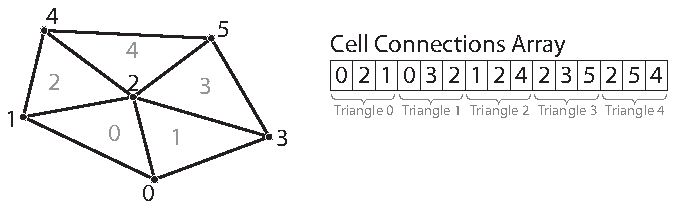
\includegraphics{images/CellConnections}
  \caption{The cell connection array for a simple triangle mesh.}
  \label{fig:CellConnections}
\end{figure}

The unstructured grid class is templated on the cell type
(\dax{CellTagHexahedron}, \dax{CellTagLine}, \dax{CellTagQuadrilateral},
\dax{CellTagTetrahedron}, \dax{CellTagTriangle}, \dax{CellTagVertex}, or
\dax{CellTagWedge}) the container for cell connections, the container for
the point coordinate array, and the device adapter. Its prototype looks as
follows.

\begin{daxexample}{Prototype for \protect\daxcont{UnstructuredGrid}.}
template <
    typename CellT,
    class CellConnectionsContainerControlTag = DAX_DEFAULT_ARRAY_CONTAINER_CONTROL_TAG,
    class PointsArrayContainerControlTag = DAX_DEFAULT_ARRAY_CONTAINER_CONTROL_TAG,
    class DeviceAdapterTag = DAX_DEFAULT_DEVICE_ADAPTER_TAG>
class UnstructuredGrid;
\end{daxexample}

The \daxcont{UnstructuredGrid} class provides the following features.
\begin{description}
\item[\textcode{CellTag}] A type that identifies what kind of cell is
  stored in this class. Always set to the first template parameter.
\item[\textcode{CellConnectionsType}] The type of the \daxcont{ArrayHandle}
  used to store cell connection indices.
\item[\textcode{PointCoordinatesType}] The type of the
  \daxcont{ArrayHandle} used to store point coordinates.
\item[\textcode{GetCellConnections}] A method used to get the array handle
  for the cell connections.
\item[\textcode{SetCellConnetions}] A method used to set the array handle
  for the cell connections.
\item[\textcode{GetPointCoordinates}] A method used to get the array handle
  for point coordinates.
\item[\textcode{SetPointCoordinates}] A method used to set the array handle
  for point coordinates.
\item[\textcode{ComputePointCoordinates}] A convenience method that takes a
  point index and returns the point coordinates at that index. The actual
  value is pulled from the point coordinates array.
\item[\textcode{GetNumberOfPoints}] A method that returns the number of
  points in the grid.
\item[\textcode{GetNumberOfCells}] A method that returns the number of
  cells in the grid.
\item[\textcode{TopologyStructExecution}] A memory copyable structure
  holding the state of the uniform grid that can be used in the execution
  environment.
\item[\textcode{TopologyStructConstExecution}] A read-only (const) form of
  \textcode{TopologyStructuExecution}.
\item[\textcode{PrepareForInput}] A method that returns a
  \textcode{TopologyStructConstExecution} object to pass to the execution
  environment. This method is typically only used internally within the Dax
  toolkit.
\item[\textcode{PrepareForOutput}] A method that returns a
  \textcode{TopologyStructExecution} object to pass to the execution
  environment. This method is typically only used internally within the Dax
  toolkit.
\end{description}

\index{unstructured~grid|)}

\subsection{Scheduling}
\label{sec:Scheduling}

\fix{Will the scheduler classes be changed in time?}

\subsection{Timers}
\label{sec:Timers}

\index{timer|(}

It is often the case that you need to measure the time it takes for an
operation to happen. This could be for performing measurements for
algorithm study or it could be to dynamically adjust scheduling.

Performing timing in a multi-threaded environment can be tricky because
operations happen asynchronously. In the Dax control environment timing is
simplified because the control environment operates on a single
thread. However, operations invoked in the execution environment may run
asynchronously to operations in the control environment.

To ensure that accurate timings can be made, Dax provides a \daxcont{Timer}
class that is templated on the device adapter to provide an accurate
measurement of operations that happen on the device. The timing starts with
the \textidentifier{Timer} is constructed. The time elapsed can be
retrieved with a call to the \textcode{GetElapsedTime} method. This method
will block until all operations in the execution environment complete so as
to return an accurate time. The timer can be restarted with a call to the
\textcode{Reset} method.

\begin{daxexample}{Using \protect\daxcont{Timer}.}
dax::cont::UniformGrid<> grid;
grid.SetExtent(dax::make_Id3(0, 0, 0), dax::make_Id3(99, 99, 99));
grid.SetOrigin(dax::make_Vector3(0.0, 0.0, 0.0));
grid.SetSpacing(dax::make_Vector3(1.0, 1.0, 1.0));

dax::cont::ArrayHandle<dax::Scalar> results;
dax::cont::Scheduler<> scheduler;
dax::worklet::Elevation worklet;

dax::cont::Timer<> timer;
scheduler.Invoke(worklet, grid.GetPointCoordinates(), results);
// This call makes sure data is pulled back to the host in a host/device architecture.
results.GetPortalConstControl();
dax::Scalar elapsedTime = timer.GetElapsedTime();

std::cout << "Time to run elevation: " << elapsedTime << std::endl;
\end{daxexample}

\index{timer|)}

\subsection{Error Handling}
\label{sec:ErrorHandlingControl}

\index{errors|(}

The Dax toolkit uses exceptions to report errors. All exceptions thrown by
Dax will be a subclass of \daxcont{Error}. For simple error reporting, it
is possible to simply catch a \daxcont{Error} and report the error message
string reported by the \textcode{GetMessage} method.

\begin{daxexample}{Simple error reporting.}
#include <dax/cont/Error.h>

int main(int argc, char **argv)
{
  try
    {
    // Do something cool with Dax
    // ...
    }
  catch (dax::cont::Error error)
    {
    std::cout << error.GetMessage() << std::endl;
    return 1;
    }
  return 0;
}
\end{daxexample}

There are two subclasses to \daxcont{Error}. These are
\daxcont{ErrorExecution} and \daxcont{ErrorControl}, and they represent
errors that happen in the respective execution and control environments.

Readers familiar with parallel programming will probably note the
difficulty in raising errors in multi-threaded execution like what happens
in the execution environment. In fact some devices, like CUDA devices, do
not support exceptions at all. Dax handles the error reporting in the
execution environment by flagging an error when it occurs and then throwing
an error in the control environment after all threads have terminated. This
means that the amount of execution that happens after an error is flagged
is indeterminate and any output values should be considered incorrect.

The \daxcont{ErrorControl} class is also broken down into several
subclasses that can be independently caught to handle different types of
errors. The following control errors exist and may be thrown.
\begin{description}
\item[\daxcont{ErrorControlAssert}] \index{assert} Thrown when an assertion
  fails, meaning a Dax operation reached an unexpected state. The header
  file \daxheader{dax/cont}{Assert.h} defines a macro named
  \daxmacro{DAX\_ASSERT\_CONT} that behaves much like the POSIX C assert
  macro except that a \textidentifier{ErrorControlAssert} is thrown rather
  than killing the application outright.
\item[\daxcont{ErrorControlBadValue}] Thrown when a Dax function or method
  encounters an invalid value that inhibits progress.
\item[\daxcont{ErrorControlInternal}] Thrown when Dax detects an internal
  state that should never be reached. This error usually indicates a bug in
  Dax or, at best, Dax failed to detect an invalid input it should have.
\item[\daxcont{ErrorControlOutOfMemory}] Thrown when a Dax function or
  method tries to allocate an array and fails.
\end{description}

\index{errors|)}

\index{device~adapter|(}

\subsection{Device Adapter Algorithms}
\label{sec:DeviceAdapterAlgorithms}

\index{device~adapter!algorithm|(}
\index{algorithm|(}

The Dax toolkit comes with the templated class
\daxcont{DeviceAdapterAlgorithm} that provides a set of algorithms that can
be invoked in the control environment and are run on the execution
environment. The template has a single argument that specifies the device
adapter tag.

\begin{daxexample}{Prototype for \protect\daxcont{DeviceAdapterAlgorithm}.}
namespace dax {
namespace cont {

template<class DeviceAdapterTag>
struct DeviceAdapterAlgorithm;

}
} // namespace dax::cont
\end{daxexample}

\textidentifier{DeviceAdapterAlgorithm} contains no state. It only has a
set of static methods that implement its algorithms. The following methods
are available.

\begin{description}
\item[\textcode{Copy}] \index{copy} Copies data from an input array to an
  output array. The copy takes place in the execution environment.
\item[\textcode{LowerBounds}] \index{lower~bounds} The
  \textcode{LowerBounds} method takes three arguments. The first argument
  is an \textidentifier{ArrayHandle} of sorted values. The second argument
  is another \textidentifier{ArrayHandle} of items to find in the first
  array. \textcode{LowerBounds} find the index of the first item that is
  greater than or equal to the target value, much like the
  \textcode{std::lower\_bound} STL algorithm. The results are returned in
  an \textidentifier{ArrayHandle} given in the third argument.

  There are two specializations of \textcode{LowerBounds}. The first takes
  an additional comparison function that defines the less-than
  operation. The second takes only two parameters. The first is an
  \textidentifier{ArrayHandle} of sorted \dax{Id}s and the second is an
  \textidentifier{ArrayHandle} of \dax{Id}s to find in the first list. The
  results are written back out to the second array. This second
  specialization is useful for inverting index maps.
\item[\textcode{ScanInclusive}] \index{scan!inclusive} The
  \textcode{ScanInclusive} method takes an input and an output
  \textidentifier{ArrayHandle} and performs a running sum on the input
  array. The first value in the output is the same as the first value in
  the input. The second value in the output is the sum of the first two
  values in the input. The third value in the output is the sum of the
  first three values of the input, and so on. \textcode{ScanInclusive}
  returns the sum of all values in the input.
\item[\textcode{ScanExclusive}] \index{scan!exclusive} The
  \textcode{ScanExclusive} method takes an input and an output
  \textidentifier{ArrayHandle} and performs a running sum on the input
  array. The first value in the output is always 0. The second value in the
  output is the same as the first value in the input. The third value in
  the output is the sum of the first two values in the input. The fourth
  value in the output is the sum of the first three values of the input,
  and so on. \textcode{ScanExclusive} returns the sum of all values in the
  input.
\item[\textcode{Schedule}] \index{schedule} The \textcode{Schedule} method
  takes a functor as its first argument and invokes it a number of times
  specified by the second argument. It should be assumed that each
  invocation of \textcode{Schedule} occurs on a separate thread although in
  practice there could be some thread sharing.

  There are two versions of the \textcode{Schedule} method. The first
  version takes a \dax{Id} and invokes the functor that number of
  times. The second version takes a \dax{Id3} and invokes the functor once
  for every entry in a 3D array of the given dimensions.

  The functor is expected to be an object with a const overloaded
  parentheses operator. The operator takes as a parameter the index of the
  invocation, which is either a \dax{Id} or a \dax{Id3} depending on what
  version of \textcode{Schedule} is being used. The functor must also
  provide a method named \textcode{SetErrorMessageBuffer} that accepts an
  argument of type \daxexecinternal{ErrorMessageBuffer}. If any errors
  occur during the invocations of the functor, it should call the
  \textcode{RaiseError} method of the
  \textidentifier{ErrorMessageBuffer}. That will cause the
  \textcode{Schedule} method to (eventually) throw a
  \daxcont{ErrorExecution} exception.
\item[\textcode{Sort}] \index{sort} The \textcode{Sort} method provides an
  unstable sort of an array. There are two forms of the \textcode{Sort}
  method. The first takes an \textidentifier{ArrayHandle} and sorts the
  values in place. The second takes an additional argument that is a
  functor that provides the comparison operation for the sort.
\item[\textcode{SortByKey}] \index{sort!by key} The \textcode{SortByKey}
  method works similarly to the \textcode{Sort} method except that it takes
  two \textidentifier{ArrayHandle}s: an array of keys and a corresponding
  array of values. The sort orders the array of keys in ascending values
  and also reorders the values so they remain paired with the same
  key. Like \textcode{Sort}, \textcode{SortByKey} has a version that sorts
  by the default less-than operator and a version that accepts a custom
  comparison functor.
\item[\textcode{StreamCompact}] \index{stream~compact} The
  \textcode{StreamCompact} method selectively removes values from an
  array. The first argument is an \textidentifier{ArrayHandle} to be
  compacted and the second argument is an \textidentifier{ArrayHandle} of
  equal size with flags indicating whether the corresponding input value is
  to be copied to the output. The third argument is an output
  \textidentifier{ArrayHandle} whose length is set to the number of true
  flags in the stencil and the passed values are put in order to the output
  array.

  There is also a second form of \textidentifier{StreamCompact} that only
  has the stencil and output as arguments. In this version, the output gets
  the corresponding index of where the input should be taken from.
\item[\textcode{Synchronize}] \index{synchronize} The
  \textidentifier{Synchronize} method waits for any asynchronous operations
  running on the device to complete and then returns.
\item[\textcode{Unique}] \index{unique} The \textcode{Unique} method
  removes all duplicate values in an \textidentifier{ArrayHandle}. The
  method will only find duplicates if they are adjacent to each other in
  the array. The easiest way to ensure that duplicate values are adjacent
  is to sort the array first.

  There are two versions of \textcode{Unique}. The first uses the equals
  operator to compare entries. The second accepts a binary functor to
  perform the comparisons.
\item[\textcode{UpperBounds}] \index{upper~bounds} The
  \textcode{UpperBounds} method takes three arguments. The first argument
  is an \textidentifier{ArrayHandle} of sorted values. The second argument
  is another \textidentifier{ArrayHandle} of items to find in the first
  array. \textcode{UpperBounds} find the index of the first item that is
  greater than to the target value, much like the
  \textcode{std::upper\_bound} STL algorithm. The results are returned in
  an \textidentifier{ArrayHandle} given in the third argument.

  There are two specializations of \textcode{UpperBounds}. The first takes
  an additional comparison function that defines the less-than
  operation. The second takes only two parameters. The first is an
  \textidentifier{ArrayHandle} of sorted \dax{Id}s and the second is an
  \textidentifier{ArrayHandle} of \dax{Id}s to find in the first list. The
  results are written back out to the second array. This second
  specialization is useful for inverting index maps.
\end{description}

\index{algorithm|)}
\index{device~adapter!algorithm|)}

\subsection{Implementing Device Adapters}
\label{sec:ImplementingDeviceAdapters}

The Dax toolkit comes with several implementations of device adapters so
that it may be ported to a variety of platforms. It is also possible to
provide new device adapters to support yet more devices, compilers, and
libraries. A new device adapter provides a tag, a class to manage arrays in
the execution environment, a collection of algorithms that run in the
execution environment, and (optionally) a timer.

Although not strictly necessary, the implementation of device adapters
within the Dax toolkit are divided into 3 header files with the names
\textfilename{DeviceAdapterTag\textasteriskcentered.h},
\textfilename{ArrayManagerExecution\textasteriskcentered.h} and
\textfilename{DeviceAdapterAlgorithm\textasteriskcentered.h}. The
\textfilename{DeviceAdapter\textasteriskcentered.h} that most code includes
is a trivial header that simply includes these other three files. For
example, the \daxheader{dax/tbb/cont}{DeviceAdapterTBB.h} for the Intel
Threading Building Blocks (TBB) device adapter simply contains the
following (with minutia like include guards removed).

\begin{daxexample}{Contents of \protect\daxheader{dax/tbb/cont}{DeviceAdapterTBB.h} file.}
#include <dax/tbb/cont/internal/DeviceAdapterTagTBB.h>
#include <dax/tbb/cont/internal/ArrayManagerExecutionTBB.h>
#include <dax/tbb/cont/internal/DeviceAdapterAlgorithmTBB.h>
\end{daxexample}

The reason the Dax toolkit breaks up the code for its device adapters this
way is that there is an interdependence between the implementation of each
device adapter and the mechanism to pick a default device adapter. Breaking
up the device adapter code in this way maintains an acyclic dependence among
header files.

\subsubsection{Tag}

The device adapter tag, as described in Section~\ref{sec:DeviceAdapterTag}
is a simple empty type that is used as a template parameter to identify the
device adapter. Every device adapter implementation provides one. The
device adapter tag is typically defined in an internal header file with a
prefix of \textfilename{DeviceAdapterTag}. Here is the implementation for
the TBB device adapter.

\begin{daxexample}{Implementation of the TBB device adapter tag.}
namespace dax {
namespace tbb {
namespace cont {

struct DeviceAdapterTagTBB {  };

}
}
} // namespace dax::tbb::cont
\end{daxexample}

\subsubsection{Array Manager Execution}

\index{device~adapter!array manager|(}
\index{array~manager~execution|(}
\index{execution~array~manager|(}

The Dax toolkit defines a template named
\daxcontinternal{ArrayManagerExecution} that is responsible for allocating
memory in the execution environment and copying data between the control
and execution environment. The execution array manager is typically defined
in an internal header file with a prefix of
\textfilename{ArrayManagerExecution}.

\begin{daxexample}{Prototype for \protect\daxcontinternal{ArrayManagerExecution}.}
namespace dax {
namespace cont {
namespace internal {

template<typename T, class ArrayContainerControlTag, class DeviceAdapterTag>
class ArrayManagerExecution;

}
}
} // namespace dax::cont::internal
\end{daxexample}

A device adapter must provide a partial specialization of
\textidentifier{ArrayManagerExecution} for its device adapter tag. The
implementation for \textidentifier{ArrayManagerExecution} is expected to
manage the resources for a single array, and it must provide the following
elements.

\begin{description}
\item[\textcode{ValueType}] A \textcode{typedef} of the type for each item
  in the array. This is the same type as the first template argument.
\item[\textcode{PortalType}] The type of an array portal that can be used
  in the execution environment to access the array.
\item[\textcode{PortalConstType}] A read-only (const) version of
  \textcode{PortalType}.
\item[\textcode{GetNumberOfValues}] A method that returns the number of
  values stored in the array. The results are undefined if the data has not
  been loaded or allocated.
\item[\textcode{LoadDataForInput}] A method that takes an array portal in
  the control environment, allocates a large enough array in the execution
  environment, and copies the data into that array. The data in the
  execution array is not expected to be changed. The allocated array can
  later be accessed via the \textcode{GetPortalConst} method.
\item[\textcode{LoadDataForInPlace}] A method that takes an array portal in
  the control environment, allocates a large enough array in the execution
  environment, and copies the data into that array. The data in the
  execution array is expected to be read and changed. The allocated array
  can later be accessed via the \textcode{GetPortal} and
  \textcode{GetPortalConst} methods.
\item[\textcode{AllocateArrayForOutput}] A method that takes an array
  container and a size and allocates an array in the execution environment
  of the specified size. The initial memory is uninitialized and can be
  accessed via the \textcode{GetPortal} method. The container argument can
  be used to allocate data when the control and execution share arrays, but
  this argument is often ignored.
\item[\textcode{RetrieveOutputData}] This method takes an array container,
  allocates memory in the control environment, and copies data from the
  execution environment into it.
\item[\textcode{CopyInto}] This method takes an STL-compatible iterator and
  copies data from the execution environment into it.
\item[\textcode{Shrink}] A method that adjusts the size of the array in the
  execution environment to something that is a smaller size. All the data
  up to the new length must remain valid. Typically, no memory is actually
  reallocated. Instead, a different end is marked.
\item[\textcode{GetPortal}] A method that returns an array portal
  that can be used in the execution environment. The portal was defined in
  either \textcode{LoadDataForInPlace} or
  \textcode{AllocateArrayForOutput}.
\item[\textcode{GetPortalConst}] A method that returns a read-only
  (const) array portal that can be used in the execution environment. The
  portal was defined in one of the load or allocate methods.
\item[\textcode{ReleaseResources}] A method that frees any resources
  (typically memory) in the execution environment.
\end{description}

Specializations of this template typically take on one of two forms. If the
control and execution environments have separate memory spaces, then this
class behaves by copying memory in methods such as
\textcode{PrepareForInput} and \textcode{RetrieveOutputData}. This might
require creating buffers in the control environment to efficiently move
data from control array portals.

However, if the control and execution environments share the same memory
space, the execution array manager can, and should, delegate all of its
operations to the \textidentifier{ArrayContainerControl} it is used
with. The Dax toolkit comes with a class called
\daxcontinternal{ArrayManagerExecutionShareWithControl} that provides the
implementation for an execution array manager that shares a memory space
with the control environment. In this case, making the
\textidentifier{ArrayManagerExecution} specialization be a trivial subclass
is sufficient. For example, here is the implementation of
\textidentifier{ArrayManagerExecution} for TBB.

\begin{daxexample}{Specialization of \textidentifier{ArrayManagerExecution} for TBB.}
#include <dax/tbb/cont/internal/DeviceAdapterTagTBB.h>

#include <dax/cont/internal/ArrayManagerExecution.h>
#include <dax/cont/internal/ArrayManagerExecutionShareWithControl.h>

namespace dax {
namespace cont {
namespace internal {

template <typename T, class ArrayContainerTag>
class ArrayManagerExecution
    <T, ArrayContainerTag, dax::tbb::cont::DeviceAdapterTagTBB>
    : public dax::cont::internal::ArrayManagerExecutionShareWithControl
        <T, ArrayContainerTag>
{
};

}
}
} // namespace dax::cont::internal
\end{daxexample}

\index{execution~array~manager|)}
\index{array~manager~execution|)}
\index{device~adapter!array manager|)}

\subsubsection{Algorithms}

\index{device~adapter!algorithm|(}
\index{algorithm|(}

A device adapter implementation must also provide a specialization of
\daxcont{DeviceAdapterAlgorithm}, which is documented in
Section~\ref{sec:DeviceAdapterAlgorithms}. The implementation for the
device adapter algorithms is typically placed in a header file with a
prefix of \textfilename{DeviceAdapterAlgorithm}.

Although there are many methods in
\textidentifier{DeviceAdapterAlgorithms}, it is seldom necessary to
implement them all. Instead, the Dax toolkit comes with
\daxcontinternal{DeviceAdapterAlgorithmGeneral} that provides generic
implementation for most of the required algorithms. By deriving the
specialization of \textidentifier{DeviceAdapterAlgorithm} from
\textidentifier{DeviceAdapterAlgorithmGeneral}, only the implementations
for \textcode{Schedule} and \textcode{Synchronize} need to be
implemented. All other algorithms can be derived from those.

That said, not all of the algorithms implemented in
\textidentifier{DeviceAdapterAlgorithmGeneral} are optimized for all types
of devices. Thus, it is worthwhile to provide algorithms optimized for the
specific device when possible. In particular, it is best to provide
specializations for the sort and scan algorithms.

The following example is a minimal implementation of the TBB device adapter
algorithms. The actual version that comes with the Dax toolkit contains
more enhancements.

\begin{daxexample}{Abbreviated implementation of \textidentifier{DeviceAdapterAlgorithm} for TBB.}
#include <dax/tbb/cont/internal/DeviceAdapterTagTBB.h>
#include <dax/tbb/cont/internal/ArrayManagerExecutionTBB.h>

#include <dax/cont/internal/DeviceAdapterAlgorithmGeneral.h>
#include <dax/exec/internal/IJKIndex.h>

#include <tbb/blocked_range.h>
#include <tbb/blocked_range3d.h>
#include <tbb/parallel_for.h>

namespace dax {
namespace cont {

template<>
struct DeviceAdapterAlgorithm<dax::tbb::cont::DeviceAdapterTagTBB> :
    dax::cont::internal::DeviceAdapterAlgorithmGeneral<
        DeviceAdapterAlgorithm<dax::tbb::cont::DeviceAdapterTagTBB>,
        dax::tbb::cont::DeviceAdapterTagTBB>
{
private:
  static const dax::Id TBB_GRAIN_SIZE = 128;

  template<class FunctorType>
  class ScheduleKernel
  {
  public:
    DAX_CONT_EXPORT ScheduleKernel(const FunctorType &functor)
      : Functor(functor)
    {  }

    DAX_CONT_EXPORT void SetErrorMessageBuffer(
        const dax::exec::internal::ErrorMessageBuffer &errorMessage)
    {
      this->ErrorMessage = errorMessage;
      this->Functor.SetErrorMessageBuffer(errorMessage);
    }

    DAX_EXEC_EXPORT
    void operator()(const ::tbb::blocked_range<dax::Id> &range) const {
      // The TBB device adapter causes array classes to be shared between
      // control and execution environment. This means that it is possible for
      // an exception to be thrown even though this is typically not allowed.
      // Throwing an exception from here is bad because there are several
      // simultaneous threads running. Get around the problem by catching the
      // error and setting the message buffer as expected.
      try
        {
        for (dax::Id index = range.begin(); index < range.end(); index++)
          {
          this->Functor(index);
          }
        }
      catch (dax::cont::Error error)
        {
        this->ErrorMessage.RaiseError(error.GetMessage().c_str());
        }
      catch (...)
        {
        this->ErrorMessage.RaiseError(
            "Unexpected error in execution environment.");
        }
    }
  private:
    FunctorType Functor;
    dax::exec::internal::ErrorMessageBuffer ErrorMessage;
  };

public:
  template<class FunctorType>
  DAX_CONT_EXPORT
  static void Schedule(FunctorType functor, dax::Id numInstances)
  {
    const dax::Id MESSAGE_SIZE = 1024;
    char errorString[MESSAGE_SIZE];
    errorString[0] = '\0';
    dax::exec::internal::ErrorMessageBuffer
        errorMessage(errorString, MESSAGE_SIZE);

    ScheduleKernel<FunctorType> kernel(functor);
    kernel.SetErrorMessageBuffer(errorMessage);

    ::tbb::blocked_range<dax::Id> range(0, numInstances, TBB_GRAIN_SIZE);

    ::tbb::parallel_for(range, kernel);

    if (errorMessage.IsErrorRaised())
      {
      throw dax::cont::ErrorExecution(errorString);
      }
  }

private:
  template<class FunctorType>
  class ScheduleKernelId3
  {
  public:
    DAX_CONT_EXPORT ScheduleKernelId3(const FunctorType &functor,
                                      const dax::Id3& dims)
      : Functor(functor),
        Dims(dims)
      {  }

    DAX_CONT_EXPORT void SetErrorMessageBuffer(
        const dax::exec::internal::ErrorMessageBuffer &errorMessage)
    {
      this->ErrorMessage = errorMessage;
      this->Functor.SetErrorMessageBuffer(errorMessage);
    }

    DAX_EXEC_EXPORT
    void operator()(const ::tbb::blocked_range3d<dax::Id> &range) const {
      try
        {
        dax::exec::internal::IJKIndex index(this->Dims);
        for( dax::Id k=range.pages().begin(); k!=range.pages().end(); ++k)
          {
          index.SetK(k);
          for( dax::Id j=range.rows().begin(); j!=range.rows().end(); ++j)
            {
            index.SetJ(j);
            for( dax::Id i=range.cols().begin(); i!=range.cols().end(); ++i)
              {
              index.SetI(i);
              this->Functor(index);
              }
            }
          }
        }
      catch (dax::cont::Error error)
        {
        this->ErrorMessage.RaiseError(error.GetMessage().c_str());
        }
      catch (...)
        {
        this->ErrorMessage.RaiseError(
            "Unexpected error in execution environment.");
        }
    }
  private:
    FunctorType Functor;
    dax::Id3 Dims;
    dax::exec::internal::ErrorMessageBuffer ErrorMessage;
  };

public:
  template<class FunctorType>
  DAX_CONT_EXPORT
  static void Schedule(FunctorType functor,
                       dax::Id3 rangeMax)
  {
    //we need to extract from the functor that uniform grid information
    const dax::Id MESSAGE_SIZE = 1024;
    char errorString[MESSAGE_SIZE];
    errorString[0] = '\0';
    dax::exec::internal::ErrorMessageBuffer
        errorMessage(errorString, MESSAGE_SIZE);

    //memory is generally setup in a way that iterating the first range
    //in the tightest loop has the best cache coherence.
    ::tbb::blocked_range3d<dax::Id> range(0, rangeMax[2],
                                          0, rangeMax[1],
                                          0, rangeMax[0]);

    ScheduleKernelId3<FunctorType> kernel(functor,rangeMax);
    kernel.SetErrorMessageBuffer(errorMessage);

    ::tbb::parallel_for(range, kernel);

    if (errorMessage.IsErrorRaised())
      {
      throw dax::cont::ErrorExecution(errorString);
      }
  }

  DAX_CONT_EXPORT static void Synchronize()
  {
    // Nothing to do. This device schedules all of its operations using a
    // split/join paradigm. This means that the if the control thread is
    // calling this method, then nothing should be running in the execution
    // environment.
  }

};

}
} // namespace dax::cont
\end{daxexample}

\index{algorithm|)}
\index{device~adapter!algorithm|)}

\subsubsection{Timer Implementation}

The Dax timer, described in Section~\ref{sec:Timers}, delegates to an
internal class named \daxcont{DeviceAdapterTimerImplementation}. The
interface for this class is the same as that for \daxcont{Timer}. A default
implementation of this templated class uses the system timer and the
\textcode{Synchronize} method in the device adapter algorithms.

However, some devices might provide alternate or better methods for
implementing timers. For example, the TBB library comes with a high
resolution timer that has better accuracy than the standard system
timers. Thus, the device adapter can optionally provide a specialization of
\textidentifier{DeviceAdapterTimerImplementation}, which is typically
placed in the same header file as the device adapter algorithms.

The following example is the implementation of the TBB timer
implementation.

\begin{daxexample}{Implementation of \textidentifier{DeviceAdapterTimerImplementation} for TBB.}
#include <dax/cont/DeviceAdapter.h>
#include <dax/tbb/cont/internal/DeviceAdapterTagTBB.h>

#include <tbb/tick_count.h>

namespace dax {
namespace cont {

template<>
class DeviceAdapterTimerImplementation<dax::tbb::cont::DeviceAdapterTagTBB>
{
public:
  DAX_CONT_EXPORT DeviceAdapterTimerImplementation()
  {
    this->Reset();
  }
  DAX_CONT_EXPORT void Reset()
  {
    dax::cont::DeviceAdapterAlgorithm<dax::tbb::cont::DeviceAdapterTagTBB>::Synchronize();
    this->StartTime = ::tbb::tick_count::now();
  }
  DAX_CONT_EXPORT dax::Scalar GetElapsedTime()
  {
    dax::cont::DeviceAdapterAlgorithm<dax::tbb::cont::DeviceAdapterTagTBB>::Synchronize();
    ::tbb::tick_count currentTime = ::tbb::tick_count::now();
    ::tbb::tick_count::interval_t elapsedTime = currentTime - this->StartTime;
    return static_cast<dax::Scalar>(elapsedTime.seconds());
  }

private:
  ::tbb::tick_count StartTime;
};

}
} // namespace dax::cont
\end{daxexample}

A word of warning about implementing timers. Although
\textcode{GetElapsedTime} returns a \dax{Scalar}, it is advisable to store
the internal timing in its native data format until the elapsed time is
recorded. This is because the times may be biased by a large value, and the
floating point number might not hold enough precision to get a precise
measurement between the start and end of the timer.

\subsubsection{Testing}

The implementation of a device adapter contains many components. To ensure
that all of its device adapters are working properly, the Dax toolkit
contains a complete test of all the components in
\daxheader{dax/cont/testing}{TestingDeviceAdapter.h}. Here is the
implementation for the TBB device adapter test, which plugs into the CMake
testing framework.

\begin{daxexample}{Test code for the TBB device adapter.}
#include <dax/tbb/cont/DeviceAdapterTBB.h>

#include <dax/cont/testing/TestingDeviceAdapter.h>

int UnitTestDeviceAdapterTBB(int, char *[])
{
  return dax::cont::testing::TestingDeviceAdapter
      <dax::tbb::cont::DeviceAdapterTagTBB>::Run();
}
\end{daxexample}

\index{device~adapter|)}

\index{control~environment|)}


\section{Execution Environment}
\label{sec:ExecutionEnvironment}

\index{execution~environment|(}

The execution environment is exposed to developers that write worklets for
different visualization algorithms. In addition to providing all the
mechanisms for building the worklet object itself, the execution
environment contains supporting code that can be useful to the
implementations of visualization algorithms.

The data structures in the execution environment provide information and
operations for a single element. This is in contrast to the control
environment, where data structures are built on arrays providing
information for large collections of data. These respective data structures
reflect the nature of the two environments. The control environment manages
the stores of data whereas the execution environment performs large
parallel processing through fine operations.

\subsection{Creating Worklets}
\label{sec:CreatingWorklets}

\index{worklet|(}

A worklet in Dax is most simply a functor that operates on an element of
data. Thus, it is a \textcode{class} or \textcode{struct} that has an
overloaded parenthesis operator (which must be declared \textcode{const}
for thread safety). It also must inherit from one of the predefined
abstract worker class, which will allow the Dax toolkit to load the correct
scheduler. Finally, it must declare a pair of
\index{signature}\keyterm{signatures} that define what information must be
presented when invoking the worklet and how this information gets passed to
each worklet invocation. Figure~\ref{fig:WorkletExampleAnnotated}
demonstrates all of the required components of a worklet.

\begin{figure}[htb]
  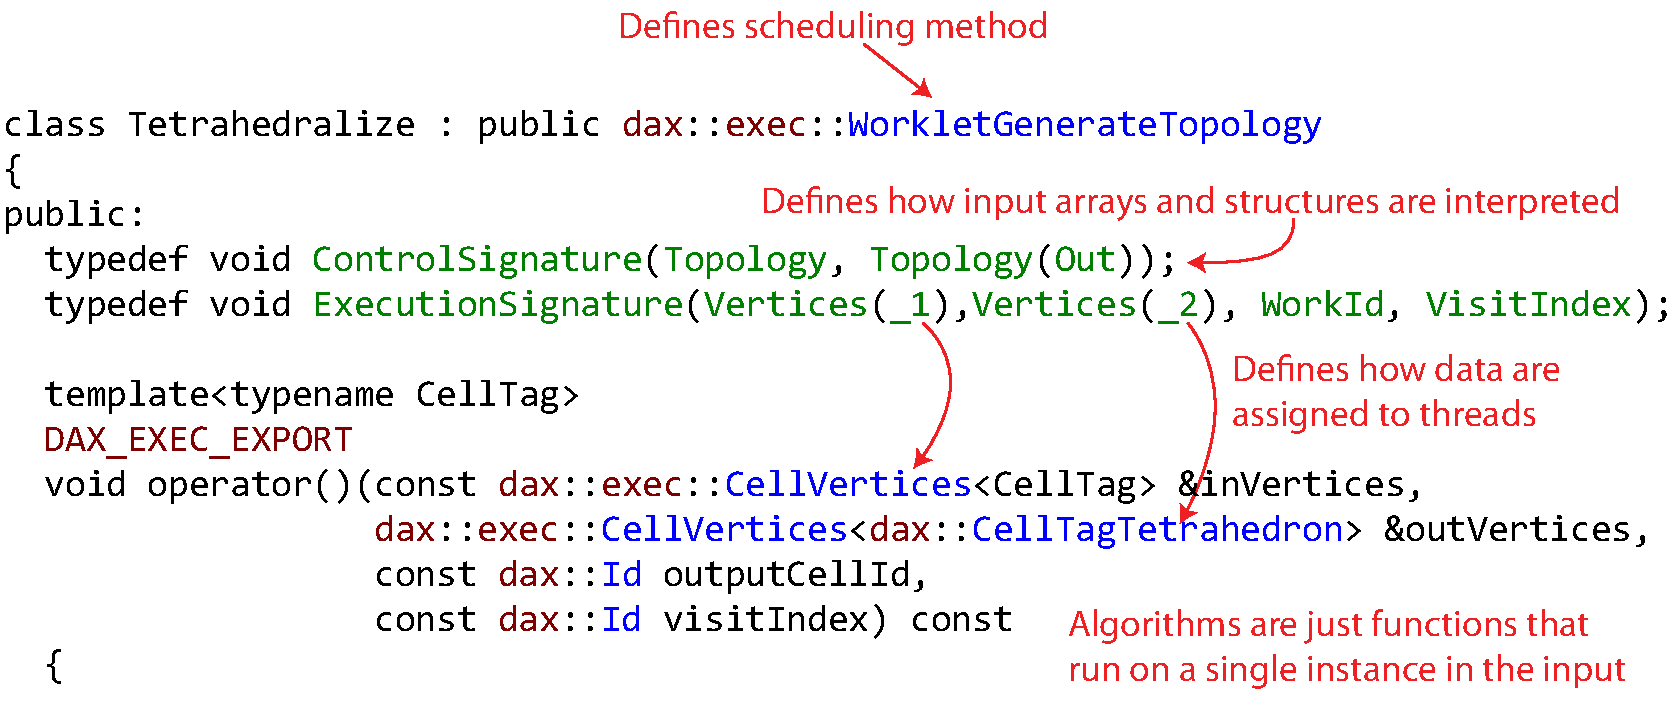
\includegraphics[width=\linewidth]{images/WorkletExampleAnnotated}
  \caption{Annotated example of a worklet declaration.}
  \label{fig:WorkletExampleAnnotated}
\end{figure}

\subsubsection{Control Signature}
\label{sec:ControlSignature}

\index{control~signature|(}
\index{signature!control|(}

The control signature of a worklet is the \textcode{typedef} of a function
prototype named \controlsignature. The function prototype matches the
calling specification used with the scheduler invoke function.

The return type of the function prototype is always \textcode{void} because
the scheduler invoke functions do not return values. The parameters of the
function prototype are \index{signature tags}\keyterm{tags} that identify
the type of data that is expected to be passed to invoke. For example, a
\sigtag{Field} tag declares that the worklet will operate on field data,
typically held in a \daxcont{ArrayHandle} whereas a \sigtag{Topology} tag
declares that the worklet will operate on a grid structure like those
documented in Section~\ref{sec:GridStructures}.

Tags can also have modifiers on them, which are attached with
parenthesis. For example, a \sigtag{Field} can be declared as either
\sigtagmod{Field}{Point} or \sigtagmod{Field}{Cell}. Likewise, a field
could be modified to be either \sigtag{In} (the default) or
\sigtag{Out}. \fix{Note that this method of using parenthesis to modify
  tags is likely to change as some compilers do not support it.}

The signature tags and their modifiers are described in greater detail in
the following section on worklet types.

\index{signature!control|)}
\index{control~signature|)}

\subsubsection{Execution Signature}
\label{sec:ExecutionSignature}

\index{execution~signature|(}
\index{signature!execution|(}

Like the control signature, the execution signature of a worklet is the
\textcode{typedef} of a function prototype named \executionsignature. The
function prototype must match the parenthesis operator in terms of arity
and argument semantics.

The arguments of the \executionsignature's function prototype are tags that
define where the data comes from. The most common tags are an underscore
followed by a number, such as \sigtagnum{1}, \sigtagnum{2}, etc. These
numbers refer back to the corresponding argument in the
\controlsignature. For example, \sigtagnum{1} means data from the first
control signature argument, \sigtagnum{2} means data from the second
control signature argument, etc.

Unlike the control signature, the execution signature optionally can
declare a return type if the parenthesis operator returns a value. If this
is the case, the return value should be one of the numeric tags
(i.e. \sigtagnum{1}, \sigtagnum{2}, etc.) to refer to one of the data
structures of the control signature. If the parenthesis operator does not
return a value, then \executionsignature should declare the return type as
\textcode{void}.

In addition to the numeric tags, there are other execution signature tags
to represent other types of data. For example, the \sigtag{WorkId} tag
identifies the instance of the worklet invocation. Each call to the worklet
function will have a unique \sigtag{WorkId}. Other such tags exist and are
described in the following section on worklet types where appropriate.

\index{signature!execution|)}
\index{execution~signature|)}

\subsubsection{Worklet Types}

\index{worklet types|(}

There are multiple worklet types provided by the Dax toolkit, each designed
to support a particular type of operation. This section will define each of
the worklet types, identify the generic superclass that a worklet instance
should derive, identify the signature tags and their meanings, and give an
example of the worklet in use.

\paragraph{Field Map}

\index{worklet types!field map|(}
\index{field map worklet|(}
\index{map field|see{field map worklet}}

A worklet deriving \daxexec{WorkletMapField} performs a basic mapping
operation that applies a function (the operator in the worklet) on all the
field values at a single point or cell and creates a new field value at
that same location. Although the intention is to operate on some variable
over the mesh, a \daxexec{WorkletMapField} actually be applied to any
array.

A field map worklet has only one type of \controlsignature tag:
\sigtag{Field}. This tag corresponds to a \daxcont{ArrayHandle} passed to
invoke, and each invocation of the worklet gets or sets a single value in
this array. The \sigtag{Field} tag can be modified to be either \sigtag{In}
(the default) or \sigtag{Out}.

A field map worklet supports the standard tags in its
\executionsignature. These are the numeric tags (e.g. \sigtagnum{1},
\sigtagnum{2}, etc.) and the \sigtag{WorkId} tag, which uniquely identifies
the invocation instance of the worklet.

Field maps most commonly perform basic calculator arithmetic, as
demonstrated in the following example.

\begin{daxexample}{Declaration and use of a field map worklet.}
#include <dax/exec/WorkletMapField.h>
#include <dax/cont/ArrayHandle.h>
#include <dax/cont/Scheduler.h>
#include <dax/math/VectorAnalysis.h>

class Magnitude : public dax::exec::WorkletMapField
{
public:
  typedef void ControlSignature(Field(In), Field(Out));
  typedef void ExecutionSignature(_1,_2);

  DAX_EXEC_EXPORT
  void operator()(const dax::Vector3 &inValue,
                  dax::Scalar &outValue) const
  {
    outValue = dax::math::Magnitude(inValue);
  }
};

DAX_CONT_EXPORT
dax::cont::ArrayHandle<dax::Scalar>
InvokeMagnitude(dax::cont::ArrayHandle<dax::Vector3> input)
{
  dax::cont::ArrayHandle<dax::Scalar> output;

  dax::cont::Scheduler<> scheduler;
  scheduler.Invoke(Magnitude(), input, output);

  return output;
}
\end{daxexample}

\index{field map worklet|)}
\index{worklet types!field map|)}

\paragraph{Cell Map}

\index{worklet types!cell map|(}
\index{cell map worklet|(}
\index{map cell|see{cell map worklet}}

A worklet deriving \daxexec{WorkletMapCell} performs a mapping operation
that applies a function (the operator in the worklet) on field values on a
single cell and creates a new field value at that location. The function
has access to all field values local to that cell. So if an input is a
point field, the operation will have access to all the values of that
field.

A cell map worklet supports the following tags in the parameters of its
\controlsignature.
\begin{description}
\item[\sigtag{Topology}] This tag corresponds to one of the grid structures
  described in Section~\ref{sec:GridStructures} passed to invoke that holds
  the topology on which to apply the map.

  If the \sigtag{Topology} argument is referenced with a numeric tag in the
  \executionsignature (e.g. with \sigtagnum{1}), then the worklet operator
  receives the cell-type tag (such as \dax{CellTagTriangle} or
  \dax{CellTagVoxel}). This is sometimes useful for specializing   based
  on the cell type, but usually unnecessary.

  If the \sigtag{Topology} argument is referenced by a \sigtag{Vertices}
  tag wrapping a numeric tag (e.g. with \sigtagmodnum{Vertices}{1}), then
  the worklet function is passed a \daxexec{CellVertices} object that
  contains the point indices for all the vertices of the cell.
\item[\sigtag{Field}] This tag corresponds to a \daxcont{ArrayHandle}
  passed to invoke that holds the sample values for a field at all points
  or all cells. The \sigtag{Field} tag can be modified to be either
  \sigtag{In} (the default) or \sigtag{Out}. Input \sigtag{Field} tags can
  be further modified to be attached to \sigtag{Point}s or
  \sigtag{Cell}s. The size of the input \daxcont{ArrayHandle} must match
  the number of points or cells in the grid structure passed in as a
  \sigtag{Topology} argument.  Output fields are always attached to the
  cells, and the corresponding \daxcont{ArrayHandle} will be resized as
  necessary.

  A cell field has a one-to-one mapping between \daxcont{ArrayHandle}
  entries and worklet function parameters. Thus, when the
  \executionsignature references a \controlsignature \sigtag{Field}
  parameter (e.g. with \sigtagnum{2}), the parameter is the same as the
  basic type as the values in the array (typically something like
  \dax{Scalar} or \dax{Vector3}).

  A point field has a many-to-one mapping between \daxcont{ArrayHandle}
  entries and worklet function parameters because each cell can touch
  multiple points. So when a \daxcont{ArrayHandle} is translated to the
  worklet invocation, its values get passed in a \daxexec{CellField}
  object, which behaves like a \dax{Tuple} with a size matching the number
  of vertices in a cell.
\end{description}

A cell map worklet supports the following tags in the parameters of its
\executionsignature.
\begin{description}
\item[\sigtagnum{1}, \sigtagnum{2},$\ldots$] These reference the
  corresponding parameter in the \controlsignature.
\item[\sigtag{Vertices}] When modified by one of the numeric tags
  (e.g. \sigtagmodnum{Vertices}{1}), passes a \daxexec{CellVertices} to the
  worklet representing the point indices for each vertex of the cell.
\item[\sigtag{WorkId}] Produces a \dax{Id} that uniquely identifies the
  invocation instance of the worklet.
\end{description}

Cell maps most commonly perform operations on interpolated fields. They
often use the cell operations provided by the Dax toolkit and described in
Section~\ref{sec:CellsAndOperations}. The following example shows a cell
map worklet that simply averages all the point values it touches. A more
serious worklet would probably perform interpolations, derivatives, or
integrations over the cell.

\begin{daxexample}{Declaration and use of a cell map worklet.}
#include <dax/exec/WorkletMapCell.h>

#include <dax/exec/CellField.h>

#include <dax/cont/Scheduler.h>
#include <dax/cont/ArrayHandle.h>
#include <dax/cont/UniformGrid.h>

class CellAverage : public dax::exec::WorkletMapCell
{
public:
  typedef void ControlSignature(Topology, Field(Point), Field(Out));
  typedef _3 ExecutionSignature(_1,_2);

  template<class CellTag>
  DAX_EXEC_EXPORT
  dax::Scalar operator()(
    CellTag, const dax::exec::CellField<dax::Scalar,CellTag> &values) const
  {
    dax::Scalar sum = values[0];
    for (int index = 1; index < values.NUM_VERTICES; index++)
      {
      sum += values[index];
      }
    return sum/values.NUM_VERTICES;
  }
};

DAX_CONT_EXPORT
void InvokeCellAverage()
{
  const dax::Id DIM = 100;

  // Make a grid structure.
  dax::cont::UniformGrid<> grid;
  grid.SetExtent(dax::make_Id3(0, 0, 0), dax::make_Id3(DIM-1, DIM-1, DIM-1));

  // Make input.
  // (A real application would make more interesting data and do it more efficiently.)
  dax::Scalar inputBuffer[DIM*DIM*DIM];
  for (dax::Id index = 0; index < DIM*DIM*DIM; index++)
    {
    inputBuffer[index] = index;
    }
  dax::cont::ArrayHandle<dax::Scalar> input =
      dax::cont::make_ArrayHandle(inputBuffer, DIM*DIM*DIM);

  dax::cont::ArrayHandle<dax::Scalar> output;

  dax::cont::Scheduler<> scheduler;
  scheduler.Invoke(CellAverage(), grid, input, output);

  // Do something with output.
}

\end{daxexample}

\index{cell map worklet|)}
\index{worklet types!cell map|)}

\paragraph{Generate Topology}

\index{worklet types!generate topology|(}
\index{generate topology worklet|(}

A worklet deriving from \daxexec{WorkletGenerateTopology} generates a cell
connectivity. When invoked, the scheduler is given an array containing the
number of output cells derived from each input cell. Each invocation of a
\daxexec{WorkletGenerateTopology} produces exactly one cell, so the
scheduler then invokes the generate topology worklet multiple times per
cell if multiple cells are derived.

A generate topology worklet supports the following tags in the parameters
of its \controlsignature.
\begin{description}
\item[\sigtag{Topology}] This tag corresponds to one of the grid structures
  described in Section~\ref{sec:GridStructures} passed to invoke that holds
  the topology on which to derive a new topology or to write the new
  topology into. The \sigtag{Topology} tag can be modified to be either
  \sigtag{In} (the default) or \sigtag{Out}.

  If the \sigtag{Topology} argument is referenced with a numeric tag in the
  \executionsignature (e.g. with \sigtagnum{1}), then the worklet operator
  receives the cell-type tag (such as \dax{CellTagTriangle} or
  \dax{CellTagVoxel}). This is sometimes useful for specializing   based
  on the cell type, but usually unnecessary.

  If the \sigtag{Topology} argument is referenced by a \sigtag{Vertices}
  tag wrapping a numeric tag (e.g. with \sigtagmodnum{Vertices}{1}), then
  the worklet function is passed a \daxexec{CellVertices} object that
  contains the point indices for all the vertices of the cell.
\item[\sigtag{Field}] This tag corresponds to a \daxcont{ArrayHandle}
  passed to invoke that holds the sample values for a field at all points
  or all cells. All fields for generate topology worklets are input. The
  \sigtag{Field} tag can be modified to be attached to \sigtag{Point}s or
  \sigtag{Cell}s. The size of the \daxcont{ArrayHandle} must match the
  number of points or cells in the grid structure passed in as a
  \sigtag{Topology} argument.

  A cell field has a one-to-one mapping between \daxcont{ArrayHandle}
  entries and worklet function parameters. Thus, when the
  \executionsignature references a \controlsignature \sigtag{Field}
  parameter (e.g. with \sigtagnum{2}), the parameter is the same as the
  basic type as the values in the array (typically something like
  \dax{Scalar} or \dax{Vector3}).

  A point field has a many-to-one mapping between \daxcont{ArrayHandle}
  entries and worklet function parameters because each cell can touch
  multiple points. So when a \daxcont{ArrayHandle} is translated to the
  worklet invocation, its values get passed in a \daxexec{CellField}
  object, which behaves like a \dax{Tuple} with a size matching the number
  of vertices in a cell.
\end{description}

A generate topology worklet supports the following tags in the parameters
of its \executionsignature.
\begin{description}
\item[\sigtagnum{1}, \sigtagnum{2},$\ldots$] These reference the
  corresponding parameter in the \controlsignature.
\item[\sigtag{Vertices}] When modified by one of the numeric tags
  (e.g. \sigtagmodnum{Vertices}{1}), passes a \daxexec{CellVertices} to the
  worklet representing the point indices for each vertex of the cell. The
  numeric tag must point to a \controlsignature parameter of type
  \sigtag{Topology}.
\item[\sigtag{VisitId}] Produces a \dax{Id} that uniquely identifies the
  invocation instance for the particular cell being visited. For example,
  if dividing hexahedra into tetrahedra, each hexahedra produces 5 or 6
  tetrahedra, but each invocation of the generate topology worklet
  generates just one of this. The \sigtag{VisitId} identifies which of the
  tetrahedra to produce.
\item[\sigtag{WorkId}] Produces a \dax{Id} that uniquely identifies the
  invocation instance of the worklet.
\end{description}

Generate topology operations are used when one topology is derived from
another's points. A generate topology is often proceeded by a field map or
cell map that counts how many cells will be derived from each input
cell. These counts are stored in an array and held in a
\daxcont{GenerateTopology} object that wraps the worklet and is passed to
the scheduler. \fix{This should change soon.}

The following example converts a uniform grid of voxels into the a
collection of quadrilaterals that make up the faces. The worklet leverages
the implicit topology of a uniform grid to ensure that each face is
represented exactly once.

\begin{daxexample}{Declaration and use of a generate topology worklet.}
#include <dax/exec/WorkletGenerateTopology.h>

#include <dax/Extent.h>

#include <dax/exec/CellVertices.h>
#include <dax/exec/WorkletMapCell.h>

#include <dax/cont/ArrayHandle.h>
#include <dax/cont/GenerateTopology.h>
#include <dax/cont/Scheduler.h>
#include <dax/cont/UniformGrid.h>
#include <dax/cont/UnstructuredGrid.h>

DAX_EXEC_CONSTANT_EXPORT
const unsigned char VoxelFaces[6][4] = {
  { 0, 3, 7, 4 },
  { 0, 4, 5, 1 },
  { 0, 1, 2, 3 },
  { 1, 2, 6, 5 },
  { 2, 3, 7, 6 },
  { 4, 5, 6, 7 }
};

class CountFaceOut : public dax::exec::WorkletMapCell
{
public:
  typedef void ControlSignature(Topology, Field(Out), Field(Out));
  typedef _3 ExecutionSignature(WorkId, _2);

  DAX_CONT_EXPORT
  CountFaceOut(dax::Id3 dimensions) : Dimensions(dimensions) {  }

  DAX_EXEC_EXPORT
  dax::Id operator()(dax::Id workId, dax::Tuple<unsigned char,6> &faceToOutput) const
  {
    dax::Id3 index3D;
    dax::Id flatIndex = workId;
    for (i = 0; i < 3; i++)
      {
      index3D[i] = flatIndex % this->Dimensions[i];
      flatIndex /= this->Dimensions[i];
      }

    dax::Id count = 0;
    // First three faces output on all cells.
    faceToOutput[count] = 0;  count++;
    faceToOutput[count] = 1;  count++;
    faceToOutput[count] = 2;  count++;

    // Second three faces output only on cells at maximum boundary.
    if (flatIndex[0] == this->Dimensions[0]-1) { faceToOutput[count] = 3;  count++; }
    if (flatIndex[1] == this->Dimensions[1]-1) { faceToOutput[count] = 4;  count++; }
    if (flatIndex[2] == this->Dimensions[2]-1) { faceToOutput[count] = 5;  count++; }

    return count;
  }

private:
  dax::Id3 Dimensions;
};

class ExtractFace : public dax::exec::WorkletGenerateTopology
{
public:
  typedef void ControlSignature(Topology, Topology(Out), Field);
  typedef void ExecutionSignature(Vertices(_1), Vertices(_2), _3, VisitIndex);

  DAX_EXEC_EXPORT
  void operator()(const dax::exec::CellVertices<dax::CellTagVoxel> &inVertices,
                  dax::exec::CellVertices<dax::CellTagQuadrilateral> &outVertices,
                  const dax::Tuple<unsigned char,6> outputFaces,
                  dax::Id visitIndex) const
  {
    unsigned char faceId = outputFaces[visitIndex];
    outVertices[0] = inVertices[VoxelFaces[faceId][0]];
    outVertices[1] = inVertices[VoxelFaces[faceId][1]];
    outVertices[2] = inVertices[VoxelFaces[faceId][2]];
    outVertices[3] = inVertices[VoxelFaces[faceId][3]];
  }
};

DAX_CONT_EXPORT
dax::cont::UnstructuredGrid<dax::CellTagQuadrilateral>
InvokeExtraceFaces(const dax::cont::UniformGrid<> &inputGrid)
{
  dax::Id3 dimensions = dax::extentCellDimensions(inputGrid.GetExtent());

  dax::cont::ArrayHandle<dax::Tuple<unsigned char,6> > faces;
  dax::cont::ArrayHandle<dax::Id> counts;

  dax::cont::Scheduler<> scheduler;
  scheduler.Invoke(CountFaceOut(dimensions), inputGrid, faces, counts);

  dax::cont::UnstructuredGrid<dax::CellTagQuadrilateral> outputGrid;

  dax::cont::GenerateTopology<ExtractFace> extractFace(counts);
  extractFace.SetRemoveDuplicatePoints(false); // All points will be used.
  scheduler.Invoke(extractFace, inputGrid, outputGrid, faces);

  return outputGrid;
}
\end{daxexample}

\index{generate topology worklet|)}
\index{worklet types!generate topology|)}

\paragraph{Interpolated Cell}

\index{worklet types!interpolated cell|(}
\index{interpolated cell worklet|(}

A worklet deriving from \daxexec{WorkletInterpolatedCell} generates a new
geometry comprising both new points at new coordinates and cell connections
among those points. When invoked, the scheduler is given an array
containing the number of cells produced. (The cell type must be
homogeneous.) Each invocation of a \daxexec{WorkletInterpolatedCell}
produces exactly one cell and its associated points, so the scheduler then
invokes the interpolated cell worklet multiple times per cell if multiple
cells are derived.

An interpolated cell worklet supports the following tags in the parameters
of its \controlsignature.
\begin{description}
\item[\sigtag{Topology}] This tag corresponds to one of the grid structures
  described in Section~\ref{sec:GridStructures} passed to invoke that holds
  the topology on which to derive a new topology.

  If the \sigtag{Topology} argument is referenced with a numeric tag in the
  \executionsignature (e.g. with \sigtagnum{1}), then the worklet operator
  receives the cell-type tag (such as \dax{CellTagTriangle} or
  \dax{CellTagVoxel}). This is sometimes useful for specializing   based
  on the cell type, but usually unnecessary.

  If the \sigtag{Topology} argument is referenced by a \sigtag{Vertices}
  tag wrapping a numeric tag (e.g. with \sigtagmodnum{Vertices}{1}), then
  the worklet function is passed a \daxexec{CellVertices} object that
  contains the point indices for all the vertices of the cell.
\item[\sigtag{Geometry}] This tag corresponds to one of the grid structures
  described in Section~\ref{sec:GridStructures} passed to
  invoke. Parameters of this type access the full geometry of the grid
  including both point locations and cell connections. The
  \sigtag{Geometry} tag is always used in the output of an interpolated
  cell worklet, and so should be modified with \sigtag{Out}.

  When the \executionsignature references a \controlsignature
  \sigtag{Geometry} parameter (e.g. with \sigtagnum{2}), the parameter is a
  \daxexec{InterpolatedCellPoints} object. The worklet operator should pass
  this parameter by reference so that it may be filled and the results
  returned.
\item[\sigtag{Field}] This tag corresponds to a \daxcont{ArrayHandle}
  passed to invoke that holds the sample values for a field at all points
  or all cells. All fields for generate topology worklets are input. The
  \sigtag{Field} tag can be modified to be attached to \sigtag{Point}s or
  \sigtag{Cell}s. The size of the \daxcont{ArrayHandle} must match the
  number of points or cells in the grid structure passed in as a
  \sigtag{Topology} argument.

  A cell field has a one-to-one mapping between \daxcont{ArrayHandle}
  entries and worklet function parameters. Thus, when the
  \executionsignature references a \controlsignature \sigtag{Field}
  parameter (e.g. with \sigtagnum{2}), the parameter is the same as the
  basic type as the values in the array (typically something like
  \dax{Scalar} or \dax{Vector3}).

  A point field has a many-to-one mapping between \daxcont{ArrayHandle}
  entries and worklet function parameters because each cell can touch
  multiple points. So when a \daxcont{ArrayHandle} is translated to the
  worklet invocation, its values get passed in a \daxexec{CellField}
  object, which behaves like a \dax{Tuple} with a size matching the number
  of vertices in a cell.
\end{description}

An interpolated cell worklet supports the following tags in the parameters
of its \executionsignature.
\begin{description}
\item[\sigtagnum{1}, \sigtagnum{2},$\ldots$] These reference the
  corresponding parameter in the \controlsignature.
\item[\sigtag{Vertices}] When modified by one of the numeric tags
  (e.g. \sigtagmodnum{Vertices}{1}), passes a \daxexec{CellVertices} to the
  worklet representing the point indices for each vertex of the cell. The
  numeric tag must point to a \controlsignature parameter of type
  \sigtag{Topology}.
\item[\sigtag{VisitId}] Produces a \dax{Id} that uniquely identifies the
  invocation instance for the particular cell being visited. For example,
  if dividing hexahedra into tetrahedra, each hexahedra produces 5 or 6
  tetrahedra, but each invocation of the generate topology worklet
  generates just one of this. The \sigtag{VisitId} identifies which of the
  tetrahedra to produce.
\item[\sigtag{WorkId}] Produces a \dax{Id} that uniquely identifies the
  invocation instance of the worklet.
\end{description}

Interpolated cell operations are used when one topology is derived from
another, but the new topology can build cells in unconstrained ways. An
interpolated cell is often proceeded by a field map or cell map that counts
how many cells will be derived from each input cell. These counts are
stored in an array and held in a \daxcont{GenerateInterpolatedCells} class
that wraps the worklet and is passed to the scheduler. \fix{This should
  change soon.}

The following example performs a slice on a uniform grid using a plane that
is aligned with the x axis (parallel with the y-z plane). With these
constraints, we know that the intersection of every cell will be a
quadrilateral.

\begin{daxexample}{Declaration and use of an interpolated cell worklet.}
#include <dax/exec/WorkletInterpolatedCell.h>

#include <dax/exec/CellField.h>
#include <dax/exec/CellVertices.h>
#include <dax/exec/InterpolatedCellPoints.h>
#include <dax/exec/WorkletMapCell.h>

#include <dax/cont/ArrayHandle.h>
#include <dax/cont/GenerateInterpolatedCells.h>
#include <dax/cont/Scheduler.h>
#include <dax/cont/UniformGrid.h>
#include <dax/cont/UnstructuredGrid.h>

class CountXSliceOut : public dax::exec::WorkletMapCell
{
public:
  typedef void ControlSignature(Topology, Field(Point), Field(Out));
  typedef _3 ExecutionSignature(_2);

  DAX_CONT_EXPORT
  CountXSliceOut(dax::Scalar xIntercept) : XIntercept(xIntercept) {  }

  DAX_EXEC_EXPORT
  dax::Id operator()(
      const dax::exec::CellField<dax::Vector3, dax::CellTagVoxel> &pointCoordinates) const
  {
    dax::Scalar minX = pointCoordinates[0][0];
    dax::Scalar maxX = pointCoordinates[6][0];

    return ((minX <= this->XIntercept) && (this->XIntercept < maxX)) ? 1 : 0;
  }

private:
  dax::Scalar XIntercept;
};

class XSlice : public dax::exec::WorkletInterpolatedCell
{
public:
  typedef void ControlSignature(Topology, Geometry(Out), Field(Point));
  typedef void ExecutionSignature(Vertices(_1), _2, _3);

  DAX_CONT_EXPORT
  XSlice(dax::Scalar xIntercept) : XIntercept(xIntercept) {  }

  DAX_EXEC_EXPORT
  void operator()(
      const dax::exec::CellVertices<dax::CellTagVoxel> &inVertices,
      dax::exec::InterpolatedCellPoints<dax::CellTagQuadrilateral> &outVertices,
      const dax::exec::CellField<dax::Vector3, dax::CellTagVoxel> &pointCoordinates) const
  {
    dax::Scalar minX = pointCoordinates[0][0];
    dax::Scalar maxX = pointCoordinates[6][0];
    dax::Scalar interpolant = (this->XIntercept - minX)/(maxX - minX);

    outVertices.SetInterpolationPoint(0, inVertices[0], inVertices[1], interpolant);
    outVertices.SetInterpolationPoint(1, inVertices[3], inVertices[2], interpolant);
    outVertices.SetInterpolationPoint(2, inVertices[4], inVertices[5], interpolant);
    outVertices.SetInterpolationPoint(3, inVertices[7], inVertices[6], interpolant);
  }

private:
  dax::Scalar XIntercept;
};

DAX_CONT_EXPORT
dax::cont::UnstructuredGrid<dax::CellTagQuadrilateral>
InvokeXSlice(const dax::cont::UniformGrid<> &inputGrid, dax::Scalar xIntercept)
{
  dax::cont::ArrayHandle<dax::Id> counts;

  dax::cont::Scheduler<> scheduler;
  scheduler.Invoke(CountXSliceOut(xIntercept),
                   inputGrid,
                   inputGrid.GetPointCoordinates(),
                   counts);

  dax::cont::UnstructuredGrid<dax::CellTagQuadrilateral> outputGrid;

  dax::cont::GenerateInterpolatedCells<XSlice> slicer(count, XSlice(xIntercept));
  extractFace.SetRemoveDuplicatePoints(true);
  scheduler.Invoke(slicer, inputGrid, outputGrid, inputGrid.GetPointCoordinates());

  return outputGrid;
}
\end{daxexample}

\index{interpolated cell worklet|)}
\index{worklet types!interpolated cell|)}

\paragraph{Generate Keys and Values}

\index{worklet types!generate keys and values|(}
\index{generate keys and values worklet|(}

A worklet deriving from \daxexec{WorkletGenerateKeysValues}, which is
designed to be used in conjunction with the reduce keys and values worklet,
is an experimental type of worklet that can be applied to a variety of
visualization algorithms. They allow an algorithm with a lot of
interdependence to operate with lots of concurrency by storing and
deferring the interdependent operation.

In operation the generate keys and values worklet works very much like a
cell map worklet except that it is able to produce a variable amount of
field values per cell. Each invocation of a
\daxexec{WorkletGenerateKeysValues} generates one set of keys and values,
so the scheduler then invokes the worklet multiple times per cell if
multiple key-value sets are needed.

Although the \daxexec{WorkletGenerateKeysValues} worklet is expected to
generate keys and values which have distinct semantics, the worklet itself
does not distinguish between them. Instead, both keys and values are simply
considered output fields.

A generate keys and values worklet supports the following tags in the
parameters of its \controlsignature.
\begin{description}
\item[\sigtag{Topology}] This tag corresponds to one of the grid structures
  described in Section~\ref{sec:GridStructures} passed to invoke that holds
  the topology on which to apply the map.

  If the \sigtag{Topology} argument is referenced with a numeric tag in the
  \executionsignature (e.g. with \sigtagnum{1}), then the worklet operator
  receives the cell-type tag (such as \dax{CellTagTriangle} or
  \dax{CellTagVoxel}). This is sometimes useful for specializing   based
  on the cell type, but usually unnecessary.

  If the \sigtag{Topology} argument is referenced by a \sigtag{Vertices}
  tag wrapping a numeric tag (e.g. with \sigtagmodnum{Vertices}{1}), then
  the worklet function is passed a \daxexec{CellVertices} object that
  contains the point indices for all the vertices of the cell.
\item[\sigtag{Field}] This tag corresponds to a \daxcont{ArrayHandle}
  passed to invoke that holds the sample values for a field at all points
  or all cells. The \sigtag{Field} tag can be modified to be either
  \sigtag{In} (the default) or \sigtag{Out}. Input \sigtag{Field} tags can
  be further modified to be attached to \sigtag{Point}s or
  \sigtag{Cell}s. The size of the input \daxcont{ArrayHandle} must match
  the number of points or cells in the grid structure passed in as a
  \sigtag{Topology} argument.  Output fields are always attached to the
  cells, and the corresponding \daxcont{ArrayHandle} will be resized as
  necessary.

  A cell field has a one-to-one mapping between \daxcont{ArrayHandle}
  entries and worklet function parameters. Thus, when the
  \executionsignature references a \controlsignature \sigtag{Field}
  parameter (e.g. with \sigtagnum{2}), the parameter is the same as the
  basic type as the values in the array (typically something like
  \dax{Scalar} or \dax{Vector3}).

  A point field has a many-to-one mapping between \daxcont{ArrayHandle}
  entries and worklet function parameters because each cell can touch
  multiple points. So when a \daxcont{ArrayHandle} is translated to the
  worklet invocation, its values get passed in a \daxexec{CellField}
  object, which behaves like a \dax{Tuple} with a size matching the number
  of vertices in a cell.
\end{description}

A generate keys and values worklet supports the following tags in the
parameters of its \executionsignature.
\begin{description}
\item[\sigtagnum{1}, \sigtagnum{2},$\ldots$] These reference the
  corresponding parameter in the \controlsignature.
\item[\sigtag{Vertices}] When modified by one of the numeric tags
  (e.g. \sigtagmodnum{Vertices}{1}), passes a \daxexec{CellVertices} to the
  worklet representing the point indices for each vertex of the cell.
\item[\sigtag{VisitId}] Produces a \dax{Id} that uniquely identifies the
  invocation instance for the particular cell being visited. For example,
  if performing an operation on all cell values incident to a point, these
  values can be collected by generating keys on the point index. Each cell
  will generate one key-value per vertex, and the \sigtag{VisitId}
  identifies which of the vertices to key on.
\item[\sigtag{WorkId}] Produces a \dax{Id} that uniquely identifies the
  invocation instance of the worklet.
\end{description}

When invoking, the scheduler needs to know how many key-values to produce
per cell. These counts are stored in an array hand held in a
\daxcont{GenerateKeysValues} object that wraps the worklet and is passed to
the scheduler. \fix{This should change soon.} If all cells produced the
same number of key-values, then the implicit \daxcont{ArrayHandleConstant}
can be used.

An example of defining and using a generate keys and values worklet is
given in the next section in conjunction with a reduce keys and values
worklet.

\index{generate keys and values worklet|)}
\index{worklet types!generate keys and values|)}

\paragraph{Reduce Keys and Values}

\index{worklet types!reduce keys and values|(}
\index{reduce keys and values worklet|(}

A worklet deriving from \daxexec{WorkletReduceKeysValues} is an
experimental type of worklet that can be applied to a variety of
visualization algorithms. They allow an algorithm with a lot of
interdependence to operate with lots of concurrency by storing and
deferring the interdependent operation.

When invoking a \daxexec{WorkletReduceKeysValues}, the scheduler groups
values based on their associated keys and calls a single instance of the
worklet for every unique key given. The keys are given to the scheduler
through a \daxcont{ReduceKeysValues} object that wraps the
worklet. \fix{This should change soon.} The values are passed as parameters
and are automatically grouped by key before being passed to the worklet.

A reduce keys and values worklet supports only one tags in the parameters
of its \controlsignature: \sigtag{Value}. A \sigtag{Value} corresponds to a
\daxcont{ArrayHandle} passed into the invoke method. The \sigtag{Value} tag
can be modified to be either \sigtag{In} or \sigtag{Out}. The semantics of
the input and output values are a bit different.

A \sigtagmod{Value}{In} corresponds to an input \daxcont{ArrayHandle} with
the same number of entries as there are keys. This type of parameter must
be referenced in the \executionsignature using the \sigtag{KeyGroup} tag
modified by the numeric tag (for example, \sigtagmodnum{KeyGroup}{1}). The
values of the group are passed in through a \daxexec{KeyGroup} object. A
\textidentifier{KeyGroup} object has a \textcode{GetNumberOfValues} method
that returns the number of values in the group and a \textcode{Get} method
that retrieves the value with a given group
index. \textidentifier{KeyGroup} objects also have an overloaded bracket
operator so that they can be referenced like an array or tuple.

A \sigtagmod{Value}{Out} corresponds to an output
\daxcont{ArrayHandle}. The scheduler will resize this array to the number
of unique keys, and each instance of the worklet produces one entry into
this array. This type of parameter is referenced in the \executionsignature
simply with a numeric tag (such as \sigtagnum{2}).

The following example shows a pair of generate keys-values and reduce
keys-values worklets that, for each point, simply averages all the cell
values it touches.

\begin{daxexample}{Declaration and use of generation and reduction of keys and values.}
#include <dax/exec/WorkletGenerateKeysValues.h>
#include <dax/exec/WorkletReduceKeysValues.h>

#include <dax/CellTraits.h>

#include <dax/exec/CellVertices.h>

#include <dax/cont/ArrayHandle.h>
#include <dax/cont/ArrayHandleConstant.h>
#include <dax/cont/GenerateKeysValues.h>
#include <dax/cont/ReduceKeysValues.h>
#include <dax/cont/Scheduler.h>
#include <dax/cont/UnstructuredGrid.h>

class PointAverageGenerateKeys : public dax::exec::WorkletGenerateKeysValues
{
public:
  typedef void ControlSignature(Topology, Field(Cell), Field(Out), Field(Out));
  typedef void ExecutionSignature(Vertices(_1), _2, _3, _4, VisitIndex);

  template<typename CellTag>
  DAX_EXEC_EXPORT
  void operator()(const dax::exec::CellVertices<CellTag> &cellVertices,
                  dax::Scalar fieldValue,
                  dax::Id &outKey,
                  dax::Scalar &outValue,
                  dax::Id visitIndex) const
  {
    outKey = cellVertices[visitIndex];
    outValue = fieldValue;
  }
};

class PointAverageReduceKeys : public dax::exec::WorkletReduceKeysValues
{
public:
  typedef void ControlSignature(Values(In), Values(Out));
  typedef _2 ExecutionSignature(KeyGroup(_1));

  template<typename KeyGroupType>
  DAX_EXEC_EXPORT
  dax::Scalar operator()(KeyGroupType keyGroup) const
  {
    dax::Scalar sum = keyGroup[0];
    for (dax::Id index = 1; index < keyGroup.GetNumberOfValues(); index++)
      {
      sum += keyGroup[index];
      }
    return sum/keyGroup.GetNumberOfValues();
  }
};

template<typename CellTag>
DAX_CONT_EXPORT
dax::cont::ArrayHandle<dax::Scalar>
InvokePointAverage(dax::cont::UnstructuredGrid<CellTag> grid,
                   dax::cont::ArrayHandle<dax::Scalar> inputCellField)
{
  typedef dax::cont::ArrayHandleConstant<dax::Id> CountArrayType;
  CountArrayType counts(dax::CellTraits<CellTag>::NUM_VERTICES, grid.GetNumberOfCells());

  dax::cont::ArrayHandle<dax::Id> keys;
  dax::cont::ArrayHandle<dax::Scalar> values;

  dax::cont::Scheduler<> scheduler;

  dax::cont::GenerateKeysValues<PointAverageGenerateKeys,CountArrayType>
      generateKeys(counts);
  scheduler.Invoke(generateKeys, grid, inputCellField, keys, values);

  dax::cont::ArrayHandle<dax::Scalar> outputPointField;

  dax::cont::ReduceKeysValues<PointAverageReduceKeys,dax::cont::ArrayHandle<dax::Scalar> >
      reduceKeys(keys);
  scheduler.Invoke(reduceKeys, values, outputPointField);

  return outputPointField;
}
\end{daxexample}

\index{reduce keys and values worklet|)}
\index{worklet types!reduce keys and values|)}

\index{worklet types|)}

\subsubsection{Execution Objects}

\index{execution object|(}

In the previous discussion, there is one \controlsignature tag that is
available in all types of worklets that has not been mentioned: the
\sigtag{ExecObject} tag. The \sigtag{ExecObject} means that the
corresponding parameter to the scheduler's invoke method will be an
execution object. It is an object that is passed directly to every
invocation of the worklet. Execution objects are helpful for implementing
search structures and lookup tables. They also provide a mechanism for
implementing features not yet available in the Dax toolkit.

The execution object must be a subclass of \daxexec{ExecutionObjectBase},
and the instance is passed to all invocations of the worklet. This means
that the execution object must be possible to copy the object from the
control environment to the execution environment. It also means that any
method used in the worklet must be declared with
\daxmacro{DAX\_EXEC\_EXPORT} or \daxmacro{DAX\_EXEC\_CONT\_EXPORT}.

An execution object can refer to an array, but the array reference must be
through an array portal for the execution environment. This can be
retrieved from the \textcode{PrepareForInput} method in
\daxcont{ArrayHandle}, as described in
Section~\ref{sec:ArrayHandleInterfaceToExecutionEnvironment}.

The following is a contrived example of the use of an execution
object. Let's say we want to measure the quality of triangles in a mesh. A
common method for doing this is using the equation
\begin{equation*}
  q = \frac{4a\sqrt{3}}{h_1^2 + h_2^2 + h_3^2}
\end{equation*}
where $a$ is the area of the triangle and $h_1$, $h_2$, and $h_3$ are the
lengths of the sides. We can easily compute this in a cell map, but what if
we want to speed up the computations by reducing precision? After all, we
probably only care if the triangle is good, reasonable, or bad. So instead,
let's embed a lookup table in an execution object that can quickly retrieve
the triangle quality based on its sides.

\begin{daxexample}{Creating and using an executive object that references arrays.}
#include <dax/exec/ExecutionObjectBase.h>

#include <dax/cont/ArrayHandle.h>
#include <dax/cont/ErrorControlBadValue.h>
#include <dax/cont/Scheduler.h>
#include <dax/cont/UniformGrid.h>
#include <dax/cont/UnstructuredGrid.h>

#include <dax/exec/WorkletMapCell.h>
#include <dax/exec/WorkletMapField.h>

#include <dax/math/Compare.h>
#include <dax/math/Exp.h>
#include <dax/math/VectorAnalysis.h>

DAX_EXEC_EXPORT
dax::Vector3 TriangleSideLengths(const dax::Vector3 &point1,
                                 const dax::Vector3 &point2,
                                 const dax::Vector3 &point3)
{
  return dax::make_Vector3(dax::math::Magnitude(point1-point2),
                           dax::math::Magnitude(point2-point3),
                           dax::math::Magnitude(point3-point1));
}

DAX_EXEC_EXPORT
dax::Scalar TriangleQuality(const dax::Vector3 &sideLengths)
{
  // Heron's formula for triangle area.
  dax::Scalar semiparameter = (sideLengths[0]+sideLengths[1]+sideLengths[2])/2;
  dax::Scalar area = dax::math::Sqrt(semiparameter*
                                     (semiparameter - sideLengths[0])*
                                     (semiparameter - sideLengths[0])*
                                     (semiparameter - sideLengths[0]));

  // Formula for triangle quality.
  return 4*area*dax::math::Sqrt(3)/dax::math::MagnitudeSquared(sideLengths);
}

class BuildTriangleQualityArray : public dax::exec::WorkletMapField
{
public:
  typedef void ControlSignature(Field, Field(Out));
  typedef _2 ExecutionSignature(_1);

  DAX_EXEC_EXPORT
  dax::Scalar operator()(const dax::Vector3 &sideLengths)
  {
    return TriangleQuality(sideLengths);
  }
};

template<typename ArrayHandleType>
class TriangleQualityTableExecution : dax::exec::ExecutionObjectBase
{
  typedef typename ArrayHandleType::PortalConstExecution PortalType;

  DAX_CONT_EXPORT
  TriangleQualityTableExecution(ArrayHandleType array,
                                dax::Id arrayDimensions,
                                dax::Scalar spacing)
    : Portal(array.PrepareForInput()), ArrayDimensions(arrayDimensions), Scale(1/spacing)
  {
    if (array.GetNumberOfValues() != arrayDimensions*arrayDimensions*arrayDimensions)
      {
      throw dax::cont::ErrorControlBadValue("Array size was not what was expected.");
      }
  }

  DAX_EXEC_EXPORT
  dax::Scalar operator()(const dax::Vector3 &point1,
                         const dax::Vector3 &point2,
                         const dax::Vector3 &point3)
  {
    dax::Vector3 lengths = TriangleSideLengths(point1, point2, point3);
    dax::Vector3 indices = lengths*this->Scale;

    dax::Id index = 0;
    for (int i = 2; i >= 0; i--)
      {
      index *= this->ArrayDimensions;
      dax::Id dimIndex = static_cast<dax::Id>(indices[i]);
      index += dax::math::Min(dimIndex, this->ArrayDimensions-1);
      }

    return this->Portal.Get(index);
  }

private:
  PortalType Portal;
  dax::Id ArrayDimensions;
  dax::Scalar Scale;
};

class TriangleQualityTableControl
{
  typedef dax::cont::ArrayHandle<dax::Scalar> ArrayHandleType;
public:
  typedef TriangleQualityTableExecution<ArrayHandleType> ExecutionObjectType;

  DAX_CONT_EXPORT
  TriangleQualityTableControl(dax::Id arrayDimensions, dax::Scalar maxLength)
    : ArrayDimensions(arrayDimensions), Spacing(maxLength/(arrayDimensions-1))
  {
    this->BuildArray();
  }

  DAX_CONT_EXPORT
  ExecutionObjectType GetExecutionObject() const
  {
    return ExecutionObjectType(this->Array, this->ArrayDimensions, this->Spacing);
  }

private:
  ArrayHandleType Array;
  dax::Id ArrayDimensions;
  dax::Scalar Spacing;

  DAX_CONT_EXPORT
  void BuildArray()
  {
    // For convenience, create a uniform grid with point coordinates that match the side
    // lengths we want to compute a table for.
    dax::cont::UniformGrid<> grid;
    grid.SetExtent(dax::make_Id3(0, 0, 0), dax::make_Id3(this->ArrayDimensions-1,
                                                         this->ArrayDimensions-1,
                                                         this->ArrayDimensions-1));
    grid.SetSpacing(dax::make_Vector3(this->Spacing,this->Spacing,this->Spacing));
    grid.SetOrigin(dax::make_Vector3(0,0,0));

    dax::cont::Scheduler<> scheduler;
    scheduler.Invoke(BuildTriangleQualityArray(), grid.GetPointCoordinates(), this->Array);
  }
};

class TriangleQualityWorklet : public dax::exec::WorkletMapCell
{
public:
  typedef void ControlSignature(Topology, Field(Point), ExecObject, Field(Out));
  typedef _4 ExecutionSignature(_2, _3);

  template<typename TriangleQualityTableType>
  DAX_EXEC_EXPORT
  dax::Scalar operator()(
      dax::exec::CellField<dax::Vector3,dax::CellTagTriangle> &pointCoords,
      const TriangleQualityTableType &triangleQuality)
  {
    return triangleQuality(pointCoords[0], pointCoords[1], pointCoords[2]);
  }
};

DAX_CONT_EXPORT
dax::cont::ArrayHandle<dax::Scalar>
ComputeTriangleQuality(dax::cont::UnstructuredGrid<dax::CellTagTriangle> grid,
                       TriangleQualityTableControl triangleQualityLookup)
{
  dax::cont::ArrayHandle<dax::Scalar> quality;

  dax::cont::Scheduler<> scheduler;
  scheduler.Invoke(TriangleQualityWorklet(),
                   grid,
                   grid.GetPointCoordinates(),
                   triangleQualityLookup.GetExecutionObject(),
                   quality);

  return quality;
}
\end{daxexample}

\index{execution object|)}

\index{worklet|)}

\subsection{Error Handling}
\label{sec:ErrorHandlingExecution}

\index{errors|(}

It is sometimes the case during the execution of an algorithm that an error
condition can occur that causes the computation to become invalid. At such
a time, it is important to raise an error to alert the calling code of the
problem. Since Dax uses an exception mechanism to raise errors, we want an
error in the execution environment to throw an exception.

However, throwing exceptions in a parallel algorithm is problematic. Some
accelerator architectures, like CUDA, do not even support throwing
exceptions. Even on architectures that do support exceptions, throwing them
in a thread block can cause problems. An exception raised in one thread may
or may not be thrown in another, which increases the potential for
deadlocks, and it is unclear how uncaught exceptions progress through
thread blocks.

The Dax toolkit handles this problem by using a flag and check
mechanism. When a worklet encounters an error, it can call its
\textcode{RaiseError} method to flag the problem and record a message for
the error. Once all the threads terminate, the scheduler checks for the
error and if one exists throws a \daxcont{ErrorExecution} exception in the
control environment. Thus, calling \textcode{RaiseError} looks like an
exception was thrown from the perspective of the control environment code
that invoked it.

\begin{daxexample}[ex:ExecutionErrors]{Raising an error in the execution environment.}
#include <dax/cont/ArrayHandle.h>
#include <dax/cont/ErrorExecution.h>
#include <dax/cont/Scheduler.h>

#include <dax/exec/WorkletMapField.h>

#include <dax/math/Exp.h>

class SquareRoot : public dax::exec::WorkletMapField
{
public:
  typedef void ControlSignature(Field, Field(Out));
  typedef _2 ExecutionSignature(_1);

  DAX_EXEC_EXPORT
  dax::Scalar operator()(dax::Scalar x) const
  {
    if (x < 0)
      {
      this->RaiseError("Cannot take the square root of a negative number.");
      }
    return dax::math::Sqrt(x);
  }
};

DAX_CONT_EXPORT
dax::cont::ArrayHandle<dax::Scalar>
InvokeSquareRoot(dax::cont::ArrayHandle<dax::Scalar> input)
{
  dax::cont::ArrayHandle<dax::Scalar> output;

  dax::cont::Scheduler<> scheduler;
  try
    {
    scheduler.Invoke(SquareRoot(), input, output);
    }
  catch (dax::cont::ErrorExecution error)
  {
    std::cout << "An error occurred when taking square root: "
              << error.GetMessage() << std::endl;
  }
}
\end{daxexample}

As a convenience, the \daxheader{dax/exec}{Assert.h} header file contains a
macro named \daxmacro{DAX\_ASSERT\_EXEC}. It behaves essentially like the
POSIX C assert macro except that it takes two arguments, the second being a
worklet to call \textcode{RaiseError} with. Thus, the conditional in the
worklet of Example~\ref{ex:ExecutionErrors} could be replaced with
\begin{quote}
  \daxmacro{DAX\_ASSERT\_EXEC}\textcode{(0 <= x, *this);}
\end{quote}
to get relatively the same error checking. However, the error message is
going to be less useful to end users and a release build might remove the
assert check, so this method should only be used if the errant condition is
really unexpected.

Be aware that there are limitations to the execution environment's error
handling mechanism because the exception throwing is deferred until after
the threads complete. First, it is not possible to catch and handle errors
within the worklet, so once an error is raised it is inevitable that the
overall worklet operation will fail. Second, calling \textcode{RaiseError}
does not actually halt any execution. Thus, the error handling will not
prevent an invalid block of code from executing. The error flag may or may
not terminate execution early, so raising an error should not be counted on
to shorten the time of execution.

It is also possible to raise errors within functors launched with the
\textcode{Schedule} method in the device adapter algorithms (described in
Section~\ref{sec:DeviceAdapterAlgorithms}). The functor for
\textcode{Schedule} must have a method named
\textcode{SetErrorMessageBuffer} that accepts an argument of type
\daxexecinternal{ErrorMessageBuffer}. Calling the \textcode{RaiseError} on
the \textidentifier{ErrorMessageBuffer} will raise an error in the same way
as calling \textcode{RaiseError} on a worklet.

\index{errors|)}

\subsection{Math}
\label{sec:Math}

\index{math|(}

The Dax toolkit comes with several basic math functions. Some of these
functions replicate the behavior of the basic POSIX math functions. These
functions can vary subtly on different accelerators, and these functions
provide cross platform support. Other functions provide convenient
implementations of other common math operations that are likely to be
helpful in visualization algorithms.

All math functions are located in the \daxmath{} package. The functions are
most useful in the execution environment, but they can also be used in the
control environment when needed.

The math functions are grouped into several different header files based on
the type of operation they perform. The following subsections document each
of the groups, the header file that defines them, and the contents of each
one.

\subsubsection{Comparisons}

The comparison functions are located in
\daxheader{dax/math}{Compare.h}. They help provide ordering of numbers,
vectors, and other elements. The following functions are provided.

\begin{description}
\item[\daxmath{Max}] \index{maximum} Takes two arguments and returns the
  argument that is greater. If called with a vector type, returns a
  component-wise maximum.
\item[\daxmath{Min}] \index{minimum} Takes two arguments and returns the
  argument that is lesser. If called with a vector type, returns a
  component-wise minimum.
\end{description}

In addition, \daxheader{dax/math}{Compare.h} provides the pair of templated
functors \daxmath{SortLess} and \daxmath{SortGreater} functors. Both
functors provide an operation that takes two values of the given type and
returns a Boolean. When templated on a scalar type,
\textidentifier{SortLess} and \textidentifier{SortGreater} return whether
the first value is less than or greater than, respectively, the second
value. For types that behave like vectors, these two functors provide a
total ordering by comparing the first component, then the second if the
first are equal, then the third if the first two are equal, and so
on. \textidentifier{SortLess} and \textidentifier{SortGreater} are useful
for providing comparison operators to algorithms like \textcode{Sort}.

\subsubsection{Exponents}

Functions that perform various type of exponential functions are located in
\daxheader{dax/math}{Exp.h}. The following functions are provided.

\begin{description}
\item[\daxmath{Cbrt}] \index{cube root} Takes one argument and returns the
  cube root of that argument. If called with a vector type, returns a
  component-wise cube root.
\item[\daxmath{Exp}] \index{exponential} Computes $e^x$ where $x$ is the
  argument to the function and $e$ is Euler's number (approximately
  $2.71828$). If called with a vector type, returns a component-wise
  exponent.
\item[\daxmath{Exp10}] Computes $10^x$ where $x$ is the argument. If called
  with a vector type, returns a component-wise exponent.
\item[\daxmath{Exp2}] Computes $2^x$ where $x$ is the argument. If called
  with a vector type, returns a component-wise exponent.
\item[\daxmath{ExpM1}] Computes $e^x-1$ where $x$ is the argument to the
  function and $e$ is Euler's number (approximately $2.71828$). The
  accuracy of this function is good even for very small values of $x$. If
  called with a vector type, returns a component-wise exponent.
\item[\daxmath{Log}] \index{natural logarithm} \index{logarithm} Computes
  the natural logarithm (i.e. logarithm to the base $e$) of the single
  argument. If called with a vector type, returns a component-wise
  logarithm.
\item[\daxmath{Log10}] \index{logarithm} Computes the logarithm to the base
  10 of the single argument. If called with a vector type, returns a
  component-wise logarithm.
\item[\daxmath{Log1P}] \index{natural logarithm} \index{logarithm} Computes
  $\ln(1+x)$ where $x$ is the single argument and $\ln$ is the natural
  logarithm (i.e. logarithm to the base $e$). The accuracy of this function
  is good for very small values. If called with a vector type, returns a
  component-wise logarithm.
\item[\daxmath{Log2}] \index{logarithm} Computes the logarithm to the base
  2 of the single argument. If called with a vector type, returns a
  component-wise logarithm.
\item[\daxmath{Pow}] \index{power} Takes two arguments and returns the
  first argument raised to the power of the second argument. This function
  is only defined for \dax{Scalar}.
\item[\daxmath{RCbrt}] \index{reciprocal cube root} Takes one argument and
  returns the cube root of that argument. The result of this function is
  equivalent to \textcode{1/Cbrt(x)}. However, on some devices it is faster
  to compute the reciprocal cube root than the regular cube root. Thus, you
  should use this function whenever dividing by the cube root.
\item[\daxmath{RSqrt}] \index{reciprocal square root} Takes one argument
  and returns the square root of that argument. The result of this function
  is equivalent to \textcode{1/Sqrt(x)}. However, on some devices it is
  faster to compute the reciprocal square root than the regular square
  root. Thus, you should use this function whenever dividing by the square
  root.
\item[\daxmath{Sqrt}] \index{square root} Takes one argument and returns
  the square root of that argument. If called with a vector type, returns a
  component-wise square root.
\end{description}

\subsubsection{Matrices}

Linear algebra operations on small matrices that are done on a single
thread are located in \daxheader{dax/math}{Matrix.h}.

This header defines the \daxmath{Matrix} templated class. The template
parameters are first the type of component, then the number of rows, then
the number of columns. The overloaded parentheses operator can be used to
retrieve values based on row and column indices. Likewise, the bracket
operators can be used to reference the \textidentifier{Matrix} as a 2D
array (indexed by row first). The following example builds a
\textidentifier{Matrix} that contains the values
\begin{equation*}
  \left|
  \begin{array}{ccc}
    0 & 1 & 2 \\
    10 & 11 & 12
  \end{array}
  \right|
\end{equation*}

\begin{daxexample}{Creating a \textidentifier{Matrix}.}
dax::math::Matrix<dax::Scalar, 2, 3> matrix;
// Using parenthesis notation.
matrix(0, 0) = 0;
matrix(0, 1) = 1;
matrix(0, 2) = 2;
// Using bracket notation.
matrix[1][0] = 10;
matrix[1][1] = 11;
matrix[1][2] = 12;
\end{daxexample}

There are also three convenience classes for common matrices. These are
\daxmath{Matrix2x2}, \daxmath{Matrix3x3}, and \daxmath{Matrix4x4}. These
are all equivalent to a \textidentifier{Matrix} with a component type of
\dax{Scalar} and of the respective size.

The \daxheader{dax/math}{Matrix.h} header also defines the following
functions that operate on matrices.

\begin{description}
\item[\daxmath{MatrixColumn}] \index{column} Given a \textidentifier{Matrix}
  and a column index, returns a \dax{Tuple} of that column. This function
  might not be as efficient as \daxmath{MatrixRow}. (It performs a copy of
  the column).
\item[\daxmath{MatrixDeterminant}] \index{determinant} Takes a square
  \textidentifier{Matrix} as its single argument and returns the
  determinant of that matrix.
\item[\daxmath{MatrixIdentity}] \index{identity matrix} Returns the
  identity matrix. If given no arguments, it creates an identity matrix and
  returns it. (In this form, the component type and size must be explicitly
  set.) If given a single square matrix argument, fills that matrix with
  the identity.
\item[\daxmath{MatrixInverse}] \index{inverse matrix} Finds and returns the
  inverse of a given matrix. The function takes two arguments. The first
  argument is the matrix to invert. The second argument is a reference to a
  Boolean that is set to true if the inverse is found or false if the
  matrix is singular and the returned matrix is incorrect.
\item[\daxmath{MatrixMultiply}] Performs a matrix-multiply on its two
  arguments. Overloaded to work for matrix-matrix, vector-matrix, or
  matrix-vector multiply.
\item[\daxmath{MatrixRow}] \index{row} Given a \textidentifier{Matrix} and a
  row index, returns a \dax{Tuple} of that row.
\item[\daxmath{MatrixSetColumn}] Given a \textidentifier{Matrix}, a column
  index, and a \dax{Tuple}, sets the column of that index to the values of
  the \textidentifier{Tuple}.
\item[\daxmath{MatrixSetRow}] Given a \textidentifier{Matrix}, a row index,
  and a \dax{Tuple}, sets the row of that index to the values of the
  \textidentifier{Tuple}.
\item[\daxmath{MatrixTranspose}] \index{transpose matrix} Takes a
  \textidentifier{Matrix} and returns its transpose.
\item[\daxmath{SolveLinearSystem}] \index{linear system} Solves the linear
  system $\matrixsym{A}\vectorsym{x} = \vectorsym{b}$ and returns
  $\vectorsym{x}$. The function takes three arguments. The first two
  arguments are the matrix $\matrixsym{A}$ and the vector $\vectorsym{b}$,
  respectively. The third argument is a reference to a Boolean that is set
  to true if a single solution is found, false otherwise.
\end{description}

\subsubsection{Numerical Methods}

Numerical methods are located in \daxheader{dax/math}{Numerical.h}. They
contain small single threaded algorithms of the type you would see in the
numerical recipes books by Press \etal\scite{Press2002}. The functions
currently available are as follows.

\begin{description}
\item[\daxmath{NewtonsMethod}] Uses Newton's method (also known as the
  Newton-Raphson method) to solve a nonlinear system of equations. This
  function assumes that the number of variables equals the number of
  equations. Newton's method operates on an iterative evaluate and
  search. Evaluations are performed using the functors passed into the
  \textidentifier{NewtonsMethod}. The function takes the following 6
  parameters (three of which are optional).
  \begin{enumerate}
  \item A functor whose operation takes a \dax{Tuple} and returns the
    math function's Jacobian vector at that point.
  \item A functor whose operation takes a \dax{Tuple} and returns the
    evaluation of the math function at that point as another \dax{Tuple}.
  \item The \dax{Tuple} that represents the desired output of the function.
  \item A \dax{Tuple} to use as the initial guess. If not specified, the
    origin is used.
  \item The convergence distance. If the iterative method changes all
    values less than this amount, then it considers the solution found. If
    not specified, set to $10^{-3}$.
  \item The maximum amount of iterations to run before giving up and
    returning the best solution. If not specified, set to $10$.
  \end{enumerate}
  Unlike other methods in \daxmath{}, \textidentifier{NewtonsMethod} is
  declared with \daxmacro{DAX\_EXEC\_EXPORT}, meaning it only works in the
  execution environment. This is so that the callbacks passed to
  \textidentifier{NewtonsMethod} need to work only in the execution
  environment.
\end{description}

\subsubsection{Precision and Non-Finites}

Functions that deal with the precision of numbers and the handling of
non-finite numbers (such as not-a-number and infinity) are located in
\daxheader{dax/math}{Precision.h}. The following functions are available.

\begin{description}
\item[\daxmath{Ceil}] \index{ceiling} \index{round up|see{ceiling}} Rounds
  and returns the smallest integer not less than the single argument. If
  given a vector, performs a component-wise operation.
\item[\daxmath{Epsilon}] Returns the difference between 1 and the least
  value greater than 1 that is representable by a \dax{Scalar}. Epsilon is
  useful for specifying the tolerance one should have when considering
  numerical error.
\item[\daxmath{Floor}] \index{floor} \index{round down|see{floor}} Rounds
  and returns the largest integer not greater than the single argument. If
  given a vector, performs a component-wise operation.
\item[\daxmath{FMod}] \index{remainder} Computes the remainder on the
  division of 2 floating point numbers. The return value is $numerator - n
  \cdot denominator$, where $numerator$ is the first argument,
  $denominator$ is the second argument, and $n$ is the quotient of
  $numerator$ divided by $denominator$ rounded towards zero to an
  integer. For example, \textidentifier{FMod}\textcode{(6.5,2.3)} returns
  $1.9$, which is $6.5 - 2\cdot4.6$. If given vectors,
  \textidentifier{FMod} performs a component-wise
  operation. \textidentifier{FMod} is similar to \textidentifier{Remainder}
  except that the quotient is rounded toward 0 instead of the nearest
  integer.
\item[\daxmath{Infinity}] Returns the \dax{Scalar} representation for
  infinity. The result is greater than any other number except another
  infinity or NaN. When comparing two infinities or infinity to NaN,
  neither is greater than, less than, nor equal to the other.
\item[\daxmath{IsFinite}] Returns true if the argument is a normal number
  (neither a NaN nor an infinite).
\item[\daxmath{IsInf}] Returns true if the argument is either positive
  infinity or negative infinity.
\item[\daxmath{IsNan}] Returns true if the argument is not a number (NaN).
\item[\daxmath{ModF}] Returns the integral and fractional parts of the
  first argument. The second argument is a reference in which the integral
  part is stored. The return value is the fractional part. If given
  vectors, \textidentifier{ModF} performs a component-wise operation.
\item[\daxmath{Nan}] \index{not a number} Returns the \dax{Scalar}
  representation for not-a-number (NaN). A NaN represents an invalid value
  or the result of an invalid operation such as $0/0$. A NaN is neither
  greater than nor less than nor equal to any other number including other
  NaNs.
\item[\daxmath{NegativeInfinity}] Returns the \dax{Scalar} representation
  for negative infinity. The result is less than any other number except
  another negative infinity or NaN. When comparing two negative infinities
  or negative infinity to NaN, neither is greater than, less than, nor
  equal to the other.
\item[\daxmath{Remainder}] \index{remainder} Computes the remainder on the
  division of 2 floating point numbers. The return value is $numerator - n
  \cdot denominator$, where $numerator$ is the first argument,
  $denominator$ is the second argument, and $n$ is the quotient of
  $numerator$ divided by $denominator$ rounded towards the nearest
  integer. For example, \textidentifier{FMod}\textcode{(6.5,2.3)} returns
  $-0.4$, which is $6.5 - 3\cdot2.3$. If given vectors,
  \textidentifier{Remainder} performs a component-wise
  operation. \textidentifier{Remainder} is similar to \textidentifier{FMod}
  except that the quotient is rounded toward the nearest integer instead of
  toward 0.
\item[\daxmath{RemainderQuotient}] Performs an operation identical to
  \textidentifier{Reminder}. In addition, this function takes a third
  argument that is a reference in which the quotient is given.
\item[\daxmath{Round}] Rounds and returns the integer nearest the single
  argument. If given a vector, performs a component-wise operation.
\end{description}

\subsubsection{Positive or Negative Numbers}

The \daxheader{dax/math}{Sign.h} header contains functions that deal with
the sign (positive or negative) of numbers. It defines the following
functions.

\begin{description}
\item[\daxmath{Abs}] \index{absolute value} Returns the absolute value of
  the single argument. If given a vector, performs a component-wise
  operation.
\item[\daxmath{CopySign}] Copies the sign of the second argument onto the
  first argument and returns that. If the second argument is positive,
  returns the absolute value of the first argument. If the second argument
  is negative, returns the negative absolute value of the first argument.
\item[\daxmath{IsNegative}] \index{negative} Returns true if the single
  argument is less than zero, false otherwise.
\item[\daxmath{SignBit}] Returns a nonzero value if the single argument is
  negative.
\end{description}

\subsubsection{Trigonometry}

The \daxheader{dax/math}{Trig.h} header contains the standard trigonometric
functions.

\begin{description}
\item[\daxmath{ACos}] \index{arccosine} \index{inverse cosine} Returns the
  arccosine of a ratio in radians. If given a vector, performs a
  component-wise operation.
\item[\daxmath{ACosH}] \index{hyperbolic arccossine} \index{inverse hyperbolic cosine}
  Returns the hyperbolic arccossine. If given a vector, performs a
  component-wise operation.
\item[\daxmath{ASin}] \index{arcsine} \index{inverse sine} Returns the
  arcsine of a ratio in radians. If given a vector, performs a
  component-wise operation.
\item[\daxmath{ASinH}] \index{hyperbolic arcsine} \index{inverse hyperbolic sine}
  Returns the hyperbolic arcsine. If given a vector, performs a
  component-wise operation.
\item[\daxmath{ATan}] \index{arctangent} \index{inverse tangent} Returns the
  arctangent of a ratio in radians. If given a vector, performs a
  component-wise operation.
\item[\daxmath{ATan2}] Computes the arctangent of $y/x$ where $y$ is the
  first argument and $x$ is the second argument. \textidentifier{ATan2}
  uses the signs of both arguments to determine the quadrant of the return
  value. \textidentifier{ATan2} is only defined for \dax{Scalar}.
\item[\daxmath{ATanH}] \index{hyperbolic tangent} \index{inverse hyperbolic tangent}
  Returns the hyperbolic arctangent. If given a vector, performs a
  component-wise operation.
\item[\daxmath{Cos}] \index{cosine} Returns the cosine of an angle given in
  radians. If given a vector, performs a component-wise operation.
\item[\daxmath{CosH}] \index{hyperbolic cosine} Returns the hyperbolic
  cosine. If given a vector, performs a component-wise operation.
\item[\daxmath{Pi}] \index{$\pi$} Returns the constant $\pi$ (about
  $3.14159$).
\item[\daxmath{Sin}] \index{sine} Returns the sine of an angle given in
  radians. If given a vector, performs a component-wise operation.
\item[\daxmath{SinH}] \index{hyperbolic sine} Returns the hyperbolic
  sine. If given a vector, performs a component-wise operation.
\item[\daxmath{Tan}] \index{tangent} Returns the tangent of an angle given
  in radians. If given a vector, performs a component-wise operation.
\item[\daxmath{TanH}] \index{hyperbolic tangent} Returns the hyperbolic
  tangent. If given a vector, performs a component-wise operation.
\end{description}

\subsubsection{Vector Analysis}

Visualization and computational geometry algorithms often perform vector
analysis operations. The \daxheader{dax/math}{VectorAnalysis.h} header file
provides functions that perform the basic common vector analysis
operations.

\begin{description}
\item[\daxmath{Cross}] \index{cross product} Returns the cross product of
  two \dax{Vector3}.
\item[\daxmath{Magnitude}] Returns the magnitude of a vector. This function
  works on scalars as well as vectors, in which case it just returns the
  scalar. It is usually much faster to compute
  \textidentifier{MagnitudeSquared}, so that should be substituted when
  possible (unless you are just going to take the square root, which would
  be besides the point). On some hardware it is also faster to find the
  reciprocal magnitude, so \textidentifier{RMagnitude} should be used if
  you actually plan to divide by the magnitude.
\item[\daxmath{MagnitudeSquared}] Returns the square of the magnitude of a
  vector. It is usually much faster to compute the square of the magnitude
  than the length, so you should use this function in place of
  \textidentifier{Magnitude} or \textidentifier{RMagnitude} when needing
  the square of the magnitude or any monotonically increasing function of a
  magnitude or distance. This function works on scalars as well as vectors,
  in which case it just returns the square of the scalar.
\item[\daxmath{Lerp}] \index{linear interpolation} Given two values $x$ and
  $y$ in the first two parameters and a \dax{Scalar} weight $w$ as the
  third parameter, interpolates between $x$ and $y$. Specifically, the
  linear interpolation is $(y-x)w + x$ although \textidentifier{Lerp} might
  compute the interpolation faster than using the independent arithmetic
  operations. The two values may be scalars or equal sized vectors.
\item[\daxmath{Normal}] Returns a normalized version of the given
  vector. The resulting vector points in the same direction as the argument
  but has unit length.
\item[\daxmath{Normalize}] Takes a reference to a vector and modifies it to
  be of unit length. \textidentifier{Normalize}\textcode{(v)} is
  functionally equivalent to
  \textcode{v *= }\textidentifier{RMagnitude}\textcode{(v)}.
\item[\daxmath{RMagnitude}] Returns the reciprocal magnitude of a
  vector. On some hardware \textidentifier{RMagnitude} is faster than
  \textidentifier{Magnitude}, but neither is as fast as
  \textidentifier{MagnitudeSquared}. This function works on scalars as well
  as vectors, in which case it just returns the reciprocal of the scalar.
\item[\daxmath{TriangleNormal}] Given three points in space (contained in
  \dax{Vector3}s) that compose a triangle return a vector that is
  perpendicular to the triangle. The magnitude of the result is equal to
  twice the area of the triangle. The result points away from the ``front''
  of the triangle as defined by the standard counter-clockwise ordering of
  the points.
\end{description}

\index{math|)}

\subsection{Cells and Operations}
\label{sec:CellsAndOperations}

\index{cell|(}

In the control environment, data is defined in grid structures that
comprise a set of finite cells. When worklets that operate on cells are
scheduled, these grid structures are broken into their independent cells
and that data is handed to the worklet.

Unlike some other libraries such as VTK, the Dax toolkit does not have a
cell class that holds all the information pertaining to a cell of a
particular type. Instead, the Dax toolkit provides tags defining the cell
type, independent tuples of information containing topological, geometric,
and field information, and a collection of functions that perform typical
operations. This structure is designed so that a worklet may specify
exactly what information it needs, and only that information will be
loaded.

\subsubsection{Tags}
\label{sec:CellTags}

Tags for cells, like all other tags in the Dax toolkit, are empty
structures that are used as parameters so that templates may be specialized
or functions overloaded based on a cell type. The type of the cell (and by
implication the cell tag) is derived from the type of grid structure passed
to a \sigtag{Topology} parameter.

The following table lists all of the cells defined by the Dax toolkit along
with the structure and node ordering of each.

\begin{longtable}{ccc}
  \raisebox{-0.5\height}{
\includegraphics{images/CellConnectionsVertex}} &
  \raisebox{-0.5\height}{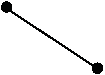
\includegraphics{images/CellConnectionsLine}} &
  \raisebox{-0.5\height}{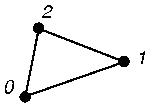
\includegraphics{images/CellConnectionsTriangle}} \\
  \dax{CellTagVertex} \index{vertex} &
  \dax{CellTagLine} \index{line} &
  \dax{CellTagTriangle} \index{triangle} \\[2ex]
  \raisebox{-0.5\height}{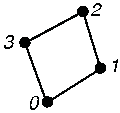
\includegraphics{images/CellConnectionsQuadrilateral}} &
  \raisebox{-0.5\height}{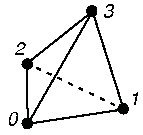
\includegraphics{images/CellConnectionsTetrahedron}} &
  \raisebox{-0.5\height}{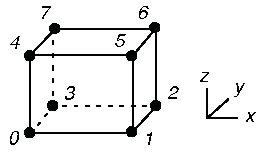
\includegraphics{images/CellConnectionsVoxel}} \\
  \dax{CellTagQuadrilateral} \index{quadrilateral} &
  \dax{CellTagTetrahedron} \index{tetrahedron} &
  \dax{CellTagVoxel} \index{voxel} \\[2ex]
  \raisebox{-0.5\height}{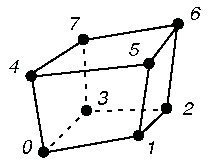
\includegraphics{images/CellConnectionsHexahedron}} &
  \raisebox{-0.5\height}{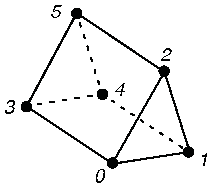
\includegraphics{images/CellConnectionsWedge}} \\
  \dax{CellTagHexahedron} \index{hexahedron} &
  \dax{CellTagWedge} \index{wedge} &
\end{longtable}

\subsubsection{Traits}
\label{sec:CellTraits}

The Dax toolkit has a \dax{CellTraits} templated class that provides
general information about each of the cell
types. \textidentifier{CellTraits} can be used in either the control or
execution environment, but are more commonly used in the execution
environment.

Like other traits classes, \textidentifier{CellTraits} contains static
information that can be used to specialize templates or overload functions
based on general traits. A \textidentifier{CellTraits} class contains the
following items for all known cell tags.

\begin{description}
\item[\textidentifier{NUM\_VERTICES}] \index{NUM\_VERTICES} A static
  constant number set to the number of vertices in the cell.
\item[\textidentifier{TOPOLOGICAL\_DIMENSIONS}]
  \index{TOPOLOGICAL\_DIMENSIONS} A static constant number set to the
  topological dimensions of the cell type. It is 3 for polyhedra, 2 for
  polygons, 1 for lines, and 0 for points.
\item[\textcode{TopologicalDimensionsTag}] \index{TopologicalDimensionsTag}
  Always \textcode{typedef}ed to
  \dax{CellTopologicalDimensionsTag}\textcode{<}\textidentifier{TOPOLOGICAL\_DIMENSIONS}\textcode{>}.
  This tag provides a convenient way to overload a function based on
  topological dimensions (which is often more efficient than conditionals).
\item[\textcode{GridTag}] \index{GridTag} A \textcode{typedef} to a tag
  specifying the type of grid that holds this type of cell. Can be set to
  \dax{GridTagUniform} or \dax{GridTagUnstructured}. These correspond to
  the control environment structures described in
  Section~\ref{sec:GridStructures}.
\item[\textcode{CanonicalCellTag}] \index{CanonicalCellTag} A
  \textcode{typedef} to a tag for a cell type that can be held in an
  unstructured grid that has an equivalent topology as this cell. For
  example,
  \dax{CellTraits}\textcode{<}\dax{CellTagVoxel}\textcode{>::CanonicalCellTag}
  is \textcode{typedef}ed to \dax{CellTagHexahedron}. This trait is useful
  for specializing templates and functions that operate on all cell types
  with equivalent topology. For example, it can be used to create a
  function that operates on cells from an unstructured grid of hexahedra or
  a uniform grid.
\end{description}

\subsubsection{Vertex and Field Information}

\index{vertex|(}
\index{field|(}

When a worklet scheduled on cells is operating on a point field (generally
identified with a \sigtagmod{Field}{Point} tag in the \controlsignature as
described in Section~\ref{sec:ControlSignature}), then the Dax scheduler
pulls all the relevant field values and passes them to the worklet in a
\daxexec{CellField} object. \textidentifier{CellField} is templated first
on the field data type and second on the cell tag. The
\textidentifier{CellField} class has a
\textidentifier{NUM\_VERTICES}\index{NUM\_VERTICES} constant set to the
number of field values in the cell. The \textidentifier{CellField} also has
its bracket operator overloaded to access each field
value. \textidentifier{CellField} also has the methods
\textcode{GetAsTuple} and \textcode{SetFromTuple} to convert to and from a
\dax{Tuple} structure.

It is also possible to get the point indices for each vertex of the
cell. This is done by using the \sigtag{Vertices} tag in the
\executionsignature as described in
Section~\ref{sec:ExecutionSignature}. In this case, the point indices are
placed in a \daxexec{CellVertices} object. A \textidentifier{CellVertices}
object behaves the same as a \textidentifier{CellField} with the field
value type set as \dax{Id}.

The following artificial example uses \daxexec{CellField} and
\daxexec{CellVertices} to make a worklet that finds for each cell the
incident point that has the maximum field value.

\begin{daxexample}{Using \textidentifier{CellField} and \textidentifier{CellVertices}.}
#include <dax/exec/CellField.h>
#include <dax/exec/CellVertices.h>
#include <dax/exec/WorkletMapCell.h>

class FindMaxPointIds : public dax::exec::WorkletMapCell
{
public:
  typedef void ControlSignature(Topology, Field(Point), Field(Out));
  typedef _3 ExecutionSignature(Vertices(_1), _2);

  template<typename CellType, typename FieldType>
  DAX_EXEC_EXPORT
  dax::Id operator()(const dax::exec::CellVertices<CellType> &vertices,
                     const dax::exec::CellField<FieldType,CellType> &fieldValues) const
  {
    int maxVertexIndex = 0;
    FieldType maxFieldValue = fieldValues[0];
    for (int vertexIndex = 1; vertexIndex < fieldValues.NUM_VERTICES; vertexIndex++)
      {
      FieldType fieldValue = fieldValues[vertexIndex];
      if (!(fieldValue < maxFieldValue))
        {
        maxVertexIndex = vertexIndex;
        maxFieldValue = fieldValue;
        }
      }
    return vertices[maxVertexIndex];
  }
};
\end{daxexample}

\index{field|)}
\index{vertex|)}

\subsubsection{Operations}
\label{sec:CellOperations}

The Dax execution environment API comes with several functions and classes
that perform operations on cells. These facilities are templated on cell
tags and operate on \textidentifier{CellField} containers.

\paragraph{Parametric Coordinates}
\label{sec:ParametricCoordinates}

\index{parametric coordinates|(}
\index{world coordinates|(}
\index{cell!parametric coordinates|(}

Each cell type supports a one-to-one mapping between a set of parametric
coordinates in the unit cube (or some subset of it) and the points in 3D
space that are the locus contained in the cell. Parametric coordinates are
useful because certain features of the cell such as vertex location and
center, are at a consistent location in parametric space irrespective of
the location and distortion of the cell in world space. Also, many field
operations are much easier with parametric coordinates.

The \daxheader{dax/exec}{ParametricCoordinates.h} header file contains the
following functions for working with parametric coordinates.

\begin{description}
\item[\daxcont{ParametricCoordinatesToWorldCoordinates}] Given a
  \textidentifier{CellField} of point coordinates and a \dax{Vector3}
  containing parametric coordinates, returns the world coordinates.
\item[\daxcont{WorldCoordinatesToParametricCoordinates}] Given a
  \textidentifier{CellField} of point coordinates and a \dax{Vector3}
  containing world coordinates, returns the parametric coordinates. This
  function can be slow for cell types with nonlinear interpolation (which
  is anything that is not a simplex).
\end{description}

The \daxheader{dax/exec}{ParametricCoordinates.h} header additionally
provides a templated class named \daxexec{ParametricCoordinates}. The
single template argument is a cell tag. This class holds static methods
that return parametric coordinates for special locations. The
\textidentifier{ParametricCoordinates} class contains the following static
functions.

\begin{description}
\item[\textcode{Center}] Returns a \dax{Vector3} containing the parametric
  coordinates for the center of a cell.
\item[\textcode{Vertex}] Returns a \daxexec{CellField} of \dax{Vector3}s
  containing the parametric coordinates for each vertex of a cell.
\end{description}

\index{cell!parametric coordinates|)}
\index{world coordinates|)}
\index{parametric coordinates|)}

\paragraph{Interpolations}

\index{cell!interpolation|(}
\index{interpolation|(}

The shape of every cell is defined by the connections of some finite set of
vertices. Field values defined on those vertices can be interpolated to any
point within the cell to estimate a continuous field.

The \daxheader{dax/exec}{Interpolate.h} header contains the function
\daxexec{CellInterpolate} that takes a \daxexec{CellField} of field values
and a \dax{Vector3} containing parametric coordinates. It returns the
interpolated value of the field. The \daxworklet{PointDataToCellData}
worklet provides a simple example of interpolating fields.

\begin{daxexample}{Interpolating a field to the center of a cell.}
class PointDataToCellData : public dax::exec::WorkletMapCell
{
public:
  typedef void ControlSignature(Topology,Field(Point), Field(Out));
  typedef _3 ExecutionSignature(_2);

  template<class CellTag>
  DAX_EXEC_EXPORT
  dax::Scalar operator()(const dax::exec::CellField<dax::Scalar,CellTag> &pointField) const
  {
    dax::Vector3 center =  dax::exec::ParametricCoordinates<CellTag>::Center();
    return dax::exec::CellInterpolate(pointField,center,CellTag());
  }
};
\end{daxexample}

\index{interpolation|)}
\index{cell!interpolation|)}

\paragraph{Derivatives}

\index{cell!derivative|(}
\index{derivative|(}
\index{gradient|(}

Since interpolations provide a continuous field function over a cell, it is
reasonable to consider the derivative of this function. The
\daxheader{dax/exec/Derivative.h} header file provides the overloaded
function \daxexec{CellDerivative} that computes the partial derivative of a
field with respect to each axis in 3D space (also known as the
\keyterm{gradient}). \textidentifier{CellDerivative} takes 4 arguments: a
\dax{Vector3} containing parametric coordinates of where the gradient
should be found, a \daxexec{CellField} of \dax{Vector3} containing the
point coordinates at each vertex, a \daxexec{CellField} containing the
field values at each vertex, and the tag of the cell type.

The \daxworklet{CellGradient} worklet provides a simple example of finding
field derivatives.

\begin{daxexample}{Finding derivatives of a field at the center of a cell.}
class CellGradient : public dax::exec::WorkletMapCell
{
public:
  typedef void ControlSignature(Topology, Field(Point), Field(Point), Field(Out));
  typedef _4 ExecutionSignature(_2,_3);

  template<class CellTag>
  DAX_EXEC_EXPORT
  dax::Vector3 operator()(const dax::exec::CellField<dax::Vector3,CellTag> &coords,
                          const dax::exec::CellField<dax::Scalar,CellTag> &pointField) const
  {
    dax::Vector3 parametricCellCenter = dax::exec::ParametricCoordinates<CellTag>::Center();
    return dax::exec::CellDerivative(parametricCellCenter, coords, pointField, CellTag());
  }
};
\end{daxexample}

\index{gradient|)}
\index{derivative|)}
\index{cell!derivative|)}

\index{cell|)}

\index{execution~environment|)}


\section{OpenGL Interoperability}
\label{sec:OpenGLInteroperability}

\index{interop|(}
\index{OpenGL|(}

Although it is designed to run on GPUs, the Dax toolkit is not a rendering
library. However, as a toolkit for visualization, it is often desirable to
directly render the results from computations using a rendering library
like OpenGL. In such a circumstance, it is desirable to transfer data in
Dax arrays directly into OpenGL buffers rather than pull back to the CPU
and push again to the in a different context.

To facilitate this direct transfer, the Dax toolkit comes with an OpenGL
interoperability feature. To transfer an array used in the Dax toolkit to
an OpenGL context, use the \daxopengl{TransferToOpenGL} function. The
function takes two arguments. The first argument is a \daxcont{ArrayHandle}
to transfer. The second argument is a reference to a \textcode{GLuint}. If
this argument contains a valid handle to an OpenGL buffer, then that buffer
will point to the array being transferred. Otherwise, a new buffer handle
will be generated and returned in this second argument. The function
returns a \textcode{GLenum} containing the identifier for the OpenGL type
in the OpenGL buffer. An overloaded version version of
\textidentifier{TransferToOpenGL} takes a third argument that specifies the
OpenGL type to use in a \textcode{GLenum}.

\begin{daxexample}{Using OpenGL Interoperability}
DAX_CONT_EXPORT
void BindPointCoordinates(dax::cont::ArrayHandle<dax::Vector3> pointArray)
{
  GLuint oglPointBuffer;
  glGenBuffers(1, &oglPointBuffer);

  dax::opengl::TransferToOpenGL(pointArray, oglPointBuffer);

  glEnableClientState(GL_VERTEX_ARRAY);
  glBindBuffer(GL_ARRAY_BUFFER, oglPointBuffer);
  glVertexPointer(3, GL_FLOAT, 0, NULL);
}
\end{daxexample}

Although the Dax toolkit supports CUDA computations, it also supports
several other types of architectures. Thus, the process for
interoperability changes depending on the device adapter being used. The
Dax interoperability takes this into account and will provide a custom
overload of \textidentifier{TransferToOpenGL} depending on the abilities of
the device adapter. Thus, code that uses the Dax toolkit with OpenGL does
not need to provide conditionals to manage the different types of devices.

\index{OpenGL|)}
\index{interop|)}


\section{Coding Conventions}
\label{sec:CodingConventions}

Several developers contribute to the Dax toolkit and we welcome others who
are interested to also contribute to the project. To ensure readability and
consistency in the code, we have adopted the following coding
conventions. Many of these conventions are adapted from the coding
conventions of the VTK project. This is because many of the developers are
familiar with VTK coding and because we expect the Dax toolkit to have
continual interaction with VTK.

\begin{itemize}
\item All code contributed to Dax must be compatible with Dax's BSD
  license.
\item Copyright notices should appear at the top of all source,
  configuration, and text files. The statement should have the following
  form:
\small\begin{verbatim}
//==========================================================================
//
//  Copyright (c) Kitware, Inc.
//  All rights reserved.
//  See LICENSE.txt for details.
//
//  This software is distributed WITHOUT ANY WARRANTY; without even
//  the implied warranty of MERCHANTABILITY or FITNESS FOR A PARTICULAR
//  PURPOSE.  See the above copyright notice for more information.
//
//  Copyright 2013 Sandia Corporation.
//  Under the terms of Contract DE-AC04-94AL85000 with Sandia Corporation,
//  the U.S. Government retains certain rights in this software.
//
//==========================================================================
\end{verbatim}
  The \textfilename{CopyrightStatement} checks all files for a similar
  statement. The test will print out a suggested text that can be copied
  and pasted to any file that has a missing copyright statement (with
  appropriate replacement of comment prefix). Exceptions to this copyright
  statement (for example, third-party files with different but compatible
  statements) can be added to \textfilename{LICENSE.txt}.
\item All include files should use include guards. starting right after the
  copyright statement. The naming convention of the include guard macro is
  that it should start with two underscores and be followed with the
  path name, starting from the top-level source code directory, with non
  alphanumeric characters, such as \textcode{/} and \textcode{.} replaced
  with underscores. The \textcode{\#endif} part of the guard at the bottom
  of the file should include the guard name in a comment. For example, the
  \daxheader{dax/cont}{ArrayHandle.h} header contains the guard
  \begin{verbatim}
#ifndef __dax_cont_ArrayHandle_h
#define __dax_cont_ArrayHandle_h
\end{verbatim}
  at the top and
  \begin{verbatim}
#endif //__dax_cont_ArrayHandle_h
\end{verbatim}
  at the bottom.
\item The Dax toolkit has several nested namespaces. The declaration of
  each namespace should be on its own line, and the code inside the
  namespace bracket should not be indented. The closing brace at the bottom
  of the namespace should be documented with a comment identifying the
  namespace. Namespaces can be grouped as desired. The following is a valid
  use of namespaces.
  \begin{verbatim}
namespace dax {
namespace cont {

namespace detail {

class InternalClass;

} // namespace detail

class ExposedClass;

}
} // namespace dax::cont
\end{verbatim}
\item Multiple inheritance is not allowed in Dax classes.
\item Any functional public class should be in its own header file with the
  same name as the class. The file should be in a directory that
  corresponds to the namespace the class is in. There are several
  exceptions to this rule.
  \begin{itemize}
  \item Templated classes and template specialization often require the
    implementation of the class to be broken into pieces. Sometimes a
    specialization is placed in a header with a different name.
  \item Many Dax toolkit features are not encapsulated in
    classes. Functions may be collected by purpose or co-located with
    associated class.
  \item Although tags are technically classes, they do not behave as an
    enumeration for the compiler. Multiple tags that make up this
    enumeration are collected together.
  \item Some classes, such as \dax{Tuple} are meant to behave as basic
    types. These are sometimes collected together as if they were related
    \textcode{typedef}s. The \daxheader{dax}{Types.h} header is a good
    example of this.
  \end{itemize}
\item The indentation style can be characterized as the ``indented brace''
  (a modified whitesmith) style. Indentations are two spaces, and the curly
  brace (scope delimiter) is placed on the following line and indented
  along with the code (i.e. the curly brace lines up with the code).
\item Conditional clauses (including loop conditionals such as
  \textcode{for} and \textcode{while}) must be in braces below the
  conditional. That is, instead of
  \begin{verbatim}
if (test) { clause; }
\end{verbatim}
  use
  \begin{verbatim}
if (test)
  {
  clause;
  }
\end{verbatim}
  The rational for this requirement is to make it obvious whether the
  clause is executed when stepping through the code with the debugger. The
  one exception to this rule is when the clause contains a control-flow
  statement with obvious side effects such as \textcode{return} or
  \textcode{break}. However, even if the clause contains a single statement
  and is on the same line, the clause should be surrounded by braces.
\item Use two space indentation.
\item Tabs are not allowed. Only use spaces for indentation. No one can
  agree on what the size of a tab stop is, so it is better to not use them
  at all.
\item There should be no trailing whitespace in any line.
\item Use only alphanumeric characters in names. Use capitalization to
  demarcate words within a name (camel case). The exception is preprocessor
  macros and constant numbers that are, by convention, represented in all
  caps and a single underscore to demarcate words.
\item Namespace names are in all lowercase. They should be a single word
  that designates its meaning.
\item All class, method, member variable, and functions should start with a
  capital letter. Local variables should start in lower case and then use
  camel case. Exceptions can be made when such naming would conflict with
  previously established conventions in other library. (For example,
  \textcode{make\_Vector2} corresponds to \textcode{make\_pair} in the
  standard template library.)
\item Always spell out words in names; do not use abbreviations except in
  cases where the shortened form is widely understood and a name in its own
  right (e.g. OpenMP).
\item Always use descriptive names in all identifiers, including local
  variable names. Particularly avoid meaningless names of a few characters
  (e.g. \textcode{x}, \textcode{foo}, or \textcode{tmp}) or numbered names
  with no meaning to the number or order (e.g. \textcode{value1},
  \textcode{value2},\ldots). Also avoid the meaningless for loop variable
  names \textcode{i}, \textcode{j}, \textcode{k}, etc. Instead, use a name
  that identifies what type of index is being referenced such as
  \textcode{pointIndex}, \textcode{vertexIndex}, \textcode{componentIndex},
  etc.
\item Classes are documented with Doxygen-style comments before classes,
  methods, and functions.
\item Exposed classes should not have public instance variables outside of
  exceptional situations. Access is given by convention through methods
  with names starting with \textcode{Set} and \textcode{Get} or through
  overloaded operators.
\item References to classes and functions should be fully qualified with
  the namespace. This makes it easier to establish classes and functions
  from different packages and to find source and documentation for the
  referenced class. As an exception, if one class references an internal or
  detail class clearly associated with it, the reference can be shortened
  to \textcode{internal::} or \textcode{detail::}.
\item use \textcode{this->} inside of methods when accessing class methods
  and instance variables to distinguish between local variables and
  instance variables.
\item Include statements should generally be in alphabetical order. They
  can be grouped by package and type.
\item Namespaces should not be brought into global scope or the scope of
  any Dax package namespace with the ``using'' keyword. It should also be
  avoided in class, method, and function scopes (fully qualified namespace
  references are preferred).
\item All code must be valid by the C++03 and C++11 specifications. It must
  also compile on older compilers that support C++98. Code that uses
  language features not available in C++98 must have a second
  implementation that works around the limitations of C++98. The
  \cmakevar{DAX\_FORCE\_ANSI} turns on a compiler check for ANSI
  compatibility in gcc and clang compilers.
\item Limit all lines to 80 characters whenever possible.
\item New code must include regression tests that will run on the
  dashboards. Generally a new class will have an associated ``UnitTest''
  that will test the operation of the test directly. There may be other
  tests necessary that exercise the operation with different components or
  on different architectures.
\item All code must compile and run without error or warning messages on
  the nightly dashboards, which should include Windows, Mac, and Linux.
\item Use \dax{Scalar} in lieu of \textcode{float} or \textcode{double} to
  represent data for computation and use \dax{Id} in lieu of \textcode{int}
  or \textcode{long} for data structure indices. This future-proofs code
  against changes in precision of the architecture. The indices of
  \dax{Tuple} are an exception. Using \textcode{int} to reference
  \dax{Tuple} (and other related classes like \daxexec{CellField} and
  \daxmath{Matrix}) indices are acceptable as it is unreasonable to make
  these vectors longer than the precision of \textcode{int}.
\item All functions and methods defined within the Dax toolkit should be
  declared with \daxcontexport, \daxexecexport, or \daxexeccontexport.
\end{itemize}

We should note that although these conventions impose a strict statute on
Dax coding, these rules (other than those involving licensing and
copyright) are not meant to be dogmatic. Examples can be found in the
existing code that break these conventions, particularly when the
conventions stand in the way of readability (which is the point in having
them in the first place). For example, it is often the case that it is more
readable for a complicated \textcode{typedef} to stretch a few characters
past 80 even if it pushes past the end of a display.

